\documentclass[pdftex,dvipsnames]{dissertation}

% --- Encoding stuff ----------------------------------------------------------
\usepackage[utf8]{inputenc}
\usepackage[T1]{fontenc}

% --- English stuff -----------------------------------------------------------
\usepackage[english]{babel}

\usepackage{xspace}
\usepackage{csquotes}

% --- Debug stuff -------------------------------------------------------------
\usepackage{morewrites} % workaround for "no room for new \write" error

% --- Font stuff --------------------------------------------------------------
\usepackage{stackengine} % for overlapping text

% --- Blind text --------------------------------------------------------------
\usepackage{blindtext} % provide \blindtext, \Blindtext
\usepackage{lipsum}

\usepackage{xargs}   % Use more than one optional parameter in a new commands
\usepackage{xcolor}  % Coloured text etc.

% --- TODO notes --------------------------------------------------------------
\usepackage[colorinlistoftodos,prependcaption,textsize=small,shadow]{todonotes}
% my alias
\newcommand{\itodo}[1]{\todo[inline]{#1}\PackageWarning{TODO ::}{#1}}
\newcommand{\miss}[1]{\todo[inline,backgroundcolor=white,bordercolor=black]{#1}\PackageWarning{TODO ::}{#1}}
\newcommandx{\unsure}[2][1=]{\todo[linecolor=red,backgroundcolor=red!25,bordercolor=red,#1]{#2}\PackageWarning{TODO ::}{#2!}}
\newcommandx{\change}[2][1=]{\todo[linecolor=blue,backgroundcolor=blue!25,bordercolor=blue,#1]{#2}\PackageWarning{TODO ::}{#2!}}
\newcommandx{\info}[2][1=]{\todo[linecolor=OliveGreen,backgroundcolor=OliveGreen!25,bordercolor=OliveGreen,#1]{#2}\PackageWarning{TODO ::}{#2!}}
\newcommandx{\plus}[2][1=]{\todo[linecolor=Plum,backgroundcolor=Plum!25,bordercolor=Plum,#1]{#2}\PackageWarning{TODO ::}{#2!}}

% --- Symbols, Units and Icons ------------------------------------------------
\usepackage{fontawesome} % fontawesomeicons

% --- Math --------------------------------------------------------------------
\usepackage{kmath} % cool delimiters
\usepackage{dsfont} % double stroke
\usepackage[mathscr]{euscript}
\usepackage{xfrac} % provide \sfrac, cool fractions
\usepackage{siunitx}    % provide \ang and SI units

% --- Theorem environment------------------------------------------------------
\usepackage{amsthm}
\usepackage{thmtools}
\usepackage{thm-restate}
\declaretheorem[%
    name=Rationale,
    refname={Rationale,Rationales},
    Refname={Rationale,Rationales}
]{rationale}
\declaretheorem[%
    name={Security Claim},
    numbered={unless unique},
]{secclaim}

% --- Packages from Frederich -------------------------------------------------
\usepackage{longtable}
\usepackage{pdflscape}
\usepackage{enumitem}

%%% OTHER INCLUDES
\newrobustcmd*{\fullfullcite}{%
    \AtNextCite{%
        \AtEachCitekey{%
            \defcounter{maxnames}{99}%
            \DeclareNameAlias{labelname}{given-family}%
        }%
    }%
    \fullcite
}

%% IMAGE AS SYMBOL

% % set the Bison QED symbol
% \renewcommand{\qed}{%
% \leavevmode\unskip\penalty9999 \hbox{}\nobreak\hfill%
% \quad\hbox{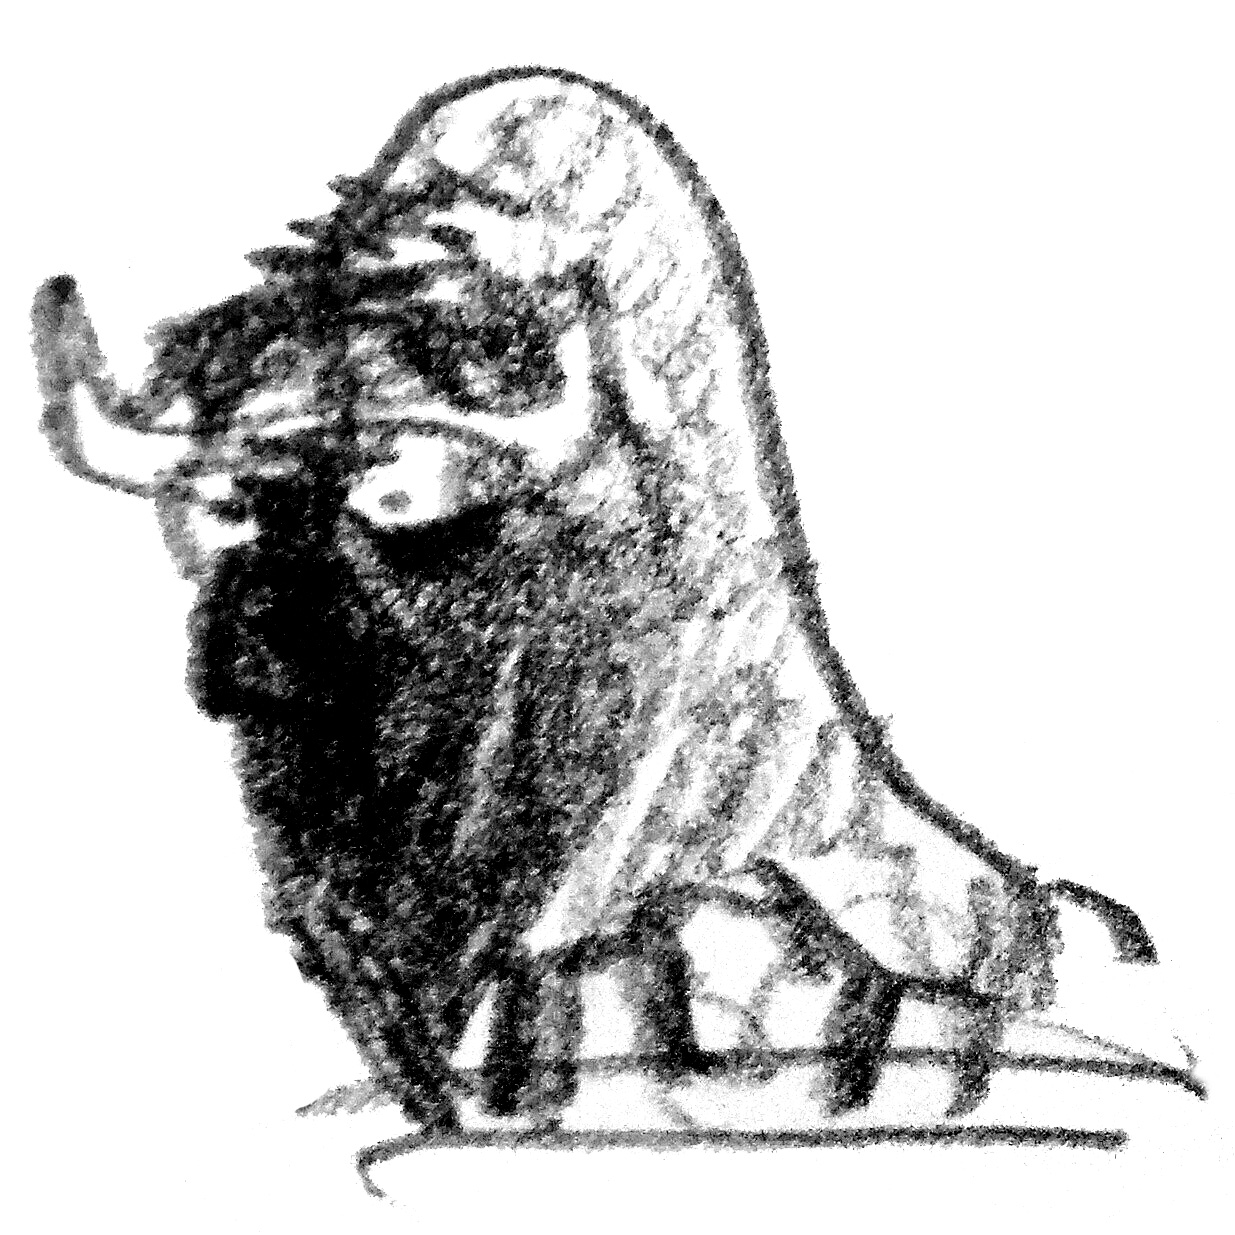
\includegraphics[height=1em]{bison/bison-qed.jpg}}}

\newcommand{\cpother}[1]{{\color{BlueGreen} #1}}
\newcommand{\cpmine}[1]{{\color{GreenYellow} #1}}

% --- my abbreviation ---------------------------------------------------------
\newcommand{\imgsrc}[1]{Image courtesy of #1}
\newcommand{\cfr}[1]{\Cf/ #1}

% --- math models -------------------------------------------------------------
\newcommand{\echoModelFreq}{\ensuremath{
    H_{ij}(f_k) = \sum_{\idxEch=0}^{\numEchs}
        \frac{\absCoeff_{ij}^r}{4 \pi \speedOfSound \tau_{ij}^r}
        \cste^{- \csti 2 \pi k \Fs \tau_{ij}^r / F}}}

\newcommand{\sumEcho}{\ensuremath{\sum_{\idxEch=0}^{\numEchs}}}
\newcommand{\echoModelTimeSimple}[1]{\ensuremath{\sumEcho \alpha_{#1}^{(r)} \delta(t - \tau_{#1}^{(r)})}}
\newcommand{\alltaus}[1]{\ensuremath{\{\tau_{#1}^{(r)}\}_{#1,r}}}
\newcommand{\allalphas}[1]{\ensuremath{\{\alpha_{#1}^{(r)}\}_{#1,r}}}

\newcommand{\icon}[1]{\raisebox{-.1\height}{\includegraphics[height=3ex]{#1}}}
\newcommand{\chaosIcon}{\icon{figures/blaster/chaos.png}}
% --- correct bad hyphenation
\hyphenation{op-tical net-works semi-conduc-tor}

% --- Algos and Methods names:
\newcommand{\mirage}{\textsc{Mirage}}
\newcommand{\separake}{\textsc{Separake}}
\newcommand{\brioche}{\textsc{Brioche}}
\newcommand{\blaster}{\textsc{Blaster}}
\newcommand{\blasterr}{\textsc{Blaster2}}
\newcommand{\lantern}{\textsc{Lantern}}
\newcommand{\dechorate}{d'\textsc{Echorate}}

%----------------
\usepackage{pgffor}
% for math stuff
\foreach \x in {a,...,z}{
  % mathbf
  \expandafter\xdef\csname bf\x \endcsname{\noexpand\ensuremath{\noexpand\mathbf{\x}}}
  % Bold symbol
  \expandafter\xdef\csname bs\x \endcsname{\noexpand\ensuremath{\noexpand\boldsymbol{\x}}}
  % Typewriter
  \expandafter\xdef\csname tt\x \endcsname{\noexpand\ensuremath{\noexpand\mathtt{\x}}}
}

\foreach \x in {A,...,Z}{
%   % Bold symbol -- bold
  \expandafter\xdef\csname bs\x \endcsname{\noexpand\ensuremath{\noexpand\boldsymbol{\x}}}
%   % mathbf -- bold
  \expandafter\xdef\csname bf\x \endcsname{\noexpand\ensuremath{\noexpand\mathbf{\x}}}
%   % mathbb -- blackboard-bold for uppercase letters and lowercase ( for sets )
  \expandafter\xdef\csname bb\x \endcsname{\noexpand\ensuremath{\noexpand\mathbb{\x}}}
%   % mathds -- ???
  \expandafter\xdef\csname ds\x \endcsname{\noexpand\ensuremath{\noexpand\mathds{\x}}}
%   % mathfrak -- gothic
  \expandafter\xdef\csname fk\x \endcsname{\noexpand\ensuremath{\noexpand\mathfrak{\x}}}
%   % mathfrak -- curly
  \expandafter\xdef\csname scr\x \endcsname{\noexpand\ensuremath{\noexpand\mathscr{\x}}}
%   % mathcal -- calligraphy
  \expandafter\xdef\csname cal\x \endcsname{\noexpand\ensuremath{\noexpand\mathcal{\x}}}
}

% --- Math Notation
% math
\newcommand{\Ii}{\ensuremath{\imath}}
% \newcommand{\cstj}{\ensuremath{\jmath}}
\newcommand{\R}{\ensuremath{\bbR}}
\newcommand{\N}{\ensuremath{\bbN}}
\newcommand{\Z}{\ensuremath{\bbZ}}
% indexing
\newcommand{\idxSrc}{\ensuremath{j}}
\newcommand{\idxMic}{\ensuremath{i}}
\newcommand{\idxEch}{\ensuremath{r}}
\newcommand{\numSrcs}{\ensuremath{J}}
\newcommand{\numMics}{\ensuremath{I}}
\newcommand{\numEchs}{\ensuremath{R}}
% geometry
\newcommand{\positionMicrophone}{\ensuremath{\underline{\bfx}}}
\newcommand{\positionSource}{\ensuremath{\underline{\bfs}}}
\newcommand{\positionSurface}{\ensuremath{\underline{\bfp}}}
\newcommand{\pos}{\ensuremath{\bfr}}
\newcommand{\coordinatePermutation}{\ensuremath{\bfR}}
\newcommand{\distMicSrc}{\ensuremath{r}}
\newcommand{\distMicMic}{\ensuremath{d}}
% signal model
\newcommand{\src}{\ensuremath{s}}
\newcommand{\mic}{\ensuremath{x}}
\newcommand{\mics}{\ensuremath{\bsx}}
\newcommand{\img}{\ensuremath{c}}
\newcommand{\imgs}{\ensuremath{\bsc}}
\newcommand{\spat}{\ensuremath{\boldsymbol{\Xi}}}
\newcommand{\master}{\ensuremath{\boldsymbol{\Upsilon}}}
\newcommand{\contRecordedSignal}{\ensuremath{x}}
\newcommand{\contMicrophoneSignal}{\contRecordedSignal}
\newcommand{\contSource}{\ensuremath{s}}
\newcommand{\contFilter}{\ensuremath{h}}
\newcommand{\contFilterHat}{\widehat{\contFilter}}
\newcommand{\contRIR}{\contFilter}
\newcommand{\contNoise}{\ensuremath{n}}
\newcommand{\disRecordedSignal}{\bfx}
\newcommand{\disFilter}{\bfh}
\newcommand{\disFilterHat}{\widehat{\disFilter}}
\newcommand{\RecordedSignalDFT}{\bfX}

% (room) acoustics
\newcommand{\speedOfSound}{\ensuremath{c}}
\newcommand{\cair}{\ensuremath{\speedOfSound_\text{air}}}
\newcommand{\temperature}{\ensuremath{T}}
\newcommand{\rhumidity}{\ensuremath{H}}
\newcommand{\forceVec}{\ensuremath{\bsF}}
\newcommand{\velocity}{\ensuremath{\bsv}}
\newcommand{\pressure}{\ensuremath{p}}
\newcommand{\Pressure}{\ensuremath{P}}
\newcommand{\flux}{\ensuremath{\bsq}}
\newcommand{\density}{\ensuremath{\rho}}
\newcommand{\densityEq}{\density_0}
\newcommand{\mass}{\ensuremath{m}}
\newcommand{\volumeUnit}{\ensuremath{\nu}}
\newcommand{\surface}{\ensuremath{S}}
\newcommand{\volume}{\ensuremath{\calV}}
\newcommand{\impedence}{\ensuremath{Z}}
\newcommand{\impedenceAir}{\ensuremath{\impedence_\text{air}}}
\newcommand{\absCoeff}{\ensuremath{\alpha}}
\newcommand{\reflCoeff}{\ensuremath{\beta}}
\newcommand{\boundariesConditions}{\ensuremath{\calB}}
\newcommand{\wavelength}{\ensuremath{\lambda}}
\newcommand{\ntuple}{\ensuremath{\bsm}}

\newcommand{\depSpaceTime}{\ensuremath{\kparen{\positionMicrophone, t}}}
\newcommand{\pressureSpaceTime}{\ensuremath{\pressure\depSpaceTime}}

% signal processing
\newcommand{\error}{\ensuremath{{\varepsilon}}}
\newcommand{\filterLength}{\ensuremath{{L}}}
\newcommand{\Ts}{\ensuremath{T_s}}
\newcommand{\Fs}{\ensuremath{F_s}}
\newcommand{\zeroVect}{\ensuremath{\mathbf{0}}}
\newcommand{\rir}{\ensuremath{h}}
\newcommand{\rirFreq}{\ensuremath{H}}
\newcommand{\rirs}{\ensuremath{\bsh}}
\newcommand{\rtf}{\ensuremath{\tilde{\rir}}}
\newcommand{\rtfs}{\ensuremath{\tilde{\rirs}}}
\newcommand{\ild}{\ensuremath{\mathtt{ILD}}}
\newcommand{\ipd}{\ensuremath{\mathtt{IPD}}}

% math vars and constant
\newcommand{\spike}[1]{\delta_{#1}}
\newcommand{\opObs}{\calA}
\newcommand{\thr}{\tau_\text{max}}
\newcommand{\algoBraire}{BLASTER}
\newcommand{\algoBsn}{BSN}
\newcommand{\algoCrocco}{IL1C}

% variable
\newcommand{\RT}{\ensuremath{\mathtt{RT}_{60}}}
\newcommand{\DRR}{\ensuremath{\mathtt{DRR}}}
\newcommand{\DER}{\ensuremath{\mathtt{DER}}}
\newcommand{\SNR}{\ensuremath{\mathtt{SNR}}}
\newcommand{\dsetValid}{$\mathbf{\mathcal{D}}^{\:\text{(valid)}}$}
\newcommand{\dsetSNR}{$\mathbf{\mathcal{D}}^{\:\SNR}$}
\newcommand{\dsetRT}{$\mathbf{\mathcal{D}}^{\:\RT}$}

% --- Other (constant)
\newcommand{\const}{\ensuremath{\text{\textit{const.}}}}

\newcommand{\idealLowPassFilter}{\phi}
\newcommand{\disRadonMeasure}{\calM(\Theta)}
\newcommand{\posDisRadonMeasure}{\calM_+(\Theta)}

% \newcommand{\m1}{\mathbf{m}_1}
% \newcommand{\m2}{\mathbf{m}_2}
% \newcommand{\s}{{\mathbf s}}
% \newcommand{\params}{\mathbf{\theta}}

% --- Quantities names

% --- Mathematical Delimiters

% % syntactically named delimiters
% \newdelimcommand{ceil}{\lceil}{\rceil}
% \newdelimcommand{floor}{\lfloor}{\rfloor}
% \newdelimcommand{angles}{\langle}{\rangle}
% \newdelimcommand{parens}{\lparen}{\rparen}
% \newdelimcommand{bracket}{[}{]}
% \newdelimcommand{braces}{\lbrace}{\rbrace}
% \newdelimcommand{verts}{\lvert}{\rvert}
% \newdelimcommand{Verts}{\lVert}{\rVert}

% % semantically named delimiters
\newcommand{\set}[1]{\kbrace{#1}}
% \newcommand{\abs}{\verts}
% \newcommand{\size}{\verts}
\newcommand{\abs}[1]{\kvbar{#1}}
\newcommand{\norm}[1]{\kvvbar{#1}}
\newcommand{\normTV}[1]{\ensuremath{\norm{#1}_{\mathtt{TV}}}}
% \newcommand{\tuple}{\angles}
% \newcommand{\iprod}{\angles}

% % Automagic `such that' for set comprehension. Inside an automagic
% % delimiter command, the vertical bar will resize appropriately
% % Example:
% %   \set{ x \in W \given x > 0 }
\newcommand{\given}{\;\mdelim\vert\;}


% --- Math operators
\DeclareMathOperator*{\fourierTrans}{\scrF}
\DeclareMathOperator*{\discreteFT}{\bfF}
\DeclareMathOperator*{\divergence}{\nabla\cdot}
\DeclareMathOperator*{\dirac}{\delta}
\newcommand{\average}{\operatornamewithlimits{average}}

% --- Mathematical operators and function
\newcommand{\conv}{\ast}
\newcommand{\diracOf}[1]{\dirac\kparen{#1}}
\DeclareMathOperator*{\phase}{\angle}
\newcommand{\phaseOf}[1]{\phase{#1}}
\newcommand{\magnitudeOf}[1]{\abs{#1}}
\newcommand{\powerOf}[1]{\abs{#1}^2}


% other definition
\newcommand{\myeq}{\mathrel{\overset{\makebox[0pt]{\mbox{\normalfont\tiny\sffamily def}}}{=}}}
\newcommand{\mathspace}{\hspace{1em}}

%%% MACROS
\newcommand{\gc}[1]{{\textcolor{green}{#1}}}
% \newcommand{\gc}[1]{{\textcolor{black}{#1}}}

\newcommand{\gccor}[2]{{\textcolor{red}{[#1 $\rightarrow$ #2]}}}
% \newcommand{\gccor}[2]{{\textcolor{black}{#2}}}

\newcommand{\gccmt}[1]{{\textcolor{blue}{[SE: #1]}}}
%\newcommand{\gccmt}[1]{}

\newcommand{\gcrm}[1]{{\textcolor{magenta}{[#1]}}}
% \newcommand{\gcrm}[1]{{\textcolor{black}{}}}

% --- Table of Contents -------------------------------------------------------
%%% TOC STYLE : check in the dissertation class
% check dissertation class
% %% MINITOC per CHAPTER
\usepackage{minitoc} % must be inserted after any modification of TOC

% --- Graphics ----------------------------------------------------------------
\usepackage{pgfplots}
\pgfplotsset{compat=1.8}
\usepgfplotslibrary{fillbetween} %for fill under curve
\usepackage{tikz}
\usetikzlibrary{fadings}
\usetikzlibrary{patterns}
\usetikzlibrary{shadows.blur}
\usetikzlibrary{shapes}
\usepackage[abs]{overpic}
\graphicspath{{./figures/}{./icons/}{./logos/}}
\DeclareGraphicsExtensions{.pdf,.png,.jpg}

% \pgfplotsset{%
%     table/search path={./figures/plots/},
% }

% --- Bibliopgraphy -----------------------------------------------------------
\bibliography{contents/back_matter/references.bib}


% --- Include only ------------------------------------------------------------
% \includeonly{   % Of course this list allows many more file
% %  intro,       % should also work with files in different paths
%     chapter1_acoustics,
%     chapter2_processing,
%     chapter3_evaluation,
% %  chapter3
% }

%%%%%%%%%%%%%%%%%%%%%%%%%%%%%%%%%%%%%%%%%%%%%%%%%%%%%%%%%%%%%%%%%%%%%%%%%%%%%%%
%%%%%%%%%%%%%%%%%%%%%%%%%%%%%%%%%%DOCUMENT%%%%%%%%%%%%%%%%%%%%%%%%%%%%%%%%%%%%%
%%%%%%%%%%%%%%%%%%%%%%%%%%%%%%%%%%%%%%%%%%%%%%%%%%%%%%%%%%%%%%%%%%%%%%%%%%%%%%%

\title{Hunting Acoustic Echoes for Auditory Scene Analysis}
\author{Diego DI CARLO}
\date{\today}

\begin{document}
\frontmatter{}

% front matter / titelei
% recto: halftitlepage / schmutztitelseite, vortitel
\thispagestyle{empty}
{
    \begin{fullwidth}
        \centering
        \hphantom{.}
        \vfill
        {\Huge
            Hunting Echoes\\
            for\\
            Auditory Scene Analysis
        }
        \vfill
        \vfill
    \end{fullwidth}
}

\clearpage{}

% verso: frontispiece / frontiszipzseite, vakatseite
% dedication
\cleardoublepage{}

% recto: titlepage / titelblatt, innentitel
\thispagestyle{empty}
{
    \calccentering{\unitlength}
    \begin{adjustwidth*}{\unitlength}{-\unitlength}
        \raggedleft{}
        {\Huge\color{Burgundy}%
        Hunting Echoes\\
        for Auditory Scene Analysis}\\[\baselineskip]
        {\LARGE%
        Dissertation Thesis}\\[0.2\textheight]
        {\huge%
        Diego \textsc{Di Carlo}}\\[\baselineskip]
        {\LARGE%
        \today}
        \vfill
        \vfill
        {\large%
        Submitted in partial fulfillment of the requirements\\
        for the degree of Doktor der Naturwissenschaften\\[\baselineskip]% (Dr.\ rer.\ nat.)\\[\baselineskip]

        to the\\[\baselineskip]

        Faculty of Mathematics\\
        at Ruhr-Universität Bochum\\[2\baselineskip]
        %Vorgelegt zur Erlangung des\\
        %Doktorgrades der Naturwissenschaften\\
        %an der Fakultät der Mathematik\\
        %der Ruhr-Universität Bochum\\[2\baselineskip]

        \begin{minipage}{0.5\textwidth}
        \begin{tabular}{lr}
            1st\hspace{4pt} Reviewer & Prof.\ Dr. Gregor Leander\\
            2nd Reviewer & Prof.\ Dr.\; Alexander May
        \end{tabular}
        \end{minipage}
        \hspace*{36pt}
        %}\hspace*{-8pt}

        %\vspace{2\baselineskip}
        %Datum der Disputation: 13.\ Dezember 2019
        \vfill
        }
        \vspace*{\baselineskip}
    \end{adjustwidth*}
}

\clearpage{}

% verso: colophon / impressum
\thispagestyle{empty}
\hphantom{.}
\vfill

\section*{Imprint}

\textit{Hunting Echoes for Audtory Scene Analysis}\\
Copyright \textcopyright{} 2020 by \theauthor{}.\\
All rights reserved. Printed in France.\\
Published by the Ruhr-Universität Bochum, Bochum, Germany.

\section*{Colophon}

This thesis was typeset using \LaTeX{} and the \texttt{memoir} documentclass.
It is based on Aaron Turon's thesis \emph{Understanding and expressing scalable concurrency}\footnote{\url{https://people.mpi-sws.org/~turon/turon-thesis.pdf}}, itself a mixture of \texttt{classicthesis}\footnote{\url{https://bitbucket.org/amiede/classicthesis/}} by Andr\'e Miede and \texttt{tufte-latex}\footnote{\url{https://github.com/Tufte-LaTeX/tufte-latex}}, based on Edward Tufte's \emph{Beautiful Evidence}.\\[0.5\baselineskip]
%
The bibliography was processed by Biblatex.
All graphics and plots are made with PGF/Ti\emph{k}Z.\\[0.5\baselineskip]
%
The body text is set 10/14pt (long primer) on a 26pc measure.
The margin text is set 8/9pt (brevier) on a 12pc measure.
Matthew Carter's \textrm{Charter} acts as both the text and display typeface.
Monospaced text uses Jim Lyles's \texttt{Bitstream Vera Mono} (\enquote{Bera Mono}).

\clearpage{}

% recto: dedication or epigraph
\thispagestyle{empty}
\vphantom{.}
\vfill
{%
    \flushright{}
    \emph{Pleasure to me is wonder—the unexplored, the unexpected, \\
    the thing that is hidden and the changeless thing\\
    that lurks behind superficial mutability.}\\
    \hfill--- Howard Phillips \textsc{Lovercraft}
}
\vfill
\vfill

% verso: blank
\clearpage{}


\chapter*{Abstract}\addcontentsline{toc}{chapter}{Abstract}

Audio\marginpar{
    \footnotesize
    \textbf{Keywords:}
    \\Acoustic echoes, acoustic echo retrieval, room impulse response estimation;
    audio scene analysis, room acoustics;
    audio source separation, room geometry estimation, spatial filtering, sound source localization;
    deep learning, continuous dictionary.
} scene analysis aims at retrieving useful information from microphone recordings.
Examples of these problems are sound source separation and sound source localization, where we are interested in estimating the content and location of multiple sources of sound in an environnement.
As humans, we perform these tasks without effort. However, for computers and robots, they are still open challenges.
One of the main limitations is that most available technologies solve audio scene analysis problems either ignoring how sound propagates in the environment or estimating it fully.

\mynewline
The central theme of this theses is acoustic echoes: the sound propagation elements bridging semantic and spatial information on sound sources.
Indeed, as repetitions of a source signal, their semantic contributions can be aggregated to enhance this signal.
Moreover, since they originate from an interaction with the environment, their paths can be backtracked and used to estimate the audio scene's geometry.
Based on these observations, recent echo-aware audio signal processing methods have been proposed.
However, two main questions arise: how to estimate acoustic echoes, and how to use their knowledge?

\mynewline
This thesis work aims at improving the current state-of-the-art for indoor audio signal processing along these two axes.
It also provides new methodologies and data to process acoustic echoes and surpass current approaches' limits.
To this end, in the first part, we present two approaches:
a novel approach based on the  continuous dictionary framework which does not rely on parameter tuning or peak picking techniques;
a deep learning model estimating the time differences of arrival of the first prominent echoes using physically-motivated regularizers.
Furthermore, we present a novel, fully annotated dataset specifically designed for acoustic echo retrieval and echo-aware applications, paving the way for future echo-aware research.

\mynewline
The second part of this thesis focuses on extending existing methods in audio scene analysis to their echo-aware forms.
The Multichannel NMF framework for audio source separation, the SRP-PHAT localization method, and the MVDR beamformer for speech enhancement are extended to in their echo-aware versions.
These applications show how a simple echo model can lead to a boost in performance.

\newthought{This thesis} highlights the difficulty of exploiting acoustic echoes to improve indoor audio processing.
As a first attempt to lay unified analytical and methodological foundations for these problems, it is hoped to serve as a starting point for promising new research in this field.
% Finally, we want to underline the difficulty related to the tasks of estimating and exploiting acoustic echoes to improve indoor audio processing.
% Therefore, this thesis consists only of a first attempting work that lays analytical foundations on how to model such problems, and it can serve as a starting point for new exciting directions.
\blankpage{}
\chapter*{Résumé en français}\addcontentsline{toc}{chapter}{Résumé en français}

% This summary presents in French an overview of the work addressed in this thesis.

% The audio scene analysis topic covers many different tasks that aim to retrieve useful information from microphone recordings.
% Examples of these problems are sound source separation and sound source localization, where we are interested in estimating a speaker's content and position.
% As humans, we perform these tasks without effort: imagine someone calling us from the other side of the room. Your typical reaction would probably turn your attention towards or even go to him/her.
% However, for computers and robots, using audio signal processing techniques, are still open challenges.

% Sounds convey semantic information (what your friends said), temporal and spatial (when he said it, where he said it).
% We can model these contributions using signals describing the sound content and room impulse response, accounting for its propagation in the space. Some audio processing methods focus on the former, ignoring or roughly describing the latter due to the challenging task of estimating it.
% Room Impulse responses embed all the elements of sound propagation, such as echoes, diffuse reflection, and reverberation.

% The central theme of this theses are acoustic echoes. These elements of sound propagation create a bridge between semantic and spatial information of sound sources. As they are repetitions and copies of the source sound, we can weigh more the target sound by integrating their contribution than other noise sources.
% As these reflections are originated by the interaction of the source sound with the environment, thanks to their arrival time, we can retrace back their paths and, thus, reconstruct the geometry of the audio scene's geometry.
% Based on these observations, audio signal processing methods started to account for these sound propagation elements to solve the audio scene analysis problem.
% Two are the main questions that arise:
% how we estimated acoustic echoes, and how we use their knowledge?

% This thesis work aims at improving the current state-of-the-art for indoor audio signal processing along these two axes.
% In particular, it provides new methodologies and data to process acoustic echoes and surpass current approaches' limits.
% Second, it extends previous classical methods for audio scene analysis in their echo-aware form.
% These two claims are elaborated in the two main parts of the thesis, which follow after an introductory one, as summarized below.

% First, we provide some preliminary definitions of the role of audio signal processing and list some fundamental problems which will be considered throughout the thesis, namely, acoustic echo retrieval, audio source separation, sound source localization, room geometry estimation.

% The~\cref{ch:acoustics} will build a first important bridge: from acoustics to audio signal processing. It first defines sound, how it propagates in the environment, and how this origins echoes.

% In~\cref{ch:processing},  we move from physic to digital signal processing where the echoes are modeled as elements of filters, called Room Impulse Responses (RIRs), operating on the source signal.
% Because processing in the native time domain is complicated, we present the Fourier representation, which facilitates both the exposure of the methods and the implementation of the algorithms.
% This chapter closes the first introductory part.

% In this second part of the thesis, we are interested in estimating early acoustic echoes from microphone recordings. Based on the models and the definition described in the first part, this part includes first a general overview of echo retrieval methods followed by the presentation of two works published at international conferences and a dataset that is about to be released.

% First, in chapter~\cref{ch:estimation}, we provide the reader with knowledge of the state-of-the-art about Acoustic Echo Retrieval, namely, on how to estimate acoustic echoes properties. After presenting the problem and the literature is review according to typical taxonomy used in signal processing. In order to provide a complete look at Acoustic Echo Retrieval, some datasets and evaluation metrics recurring in the literature and used in the following chapter are presented.

% In this second part of the thesis, we are interested in estimating early acoustic echoes from microphone recordings.
% Based on the models and the definition described in the first part, this part includes first a general overview of echo retrieval methods followed by the presentation of two works published at international conferences and a dataset that is about to be released.

% First, in chapter~\cref{ch:estimation}, we provide the reader with knowledge of the state-of-the-art about Acoustic Echo Retrieval, namely, on how to estimate acoustic echoes properties. After presenting the problem and the literature is review according to typical taxonomy used in signal processing. In order to provide a complete look at Acoustic Echo Retrieval, some datasets and evaluation metrics recurring in the literature and used in the following chapter are presented.

% The following three chapters presented three works we conducted on Acoustic Echo Estimation.

% \cref{ch:blaster} presents a novel approach for estimating echoes from a stereophonic recording of an unknown sound source such as speech.  In contrast with existing methods, it is built on the recent continuous dictionary framework and does not rely on parameter tuning or peak picking techniques.
% The method's accuracy and robustness are assessed on challenging simulated setups with varying noise and reverberation levels and are compared to two state-of-the-art methods. Experimental evaluation on synthetic data shows that comparable or slightly worse recovery rates are observed for recovering seven echoes or more. Instead, better results are obtained for a fewer number of echoes, and the off-grid nature of the approach yields generally smaller estimation errors.
% Nevertheless, this is promising since the practical advantage of knowing the timing few echoes per channel will be demonstrated in the last part of the thesis.

% In~\cref{ch:lantern}, we deploy deep learning techniques to estimate acoustic echoes properties. To the best of our knowledge, this is one of the first examples in these directions. The proposed method shares some common grounds with deep learning techniques already applied in sound source localization. We will present three different architecture which addresses the acoustic echo estimation problem with increasing order of complexity: estimating the time of arrival of the direct path and the first prominent echos; perform this estimation in a more robust way; and, finally, extend it to an increasing number of echoes.

% Finally, to conclude this second part, in~\cref{ch:dechorate}, we describe a dataset we collected, specifically designed for acoustic echo estimation. This dataset features measured multichannel room impulse response (RIRs), including annotations of early echoes and 3D positions of microphones and real and image sources under different wall configurations in a cuboid room. These data provide a new tool for benchmarking recent methods in \textit{echo-aware} audio signal processing and software utilities to easily access, manipulate, and visualize the data.

% The third and last part of the thesis concern the audio processing applications where the knowledge of early echoes may improve the performance over standard methods.
% For the occasion, we assume that echoes properties are available a priori and build our prior knowledge.
% The structure of this part follows the format of the previous one.

% An introductory chapter gathers the standard definitions and introduces the current state-of-the-art approaches for indoor audio processing under the same umbrella.
% We consider three fundamental problems: audio source separation, sound source localization, spatial filtering, and room geometry estimation.
% These problems are presented in turn with the related literature review, highlighting the current challenges.
% These particular problems will be the protagonist of the following three chapters, presented in their echo-aware form.

% In~\cref{ch:separake}, echoes are used for boosting the performance of classical Audio Source Separation methods and results from a collaboration with other colleagues, published in an international conference.
% In particular, we propose a physical interpretation of the echoes, namely, image microphones, which allow understanding better how the algorithms benefit from their knowledge.
% Our investigation considers two variants of the multichannel nonnegative matrix factorization source separation framework: one that uses only magnitudes of the transfer functions and uses the phases.
% The results show that the proposed approach beats its vanilla variant by using only a few echoes and echoes enable separation where it was considered unaffordable.

% \cref{ch:mirage} addresses the problem of audio source localization in the context of strong acoustic echoes. Using the model of image microphones presented in the previous chapter, we show that these interfering contributions can be used to change the classic way source localization performed.
% In particular, we show that in a simple scenario involving two microphones close to a reflective surface and one source, the proposed approach is able to estimate both azimuthal and elevation angles, impossible task assuming an ideal propagation, as classical approaches do.
% These results were merged into a publication, published in an international conference.
% Furthermore, the investigation is then extended to microphone arrays featuring multiple sensors and to real-world data, provided by a collaboration with the research team of Honda.

% The ~\cref{ch:dechorateapp} presents two echo-aware applications that can benefit from the dataset \dEchorate, presented in~\cref{ch:dechorate}. We exemplify the utilization of these data considering two possible audio scene analysis problems: echo-aware spatial filtering and room geometry estimation.
% In order to validate the data and show their potential, well-known state-of-the-art algorithms are used. Therefore, for each of the applications, the considered methods are contextualized and summarized.
% Numerical results confirm the value of this dataset for the audio signal processing community. The dataset and these methods will be released publicly so that external contributors will be invited to use them for developing more robust audio processing methods.

% The last chapter (\cref{ch:conclusing}) recapitulates the main results presented in this manuscript and the perspectives related to this work.
% Among them, we show how few acoustic echoes can be estimated from the only observation of microphone recordings featuring reverberant speech using either model derived from the physics of the sound propagation and deep learning models trained on acoustic simulators.
% Moreover, we demonstrate the strengths of including the knowledge of acoustic echoes in audio processing methods.
% For the aspect related to the evaluation of echo-aware methods in a real-world scenario, we advocate that freely-available benchmarking datasets are currently missing in the literature. Therefore, in the spirit of open research, we build a new dataset which will soon be released. These data are accompanied by accurate annotation and algorithmic tools for echo-aware research covering much application for audio scene analysis.

% Finally, we want to underline the difficulty related to the task of estimating and exploiting acoustic echoes to improve indoor audio processing. This thesis, therefore, consists only in a first attempting work that lays analytical foundations on how to model such problems.
% Like all the first investigations, a lot can be improved, and we hope it can serve as a starting point for new interesting, and challenging researches.
\blankpage{}

\chapter*{Acknowledgements}\addcontentsline{toc}{chapter}{Acknowledgements}

Block ciphers form, without doubt, the backbone of today's encrypted communication and are thus justifiably the workhorses of cryptography.
While efficiency of modern designs improved ever since the development of the DES and AES, the case with the corresponding security arguments differs.
The thesis at hand aims at two main points, both in the direction of improving security analysis of block ciphers.

Part~I studies a new notion for the better understanding of a special type of cryptanalysis and proposes a new block cipher instance.
This instance comes with a tight bound on any differential, to the best of our knowledge the first such block cipher.

Part~II turns to automated methods in design and analysis of block ciphers.
Our main contribution here is an algorithm to propagate subspaces through encryption rounds, together with two applications: an algorithmic security argument against a new type of cryptanalysis and an idea towards the automation of key recovery attacks.

\cleardoublepage{}

%*******************************************************
% Table of Contents
%*******************************************************
\doparttoc[n]
\tableofcontents*\addcontentsline{toc}{chapter}{Contents}
\clearpage{}

% \chapter{Glossary}*\addcontentsline{toc}{chapter}{Glossary}%
\marginpar{
    \footnotesize
    \textbf{Glossary:}
    \begin{itemize}
        \item A list of terms in a particular domain of knowledge with their definitions.
        \item From Latin \textit{glossarium} ``collection of glosses'', diminutive of \textit{glossa} ``obsolete or foreign word''.
    \end{itemize}
}
% === GLOSSARY ===
\begin{acronym}[UMLX]
    \acro{AB}{Almost Bent}
    \acro{ACT}{Autocorrelation Table}
    \acro{AES}{Advanced Encryption Standart}
    \acro{ANF}{Algebraic Normal Form}
    \acro{APN}{Almost Perfect Nonlinear}
    \acro{ASIC}{Application Specific Integrated Circuit}
    \acro{BCT}{Boomerang Connectivity Table}
    \acro{BCT}{Boomerang Connectivity Table}
    \acro{CBC}{Cipher Block Chaining}
    \acro{CCA}{Chosen Ciphertext Attack}
    \acro{CFB}{Cipher Feedback}
    \acro{CPA}{Chosen Plaintext Attack}
    \acro{CTR}{Counter}
    \acro{DDT}{Difference Distribution Table}
    \acro{DES}{Data Encryption Standart}
    \acro{DLCT}{Differential-Linear Connectivity Table}
    \acro{DP}{Differential Probability}
    \acro{ECB}{Electronic Codebook}
    \acro{EDP}{Expected Differential Probability}
    \acro{ELP}{Expected Linear Potential}
    \acro{FPGA}{Field Programmable Gate Array}
    \acro{IoT}{Internet-of-Things}
    \acro{KPA}{Known Plaintext Attack}
    \acro{LAT}{Linear Approximation Table}
    \acro{LFSR}{Linear Feedback Shift Register}
    \acro{LP}{Linear Potential}
    \acro{LUT}{Look Up Table}
    \acro{LWC}{Lightweight Crypto}
    \acro{MDS}{Maximum Distance Separable}
    \acro{MEDP}{Maximum Expected Differential Probability}
    \acro{MELP}{Maximum Expected Linear Potential}
    \acro{MILP}{Mixed Integer Linear Program}
    \acro{OFB}{Output Feedback}
    \acro{OTP}{One Time Pad}
    \acro{PRP}{Pseudo\-random Permutation}
    \acro{SLP}{Straight-Line Program}
    \acro{SPN}{Substitution Permutation Network}
    \acro{WSN}{Whitened Swap-Or-Not}

    % --- ch:intro
    \acro{CASA}{Computational Auditory Scene Analysis}
    % --- ch:acoustics
    \acro{SOTA}{State of the Art}
    \acro{GA}{Geometrical (room) acoustics}
    \acro{FEM}{Finite Element Method}
    \acro{BEM}{Boundary Element Method}
    \acro{FDTD}{Finite-Difference-Time-Domain}
    \acro{DWM}{Digital Waveguide Mesh}
    \acro{ISM}{Image Source Method}
    \acro{TOA}{Time of Arrival}
    \acro{RIR}{Room Impulse Response}
    \acro{ReIR}{Relative Impulse Response}
    \acro{FIR}{Finite Impulse Resposne}
    \acro{ATF}{Acoustic Transfer Function}
    \acro{AIR}{Acoustic Impulse Response}
    \acro{TF}{Time-Frequency}
    % --- ch:processing
    \acro{SE}{Speech Enhancement}
    \acro{SSS}{Sound Source Separation}
    \acro{SSL}{Sound Source Localization}
    \acro{RooGE}{Room Geometry Estimation}
    \acro{AER}{Acoustic Echo Retrieval}
    \acro{FT}{Fourier Transform}
    \acro{DFT}{Discrete Fourier Transform}
    \acro{DTFT}{Discrete-Time Fourier Transform}
    \acro{STFT}{Short Time Fourier Transform}
    \acro{FFT}{Fast Fourier Transform}
    \acro{RTF}{Relative Transfer Function}
    \acro{ILD}{Interchannel Level Difference}
    \acro{IPD}{Interchannel Phase Difference}
    \acro{ITD}{Interchannel Time Difference}
    \acro{TDOA}{Time Difference of Arrival}
    \acro{AWGN}{Additive White Gaussian Noise}
    % --- ch:aer
    \acro{AER}{Acoustic Echo Retrieval}
    \acro{MLS}{Minimum Length Sequence}
    \acro{ESS}{Exponential Sine Sweep}
    \acro{ML}{Maximum Likelihood}
    \acro{MUSIC}{Multiple Signal Classification}
    \acro{ESPRIT}{Estimation of Signal Parameters via Rational Invariance Techniques}
    \acro{SSL}{Sound Source Localization}
    \acro{RooGE}{Room Geometry Estimation}
    \acro{JADE}{Joint Angle and Delay Estimation}
    \acro{DOA}{Direction of Arrival}

\end{acronym}
\cleardoublepage{}
\clearpage{}

% \listofalgorithms\addcontentsline{toc}{chapter}{List of Algorithms}
% \vspace{\baselineskip}
% \clearpage{}
%*******************************************************
% List of Figures
%*******************************************************
\listoffigures*\addcontentsline{toc}{chapter}{List of Figures}
\vspace{\baselineskip}
\clearpage{}

\listoftables*\addcontentsline{toc}{chapter}{List of Tables}
\clearpage{}

\chapter*{Notations}\addcontentsline{toc}{chapter}{Notations}\label{ch:notation}

\section*{Linear Algebra}
\begin{table}[H]
    \begin{tabular}{ll}
        $x, X$     & scalars      \\
        $\bsx, \bfx$  & vectors      \\
        $x_i$   & $i$-th entry of $\bfx$ \\
        $\zeroVect_I$ & $I\times1$ vector of zeros\\
        $\ktranspose{\bfx}$   & transpose of the vector $\bfx$ \\
        $\khermitian{\bfx}$   & conjugate-transpose (Hermitian) of the vector $\bfx$ \\
        $\kRe[x]$ & real part scalar (vector) $x$ ($\bfx$) \\
        $\kIm[x]$ & imaginary part scalar (vector) $x$ ($\bfx$) \\
        $\csti$  & imaginary unit \\
        $\bbN$    & set of natural numbers \\
        $\bbR$    & set of real numbers \\
        $\bbR_{+}$  & set of real positive numbers \\
        $\bbC$      & set of complex numbers \\
    \end{tabular}
\end{table}

\section*{Common indexing}
\begin{table}[H]
    \begin{tabular}{ll}
        $i$     & microphone or channel index in $\{0, \ldots, I-1\}$      \\
        $j$     & source index in $\{0, \ldots, J-1\}$      \\
        $r$     & reflection (echo) index in $\{0, \ldots, R-1\}$      \\
        $t$     & continuous time index\\
        $n$     & discrete sample index in $\{0, \ldots, N-1\}$ \\
        $f$     & continuous frequency index in $\set{0, \ldots, T-1}$\\
        $k$     & discrete frequency index in $\{0, \ldots, F-1\}$ \\
        $l$     & discrete time-frame index in $\{0, \ldots, L-1\}$\\
        $\tau$  & continuous tap index
    \end{tabular}
\end{table}

\section*{Geometry}
\begin{table}[H]
    \begin{tabular}{ll}
        $\positionMicrophone_i$ & 3D position of the microphone $i$ recording $x_i(t)$\\
        $\positionSource_j$ & 3D position of the source $j$ emitting $s_j(t)$\\
        $\distMicMic_{ii'}$           & distance between microphone $i$ and $i'$ \\
        $\distMicSrc_{ij}$     & distance between microphone $i$ and source $j$ \\
        $r_{j}$    & distance of source $j$ \wrt/ to a reference frame \\
        $\theta_{j}$    & azimuth of source $j$ \wrt/ to a reference frame\\
        $\varphi_{j}$    & elevation of source $j$ \wrt/ to a reference frame \\
        $\vartheta_{j}$    & angle of arrival of source $j$ \wrt/ to a reference frame \\
    \end{tabular}
\end{table}

\section*{Signals}
\begin{table}[H]
    \begin{tabular}{ll}
        $\tildex(t)$    & continuous time domain signal\\
        $x[n]$          & discrete time domain signal\\
        $x_N[n]$          & discrete and finite time domain signal\\
        $\tildeX(f)$    & continuous frequency domain\\
        $X[k]$          & discrete frequency domain\\
        $X[k,l]$        & discrete time domain\\
                        &                     \\
        $x_i$     & input signal recorded at microphone $i$\\
        $\bsx$    & $I \times 1$ multichannel input signal, i.e. $\bfx = [x_0, \ldots, x_{I-1}]$ \\
        $\bsH$    & matrix of multichannel signal or filters, typically the mixing matrix ($I \times J$)\\
        $s_j$     & (target) point source signal $j$ \\
        $q_j$     & (interfering) point source signal $j$ \\
        $c_{ij}$  & spatial image source $j$ as recorded at microphone $i$\\
        $a_{ij}$  & acoustic impule response from source $j$ to microphone $i$ \\
        $h_{ij}$  & generic filter from source $j$ to microphone $i$ \\
        $n_{i}$   & (white \textbf{or} distortion) noise signal at microphone $i$\\
        $u_{i}$   & generic interfering \textbf{and} distortion noise signal at microphone $i$ \\
        $\varepsilon_{i}$   & generic noise signal due to mis- or under-modeling $i$ \\
    \end{tabular}
\end{table}

\section*{Acoustic}
\begin{table}[H]
    \begin{tabular}{ll}
        $\alpha_{r}$    & attenuation coefficient at reflection $r$\\
        $\beta_{r}$     & reflection coefficient at reflection $r$\\
        $\tau_{r}$      & time instant of the reflection $r$\\
        $\cair$         & speed of sound in air\\
        $\temperature$  & temperature\\
        $\rhumidity$    & relative humidity\\
        $\pressure$     & sound pressure\\
        $\rir_{ij}$     & Room Impulse Response from source $j$ to microphone $i$ \\
    \end{tabular}
\end{table}

\section*{Mathematical Operations}
\begin{table}[H]
    \begin{tabular}{ll}
        $\convCont$          & continuous time convolution\\
        $\convDis$       & discrete linear convolution\\
        $\convCir$       & discrete circular convolution\\
    \end{tabular}
\end{table}

% \section*{Examples}

% Simple time domain echo model:
% \begin{equation*}
%     a_i(t) = \echoModelTimeSimple{}
% \end{equation*}
\cleardoublepage{}

\setcounter{mtc}{9}

% === MAIN BODY ===
\mainmatter{}

%% PROLOGE
% \begin{fullwidth}
%     \part{Prologue}
% \end{fullwidth}
% \parttoc[n]
% \cleardoublepage{}

\chapter{Overture}\label{chap:intro}

\openepigraph{Only echoes answer me.}{Anton Chekhov, Swan Song}
\openepigraph{\textsc{Écho.} Citer ceux du Panthéon et du pont de Neuilly. }{Gustave Flaubert, Dictionnaire des idées reçues}

\section{Preamble}
Animals and humans have a remarkable ability to listen to the acoustic response of their environment.
Also known as \emph{echolocation} or \emph{bio-sonar}, it is used consciously and unconsciously to retrieve
information about the environment and objects using sound waves.
Two (of the most) striking examples are bats and whales which use it as navigation and foraging mechanisms.


\marginpar{%
    \begin{itemize}
        \item[\faYoutube] \href{https://www.youtube.com/watch?v=lLUcOFwZvyY&t=22s}{Testing The World's Longest Echo}
        \item[\faYoutube] \href{https://www.youtube.com/watch?v=px3oVGXr4mo}{What Does Sound Look Like? | SKUNK BEAR}
        \item[\faYoutube] arte
    \end{itemize}

}

Definitions of: In this thesis, an \textit{auditory scene} consists in \textit{sound sources}, \textit{microphones} deployed in a room.


\section{The Problem}\label{sec:intro:problem}
\subsection{Audio Signal Processing}
\begin{itemize}
    \item Motivation
    \item Definitions, Function, Characteristics
    \item Current challenges
\end{itemize}
\newthought{Inverse Problem}
Starting with the effects to discover the causes has concerned physicists for centuries.

While in many ways, mixtures are not different to any other audio signal, two research questions stand out prominently: • Can we obtain the sources sj from the mixture x? • Can we find the number of sources J from x? These two questions are addressed in the scientific fields of sound
source separation and source count estimation


Inverse problems appear when we want to see or examine something that we cannot access directly. What we have is an indirect measurement that contains hidden information.

An inverse problem is always a counterpart of a direct problem, as shown in the schematic diagram below. The direct problem is going from object to data, and the inverse problem is about finding the object back from the data.

The assumed few thousand taps. This model was very popular in the early stages of research [48]–[55]. Recently, interest has revived with sparse penalties which account for prior knowledge about the physical properties of AIRs, namely the facts that power concentrates in the direct path and the first early echoes [56]– [60] and that the time envelope decays exponentially [61], but these penalties have not yet been used in a BSS context.

\subsection{Echo-aware Processing}
In the everyday context, when a sound reflection is perceived distinctly is referred to as \textit{echo}.
While phenomenon can be observed clearly in outdoors environment, such in the mountains or within huge buildings,
in closed rooms it is less noticeable. In fact, echoes are usually masked by a general reverberation of the room.

\begin{itemize}
    \item Motivation
    \item Definitions, Function, Characteristics
    \item Current challenges
\end{itemize}

Auralization is the process of rendering audible, by physical or mathematical modelling, the sound field
of a source in a space, in such a way as to simulate the binaural listening experience at a given position in the modelled space

\section{Audio Inverse Problems}\label{sec:processing:inverse}
\cite{kitic2015cosparse}
\openepigraph{Their generality is of such a wide scope that onemayeven argue that solving inverse problems is what signal processing is all about}{Srdan Kiti\'c, \textit{Cosparse regularization of physics-driven inverse problems}}
\openepigraph{everything is an optimization problem}{\citeonly{watson2001nonlinear}}
\marginpar{
    \footnotesize
    One can see the paralelism with the engineering concepts: analysis and sythesis.
}
In~\cref{sec:intro:problem} we have informally defined \textit{inverse problems}, with an emphasis on inverse problems in signal processing.
An inverse problem is a type of a mathematical problem where we start with the observations and we want to estimate model parameters that produced them.
\\Inverse problems pervades all the field of science and engineering:
source localization~\cite{},
image processing~\cite{},
acoustic imaging and tomography~\cite{},
\marginpar{
    \footnotesize
    A historical example are the calculation of the Earth circunference by Eratosthenes in III century b.c.\\
    and the calculations of Adams and Le Verrier which led to the discovery of Neptune from the perturbed trajectory of Uranus.
}

A inverse problems is defined as the counterpart of a \textit{forward}\sidenote{often referred to as \textit{direct}} problem.
Without falling in and deep mathematical formalism and taxonomies which can be found in \citeonly{bal2012introduction},
we will simply consider the following informal definition:
\begin{center}
    \textit{\emph{Forward problem} starts from known input, while \emph{inverse problem} starts from known output~\cite{santamarina2005discrete}.}
\end{center}
Both these problems focus on an operation relating maps objects of interest, called \textit{parameters} or \textit{variables},
to information collected about these objects, called \textit{measurements}, \textit{data} or \textit{observation}.

For instance, in our context, the direct problem may be the estimation of the \RIR/(s) starting from the known room parameters,
and, the related inverse problem would be the estimation of such room properties from the observation of the \RIR/(s).

Formally, a forward problem is defined through a mathematical model, described by a \textit{operation} $\scrM(\cdot)$
mapping \textit{parameters} $x \in \scrX$ to the \textit{observation} (or measurement) $y \in \scrY$:
\begin{equation}\label{eq:processing:model}
    y = \scrM(x)
    .
\end{equation}
Then, the inverse problem defines a method $\kinv{\scrM}$ that ``reverts'' $\scrM$ in order to recover (estimate) $x$ form the observation of $y$.
% The operator $\scrM$ describes our best effort to construct a \textit{model} for the available data $y$.
% The choice of $\scrX$ describes our best effort to characterize the space where we believe the parameters belong.

As discussed in~\cite{bal2012introduction}, \textit{solving} the inverse problem consists in finding point(s) $x \in \scrX$ from (knowledge of) data $y \in \scrY$
such that~\cref{eq:processing:model} or an approximation of~\cref{eq:processing:model} holds.
Under this light, the operator $\scrM$ ant the choice of $\scrX$ describes our best effort to construct a \textit{model} for the data $y$ and
the space where the parameters $x$ belong, respectively.
\marginpar{
    \footnotesize
    one can already see the paralelism the the definition of the mixing process defined in~\cref{sec:intro:problem}
}

\textsc{For instance, in Case of} \textit{linear} inverse problem, and for $\scrY$ and $\scrX$ being vector spaces of dimensions $M$ and $N$ respectively,
then the forward map can be written as a linear system:
\begin{equation}\label{eq:processing:linear_forward}
    \bfy = \bfM \bfx
\end{equation}
where $\bfM$ being a matrix, namely the operator $\scrM$ becomes a matrix multiplication by $M$.
It follows that the inverse map associated to~\cref{eq:processing:linear_forward} is the application of the inverse matrix $\kinv{M}$.
% While solving a direct problem the an operator needs to be found, in solving the inverse one either the operator is known and needs
% to be $reverts$t

Typically, forward problems are considered somehow the ``easier''.
In fact, even in the observation model $\scrM$ is known perfectly, it is not always possible to find its counterpart.
This because of
\begin{itemize}
    \item presence of \textit{noise} in the measurement which are not always additive and statistically independent \wrt/ $x$.
    \item the problem is \textit{well-posed} and \textit{well-conditioned}, namely $\scrM$ needs be injective and stable.
    In other words, some information is recoverable, other is completely lost, other highly sensible to noise
    \sidenote{
        \textbf{injective} ensure the uniqueness of the solution, while \textbf{stability}
        ensure a continuity on the data.
        These are known as the Hadamard's \textit{solvability conditions}.
    }.
\end{itemize}

As we could images, many interesting and fundamental inverse problem are
\textit{ill-posed} or \textit{ill-conditioned} in general, even in the following ``simple'' ones~\cite{kitic2015cosparse}:
The solution to the deconvolution problem, where the direct inversion of the transfer function results in instabilities
at high frequency; and the solution a linear system $\bfy = \bfM \bfx$ where $\bfM$ is invertible
may lead to erroneous results and numerical instabilities.

Therefore, sometimes ones have to settle for restring the set of solution $\scrC \subset \scrX$,
where $\scrM$ is stable and injective\sidenote{This framework was originally proposed by Tikhonov.}.
Promoting solution $x \in \scrC$ is can be achieved through \textit{model priors}, namely prior knowledge about solution, which can
be classified in the following methodologies:
the usage of \textit{geometric constraints} that deterministically define the solutions; the imposition of \textit{penalization}
which ``promotes'' solution of a certain shape (\eg/ \textit{sparse}
\sidenote{\textbf{sparsity} is a fundamental concept of this thesis, better discussed in~\cref{pt:estimation}
} or \textit{smoothness});
and casting the problem in a \textit{bayesian framework} which versatilely incorporate prior and posterior density function describing the data.

\subsection{General Processing Scheme}
Digital signal processing (DSP) is the process of analyzing and modifying a signal to optimize or improve its efficiency or performance. It involves applying various mathematical and computational algorithms to analog and digital signals to produce a signal that's of higher quality than the original signal.
It is traditional in engineering to represent complex systems as a collection of simpler subsystems, with well-defined tasks, interacting with each other.
In signal processing, these subsystems roughly fall into four categories: \textit{representation}, \textit{enhancement}, \textit{estimation}, and \textit{adaptive processing}.
Many problems can be decomposed into blocks that belong to one of these categories.

\begin{description}
    \item[Representation] Objects can be represent (described) in many different way.
    Through different representations, some object \textit{information} becomes more relevant and suitable for certain tasks
    than other.
    \\Representation can be lossy or lossless, and are generally implemented through (non)linear mapping, such as change of basis or feature.
    The most famous representation is the Fourier basis.
    \\Depending on the task the representation may be invertible.
    The process of changing representation is often called: Analysis and Synthesis

    \item[Enhancement] Measurement are affected by noise and interferences which corrupt and hide relevant information, making inverse problems ill-posed and ill-conditioned.
    Therefore, signal enhancement, that is removing noise, is a necessary step.
    \\Enhancement constitute a huge dome of methods: form simple denoising by averaging of repeated measurement to
    spectral subtraction to source separation with neural network.

    \item[Estimation] Often we wish to estimate some key properties of the target signal which may be used as inputs to a different algorithm.

    \item[Adaptive processing] deals with adaptive algorithms and filters controlled by variable parameters.
    A common means to adjust those parameters according to an optimization algorithm which rely on statistical properties of the signal of interest.
    They often implement a kind of online optimization where an objective function is being minimized.
    When new data is observed, its discrepancy with the current estimate is used to produce a new estimate in a way that reduces the objective.
\end{description}

Let us give two example of practical systems that will be recurrent thought out the entire thesis.

\subsection{Selected Audio Inverse Problems}
Here follow some famous problems in the field of audio signal processing with application to speech, music and environmental audio.
Given the mixing process defined in~\cref{sec:processing:model},

% \begin{description}
%     \item[sound source separation and enhancements] as the problem of retrieving a (set of) source signal from a mixture.
%     \item[sound source localization] estimation of source location from the observation of the sound production.
%     This has sense as long as the impulse response convey space properties.
%     \item[microphones calibration] estimation of the microphone placement.
%     \item[\RIR/ estimation] estimation of the filters.
%     Blind Channel Estimation or System Identification.
%     \item[Acoustic Echoes Estimation] estimation of the filters
%     \item[dereverberation] estimation of the filters
%     \item[room geometry estimation] estimation of the room
%     \item[automatich speech recognition]
% \end{description}

\begin{table}[!h]

    \begin{fullwidthfig}
    \centering
    \small

    \begin{tabular}{p{0.33\linewidth}|p{0.66\linewidth}}
        \toprule
        Inverse Problem & \textit{Can we estimate the...} \\
        \hline
        Audio Source Separation  & the signal of the sources $s_{j}$ from the mixture $\boldsymbol{x}$? \\

        Sound Source Localization & the position $\mathbf{s}_{j} \ =\ [ x_{s_{j}} ,\ y_{s_{j}} ,\ z_{s_{j}}]$  of the source $s_{j}$ from the mixture $\boldsymbol{x}$$ $? \\

        Microphone (Array) Calibration & the position of the microphone (array) position $\mathbf{x}$ from the mixture $\boldsymbol{x}$? \\

        \RIR/ Estimation & the filter between the sources $\boldsymbol{s}_{j}$ and the mixture $\boldsymbol{x}$ from $\boldsymbol{x}$? \\

        Room Geometry Estimation & the shape of the room in which the mixture $\boldsymbol{x}$ recoding source $s_{j}$? \\
        \bottomrule
    \end{tabular}

    \end{fullwidthfig}

    \vspace{-\baselineskip}\vspace{-\baselineskip}
    \sideparmargin{outer}
    \sidepar{\vspace{\baselineskip}
        \caption{Selected audio inverse problems}
    }
    \label{tab:processing:problems}


\end{table}

\openepigraph{Everything is connected}{Douglas Adams, \textit{Dirk Gently's Holistic Detective Agency}}
\newthought{Depending on the scenario}, all these problems exhibits strong inter-connections,
namely the solution of one may be (dependent on) the solution of another.
Therefore, exploiting expertise and knowledge,
interconnect and hierarchical approaches may be built\sidenote{Machine Learing allows now for end2end approaches}:
for instance, many spatial filtering techniques used for \SE/ rely on \SSL/ blocks;
and in order to achieves \RooGE/, \AER/ must be done.


\section{My Thesis}
\subsection{Hunting Acoustic Echoes}
\subsection{Echo-aware Auditory Scene Analysis}


\section{Organization and Contributions}
\newthoughtpar{Room Acoustic meets Signal Processing}
\subparagraph{\cref{chap:acoustics}}\blindtext
\subparagraph{\cref{chap:processing}}\blindtext
\subparagraph{\cref{chap:evaluation}}\blindtext

\newthought{Hunting Acoustic Echoes}
\subparagraph{\cref{chap:estimation}}\blindtext
\subparagraph{\cref{chap:lantern}}\blindtext
\subparagraph{\cref{chap:blaster}}\blindtext
\subparagraph{\cref{chap:blasterr}}\blindtext


\newthought{Echo-aware Auditory Scene Analysis}
\subparagraph{\cref{chap:application}}\blindtext
\subparagraph{\cref{chap:separake}}\blindtext
\subparagraph{\cref{chap:mirage}}\blindtext
\subparagraph{\cref{chap:brioche}}\blindtext


Finally, the dissertation concludes with Chapter X, which summarizes
the contributions and raises several additional research questions


\section{This Thesis: Don't Panic!}
The reader will have already noticed that a large margin is left free on the right side of each page of the manuscript.
We will use it to insert comments, historical notes as well as figures and tables to complete the subject.
This graphic charter is inspired by the work of Tufte (2001) and produced using the latex tufte-latex class.
We emphasize that the presence of the clickable GitHub logo in the margin indicates the online availability of the codes.

\newthought{Quick vademecum} for the readers:
\begin{itemize}
    \item Bibliographic references are denoted as \cite{kuttruff2016room}.
    \item Figures, Tables and other floating objects as well as equations are numbered within the chapter number.
    \item Equations are referred as~\cref{eq:acoustics:green_definition}
    \item The main matter of the Thesis’s manuscript starts at page 1, until page 103.
    \item The back matter covers the list of the candidate’s publications and the bibiographic references cited along the text.
    \item Small notes on the margin might be used to easily navigate through the Example of margin note manuscript. They are meant to summarize paragraphs/blocks of text.
    \item The end of the chapter is shown by the following sign between horizontal rules.
\end{itemize}

%% I. Room Acoustic
\begin{fullwidth}
    \part{Room Acoustic meets Signal Processing}
\end{fullwidth}
\parttoc[n]
\chapter{Element of Room Acoustics}\label{chap:acoustics}
\marginpar{%
    \centering
    \footnotesize
    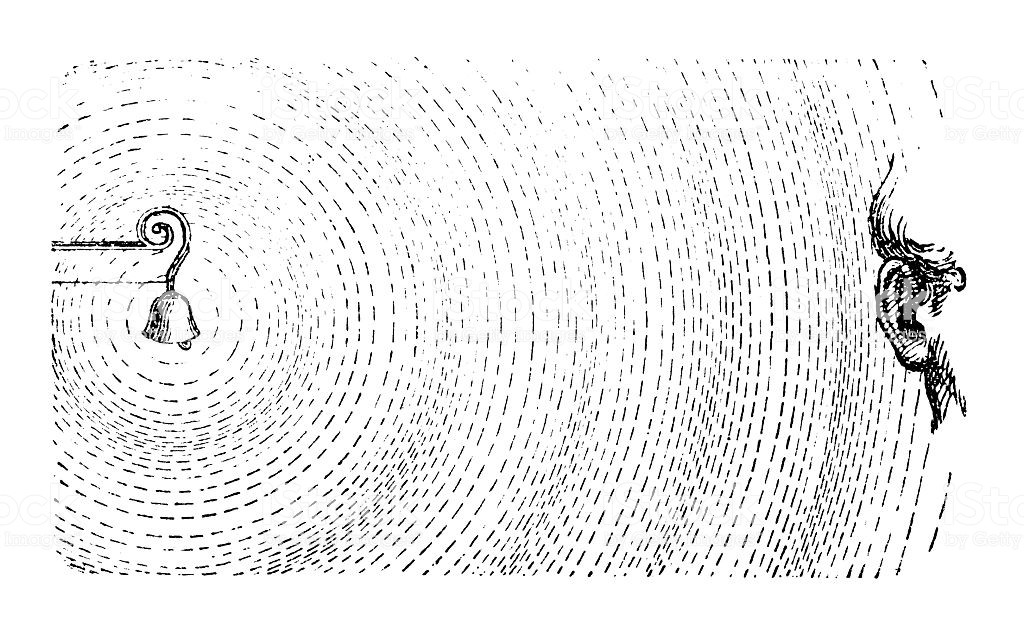
\includegraphics[width=\linewidth]{acoustics/sound_propagation.jpg}
    \label{fig:acoustics:sound}
}
\openepigraph{Sound, a certain movement of air.}{Aristotele, De Anima II.8 420b12}
\vspace{-2.5em}
\newthought{Synopsis}
This chapter will build a first important bridge: from the physics to analog signal processing.
% Acoustics explains how sounds works in environment, while room acoustic explain sound in enclosed spaces, such as living rooms, offices, concert halls and many others.
It first defines sound and how its propagation~\cref{ch:acoustics:sec:wave} connected the concept of impulse response.
Then the interaction with the environment is show~\cref{ch:acoustics:sec:reflection}, teasing out the fundamental concept of this thesis: the echoes.
By assuming some approximation, the \RIRdef/ will be defined.
Finally, a description of the way the human auditory system perceives the sound will be reported.
In particular, the influence of the first early reflection on the sound perception will be elaborated.
One of the most frequently effects produced during sound propagation in a medium is reverberation,
which is caused by physical surfaces that partly absorb and partly reflect sound waves in air. We will first examine in Sec. 4.2 the physical and perceptual background of reverberation. The knowledge gained on these aspects will enable us to study some of the most known reverberation algorithms in Sec. 4.3. Finally we will review in Sec. 4.4 more recent approaches to synthetic reverberation, that are based on feedback delay networks and waveguide meshes.
The rest of the section is reproduce the derivation of this equation, re-arranging the derivation presented in \cite{kuttruff2016room, pierce2019acoustics, marczuk2006modelling, avanzini2019sound}.

\section{Sound Wave Propagation}\label{ch:acoustics:sec:wave}
\marginpar{%
    \small
    Noun: from Middle English sownde, alteration of sowne, borrowed from Anglo-Norman sun, soun, Old French son, from accusative of Latin sonus.
}
According to common dictionaries and encyclopedias,
\begin{center}
    \textit{sound is the sensation perceived by the ear caused by the vibration of air}.
\end{center}
Sound has then two aspects: a physical one, characterized by the vibrating air particles; and a perceptive one, involving the an auditory system.
\marginpar{
    \small
    It is legit to interrogate about where is the sounds.
    % If the sounds we hear have spatial locations, they can be thought to be located either where the material sources are (distal theories), or where the hearers are (proximal theories), or somewhere in between (medial theories). It has also been denied that sounds have any spatial locations, which gives rise to a fourth class of theories, aspatial theories.
    % Proximal theories would claim that sounds are where the hearer is.
    % Medial theories—exemplified by mainstream acoustics—locate sounds in the medium between the resonating object and the hearer.
    % Distal theories consider sounds to be located at the resonating object. Finally, aspatial theories deny spatial relevance to sounds.
}
Focusing on the former phenomenon, when vibrating objects excites air, air molecules starts oscillating,
producing zones with different air densities (compressions-rarefactions)\sidenote{%
Sound needs a medium to travel: it cannot travel through a vacuum.
\\Unfortunately, there is no sound in outer space.
}.
Such vibration of molecules takes place in the direction of the excitement, with the next layer of molecules excited by the first layer.
Pushing layer by layer forward, a \textit{longitudinal wave} is created.
Under a this perspective,
\begin{center}
    \textit{sound is a longitudinal, mechanical wave}.
\end{center}
\marginpar{
    \small
    % In a longitudinal wave the particle displacement is parallel to the direction of wave propagation.
    % In a transverse wave the particle displacement is perpendicular to the direction of wave propagation.
    As opposed to mechanical vibrations in a string or (drum) membrane,
    acoustic vibrations are \textit{longitudinal} rather than \textit{transversal},
    \ie/ the air particles are displaced in the same direction of the wave propagation.
}
A \textit{wave} is a disturbance that propagates though a medium, which could be solid, liquid or gaseous.
\marginpar{%
    \centering
    \footnotesize
    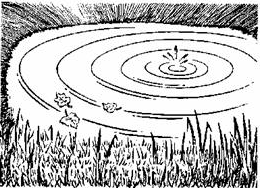
\includegraphics[width=\linewidth]{acoustics/lake.png}
    \captionof{figure}{%
    Imagine a calm pool. The surface is flat and smooth. Drop a rock into it. Kerploop. The surface is now disturbed.
    The disturbance spreads propagates, as well know waves. The medium here is the water surface.
    }
    \label{fig:acoustics:lake}
}
The propagation happens at a certain speed which depends on the physical properties of the medium, such as its density and composition.
The medium assumed through out the entire thesis is air.
Under the fair assumption of air being homogeneous and steady,
the speed of sound can be computed with the following approximated formula:
\begin{equation}
    \cair =  331.4 + 0.6\temperature + 0.0124\rhumidity \hspace{1em} [\sfrac{\si{\metre}}{\si{\second}}]
    ,
\end{equation}
where $\temperature$ is the air temperature $[\si{\celsius}]$ and $\rhumidity$ is the relative air humidity $[\%]$.
The changes in air pressure can be represented by a \textit{waveform}, which is a graphic representation of a sound.

\begin{figure}[h]
    \centering
    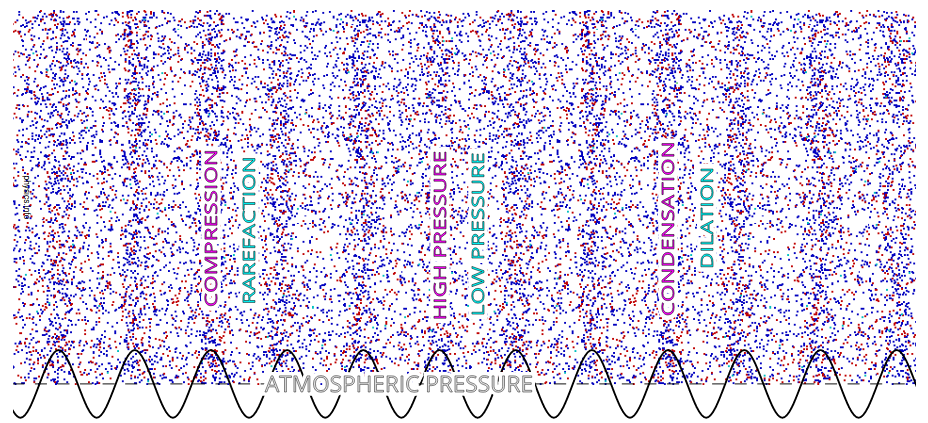
\includegraphics[width=\linewidth]{acoustics/acoustic_wave.png}
    \caption{snapshot of a longitudinal wave in air}
    \label{fig:acoustics:acoustics_wave}
\end{figure}
In general, the sound field is complex which can be decomposed as a superimposition of several waves~\cite{kuttruff2016room}.

We think at this process in the light of the classic \textit{source-medium-receiver} model of communication theory.
\begin{description}
    \item[source] is anything that emits or expends energy (waves)
    \sidenote{%
    example of sources are vibrating solids (\eg/ speakers membrane),
    rapid compression or expansion (\eg/ explosions or implosions)
    or air vortices with characteristics frequencies (\eg/ flute and whistles).
    },
    \item[medium] is the vehicle for carrying waves from one point to another, and
    \item[receiver] absorbs the such waves.
\end{description}

The behavior of acoustic waves is defined by the acoustic-wave equation.
The rest of the section is reproduce the derivation of this equation, re-arranging the derivation presented in \cite{kuttruff2016room, pierce2019acoustics, marczuk2006modelling, avanzini2019sound}.

\subsection{The Acoustic wave equation}\label{subsec:acoustics:waveq}
It is a second-order partial differential equation
\sidenote{
    In 1746, d’Alembert discovered the one-dimensional wave equation for music strings,
    and within ten years Euler discovered the three-dimensional wave equation for fluids.
} which describes the evolution of acoustic pressure $\pressure$
as function of the position $\positionMicrophone$ $[\si{\metre}]$ and time $t$ $[\si{\second}]$
\marginpar{%
    \footnotesize
    The symbol $\knabla^2 = \kpderiv[2]{}{x} + \kpderiv[2]{}{y} + \kpderiv[2]{}{z}$
    stands for the 3-dimensional \textit{Laplacian} operator.
}
\begin{equation}
    \label{eq:acoustics:wave}
    \knabla^2 \pressureSpaceTime - \frac{1}{\speedOfSound^2} \kpderiv[2]{\pressureSpaceTime}{t} = 0
    .
\end{equation}
The constant $\speedOfSound$ is the sound velocity in the medium with dimension $[\frac{\si{\metre}}{\si{\second}}]$.

Assuming the propagation of the wave in a homogeneous medium, one can obtain the equation above by combining three fundamental physical laws:
\begin{itemize}
    \item the \textit{conservation of momentum}\sidenote{In fluidodynamics, it comes with the name of the Euler's equation},
    \item the \textit{conservation of mass}, and
    \item the \textit{polytropic process relation}\sidenote{meaning that the medium is an ideal gas undergoing a reversible adiabatic process}.
\end{itemize}

In general medium are not uniform and features inhomogeneities of two types:
scalar inhomogeneities, \eg/ due to temperature variation,
and vector inhomogeneities, \eg/ due to presence of fans or air conditioning.
Although these affect the underlying assumption of the model, the effect are small in typical application of speech and audio signal processing.
Therefore they are commonly ignored.

\newthoughtpar{The Helmholtz's equation}
The wave equation~\ref{eq:acoustics:wave} is expressed in the space-time domain $\depSpaceTime$.
By applying the temporal Fourier transform, we obtain the \textit{Helmholtz equation}, \ie/
\begin{equation}
    \label{eq:acoustics:helmholtz}
    \knabla^2 P(\positionMicrophone, f) + k^2 P(\positionMicrophone, f) = 0
    ,
\end{equation}
where $k = \frac{2 \pi f}{c}$  is known as \textit{wave number} $[\si{\metre^{-1}}]$, that relates the frequency $f \; [\si{\hertz}]$ and the propagation velocity $c$.

Both the wave equation~\ref{eq:acoustics:wave} and the Helmholtz's equation~\ref{eq:acoustics:helmholtz} are source independent,
namely no source is present in the medium.
Therefore they are called \textit{homogeneous} as the right-hand term is zero.

Normally the sound field is a complex field generated by acoustics sources.
As consequence, the two equation becomes inhomogeneous as some non-zero terms needs to be added to the right-hand sides.

In presence of a sound source producing waves with distribution function $s(t, \positionMicrophone)$, the wave equation can be written
\begin{equation}
    \label{eq:acoustics:source}
    \knabla^2 \pressureSpaceTime - \frac{1}{\speedOfSound^2} \kpderiv[2]{\pressureSpaceTime}{t} = s(t, \positionMicrophone)
    .
\end{equation}
Then, the correspondent Helmholtz's equation writes
\begin{equation}
    \label{eq:acoustics:source_freq}
    \knabla^2 P(\positionMicrophone, f) + k^2 P(\positionMicrophone, f) = - S(\positionMicrophone, f)
    .
\end{equation}

For instance one can assume an infinitesimally small pulsating sphere locate at $\positionSource$ radiating constant acoustic energy at frequency $f$,
\ie/ $S(\positionMicrophone) = \delta(\positionMicrophone - \positionSource)$.
At the receiver position $\positionMicrophone \neq \positionSource$, the Helmholtz's equation writes
\begin{equation}
    \label{eq:acoustics:green_definition}
    \knabla^2 H(f, \positionMicrophone \mid \positionSource)
     + k^2 H(f, \positionMicrophone \mid \positionSource) = - \delta(\positionMicrophone - \positionSource)
    ,
\end{equation}
The function $H(f, \positionMicrophone \mid \positionSource)$ that satisfy \cref{eq:acoustics:green_definition} is the \textit{Green's function}
associated to ~\cref{eq:acoustics:helmholtz}, for which is also a solution.
\\In the next subsection, we will see that the function $H$ can be interpreted as the free-field \textit{Transfer Function}
between the source at $\positionSource$ and the receiver at $\positionMicrophone$.

\subsection{... and its solution as Green's function}
\marginpar{%
    \footnotesize
    By 1950 Green’s functions for Helmholtz’s equation were used to find the
    wave motions due to flow over a mountain  and in acoustics.
    Green’s functions for the wave equation lies with Gustav Robert Kirchhoff (1824–1887),
    who used it during his study of the three-dimensional wave equation.
    He used this solution to derive his famous \textit{Kirchhoff’s theorem}~\citeonly{duffy2015green}.
}
\textsc{The Green's Functions} are mathematical tools for solving linear differential equations with specified initial- and boundary- conditions~\cite{duffy2015green}.
They have been used to solve many fundamental equations, among which \cref{eq:acoustics:helmholtz,eq:acoustics:wave} for both free and bounded propagation.
\begin{center}
    \textit{
    They can be seen as the equivalent concept of the
    \\ \emph{impulse responses
    \sidenote{impulse response in time domain, trasfer fuction in the frequency domain.}}
    used in signal processing.}
\end{center}
Under this light the physic so-far can be rewritten in the vocabulary of the communication theory, namely \textit{input}, \textit{filter} and \textit{output}.

According to Green's method, the equations above can be solved in the frequency domain for arbitrary source as follows:
\marginpar{%
    \footnotesize
    If one ignores the space integal, one can see the close relation with a transfer function.
}
\begin{equation}
    \label{eq:acoustics:helmholz_conv}
    P(f, \positionMicrophone) = \iiint_{\volume_\contSource} H(f, \positionMicrophone \mid \positionSource) S(f, \positionSource) \kdiff\positionSource
    ,
\end{equation}
where $\volume_\contSource$ denotes the source volume,
and  $\kdiff\positionSource =  \kdiff{x_\contSource}\,\kdiff{y_\contSource}\,\kdiff{z_\contSource}$ the  differential  volume element at position $\positionSource$.
\\The requested sound pressure $\pressureSpaceTime$ can now be computed by taking the frequency-directional inverse Fourier transform of \cref{eq:acoustics:helmholz_conv}.

It can be shown \citeonly{kuttruff2016room} that the Green's function for~\cref{eq:acoustics:helmholtz,eq:acoustics:green_definition} writes
\begin{equation}
    \label{eq:acoustics:greenFreeFreq}
    H(f, \positionMicrophone \mid \positionSource) = \frac{1}{4 \pi \norm{\positionMicrophone - \positionSource}} e^{- \frac{\Ii 2 \pi f \norm{\positionMicrophone - \positionSource}}{\speedOfSound}}
\end{equation}
where $\norm{\cdot}$ denotes the Euclidean norm.
\marginpar{
    \footnotesize
    \cref{eq:acoustics:greenFreeFreq,eq:acoustics:greenFreeTime} are respectively the free-field transfer function and the impulse response.
}
By applying the inverse Fourier transform to the result above, we can write the time-domain Green's function as
\begin{equation}
    \label{eq:acoustics:greenFreeTime}
    h(t, \positionMicrophone \mid \positionSource) =
        \frac{1}{4 \pi \norm{\positionMicrophone - \positionSource}}
        \diracOf{t - \frac{\norm{\positionMicrophone - \positionSource}}{\speedOfSound}}
\end{equation}
where $\diracOf{\cdot}$ is the time-directional Dirac delta function.
\\As a consequence, the \textit{free field}, that is in open air without any obstacle, the  sound propagation
incurs a delay $\distMicSrc / c$
and an attention $1 / (4 \pi \distMicSrc)$ as function of the distance
$ \distMicSrc = \norm{\positionMicrophone - \positionSource}$ from source to the microphone.

According to \cref{eq:acoustics:greenFreeTime}, the sound propagate around a point source with a spherical pattern.
When the receiver is far enough from the source, the curvature of the \textit{wavefront} may be ignored.
The waves can be approximated as \textit{plane waves} orthogonal to the propagation direction.
This scenario depicted in \cref{fig:acoustics:planewaves} is known as \textit{far-field}.
\marginpar{%
    \centering
    \footnotesize
    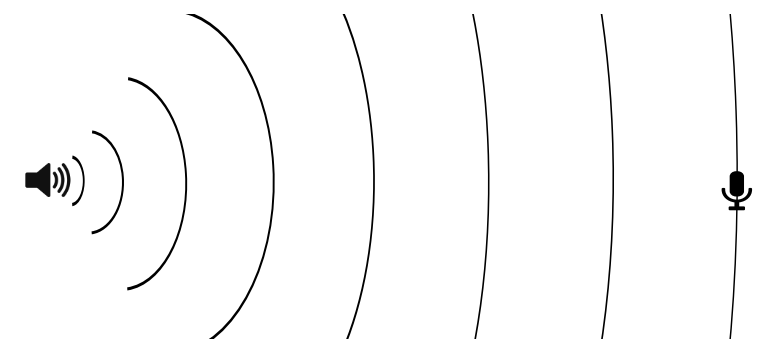
\includegraphics[width=\linewidth]{acoustics/planewaves.png}
    \captionof{figure}{%
    Visualization of the sound propagation. Since the sensor (i.e. a microphone)
    is drawn in the far field, the incoming waves can be approximated as plane waves.
    }
    \label{fig:acoustics:planewaves}
}
As opposed to, when the distance between the source and the receiver is small, the scenario is called \textit{near field}.

%%%%%%%%%%%%%%%%%%%%%%%%%%%%%%%%%%%%%%%%%%%%
\section{Acoustic Reflections}\label{ch:acoustics:sec:reflection}
The equations derived so far assumed unbounded medium, \ie/ free space: a rare scenario in everyday applications.
Real mediums are typically bounded, at least partially.
For instance in a room, the air (propagation medium) is bounded by walls, ceiling, and floor.
When sound travel outdoor, the ground acts as a boundary for one of the propagation direction.
Therefore, the sound wave does not just stop when it reaches the end of the medium or when it encounters an obstacle in its path.
Rather, a sound wave will undergo certain behaviors depending on the obstacle acoustics and geometrical properties, including
\begin{itemize}
    \item \textit{reflection} off the obstacle,
    \item \textit{diffraction} around the obstacle,
    \item and \textit{transmission} into the obstacle, causing
    \begin{itemize}
        \item \textit{refraction} though it, and
        \item \textit{dissipation} of the energy.
    \end{itemize}
\end{itemize}

\marginpar{%
    \centering
    \footnotesize
    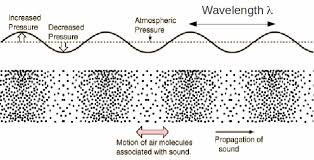
\includegraphics[width=\linewidth]{acoustics/wavelength.jpg}
    \captionof{figure}{%
        wavelength
    }
    \label{fig:acoustics:wavelength}
}
In order, reflections arise typically when a sound wave hit a large surface, like a room wall.
When the sound meets a wall edge or a slit, the wave diffracts, namely it bends around the corners of an obstacle.
The point of diffraction effectively becomes a secondary source which may interact with the first one.
\\The part of energy transmitted to the object may be absorbed and refracted.
Object are characterized by a proper acoustic resistance, called \textit{acoustic impedance}, which
describes its acoustic inertia as well as the energy dissipation.
The remaining contribution may continue to propagate causing resulting in the refraction phenomenon \sidenote{%
    This is more commonly observed when light pass thought different medium, like a prism.
}.

\textsc{When sound reflects} on an solid surface, two type of acoustic reflection can occurs: part of the sound energy
\marginpar{%
    \centering
    \footnotesize
    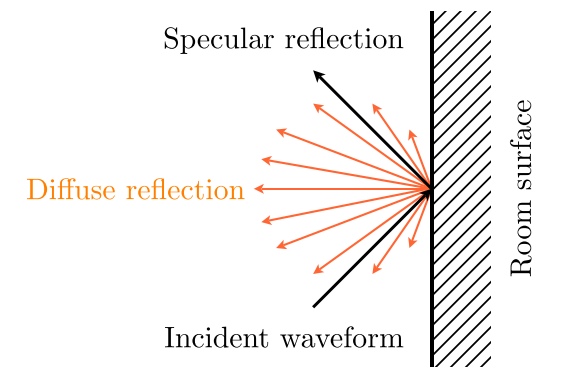
\includegraphics[width=\linewidth]{acoustics/reflection.png}
    \captionof{figure}{%
        Specular vs diffuse reflection
    }
    \label{fig:acoustics:reflection}
}
\begin{itemize}
    \item is reflected \textit{specularly}, \ie/, the angle of incidence equals the angle of reflection; and
    \item is reflected \textit{diffusely} - or \textit{scattered}, \ie/, scatter in every direction).
\end{itemize}

All the phenomena occurs with different proportions depending on the acoustics and geometrical properties of surface and the frequency content of the wave.
In acoustics, it is common to define the \textit{operating points} and different \textit{regimes}\sidenote{for instance near- vs. far-field}
according to the sound frequencies or the correspondent \textit{wavelength} $[\si{\metre}]$,
\begin{equation}
    \wavelength = \frac{2 \pi}{k} = \frac{\speedOfSound}{f} \hspace{1em} [\si{\metre}]
    ,
\end{equation}
where $f$ is the frequency of the sound wave.

\marginpar{
    \footnotesize
    \textit{Sabine had previously used ray-based acoustics in the
    early 1900s to investigate sound propagation paths using Schlieren photography.
    Their impressive visualizations show wavefronts that are augmented
    with rays that are perpendicular to the wavefronts.}
    \\---\citeauthor{savioja2015overview}
}
As depicted in~\cref{fig:acoustics:wavelength}, $\wavelength$ measures the spatial distance between two molecules in the medium having the same value of pressure.
% \marginpar{%
%     \footnotesize
%     a frequency of $\SI{1}{\kHz}$ corresponds to a wavelength of approximately $\SI{34}{\cm}$ ,
%     which is one or two orders of magnitude smaller than typical linear dimensions of rooms,
%     as well as typical distances traveled by sound waves in a room
% }.
\marginpar{
    \centering
    \footnotesize
    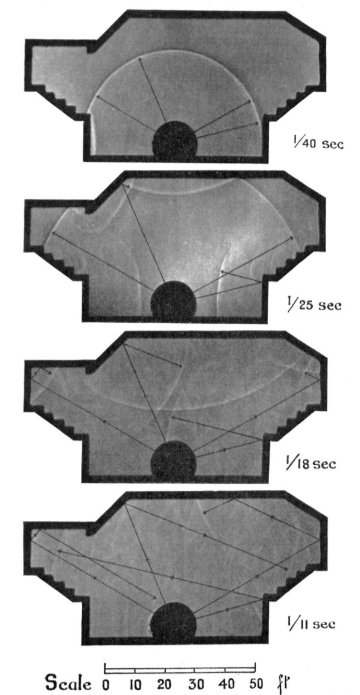
\includegraphics[trim={0 205 0 0},clip,width=\linewidth]{acoustics/sound_pulse1926.png}
    \captionof{figure}{%
        Photographs showing successive stages in the progress of a Sound Pulse in a Model Section of a Debating Chamber.
        \imgsrc{\citeonly{davis1926sound}}
    }
    \label{fig:acoustics:reflection}
}
\\Using this quantity we can identify the following three response of the objects (irregularities) of size $d$ to a plane-wave depicted in~\cref{fig:acoustics:irregularities}
\begin{figure}
    \footnotesize
    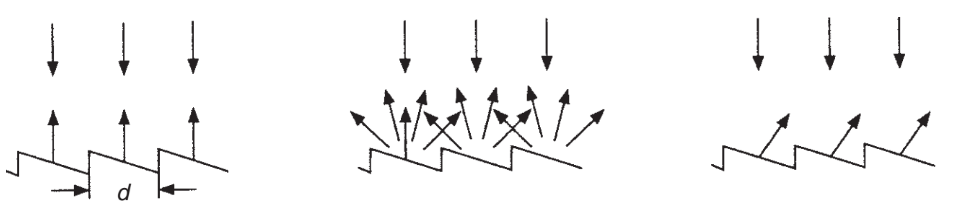
\includegraphics[width=\linewidth]{acoustics/irregularities.png}
    \captionof{figure}{%
        A reflector having irregularities on its surface with width $d$ much smaller than the sound wavelength $\wavelength$.
        Image courtesy of \citeonly{kuttruff2016room}.
    }
    \label{fig:acoustics:irregularities}
\end{figure}
\begin{itemize}
    \item $\wavelength \gg d$, the irregularities are negligible and the sound wave reflection is of specular type;
    \item $\wavelength \approx d$, the irregularities break the sound waves which is reflected towards every direction;
    \item $\wavelength \ll d$, each irregularities is a surface reflecting specularly the sound waves.
\end{itemize}

\textsc{All this presented behavior} can be described with the wave equation imposing opportune boundary conditions.
% However working with this formula might results complicated and difficult.
A simplified yet effective approach - just as in optics - is to model incoming sound waves as \textit{acoustic rays}~\citeonly{davis1926sound, krokstad1968calculating}.
A ray has well-defined direction and velocity of propagation, and conveys a total wave energy which remains constant.
This simplified description undergoes with the name of \GAdef/~\cite{savioja2015overview}, and share many fundamentals with geometrical optics.
This model will be convenient to describe and visualize the reflection behavior hereafter.

\subsection{Large smooth surfaces, absorption and echoes}
% The main focus of this section and the this whole thesis goes on \textit{specular reflections}.
Specular reflection are generated by surfaces which can be modelled as infinite flat, smooth and rigid (\ie/ stationary).
As mentioned above, this assumption is valid as long as the surface has dimension much bigger than the sound wavelength.
Here the acoustic ray is reflected according to the \textit{law of reflection}, stating that
(i) the reflected ray remains in the plane identified by the incident ray and the normal to the surface,
and (ii) the angles of the incident and reflected rays with the normal are equal.
\marginpar{%
    \centering
    \footnotesize
    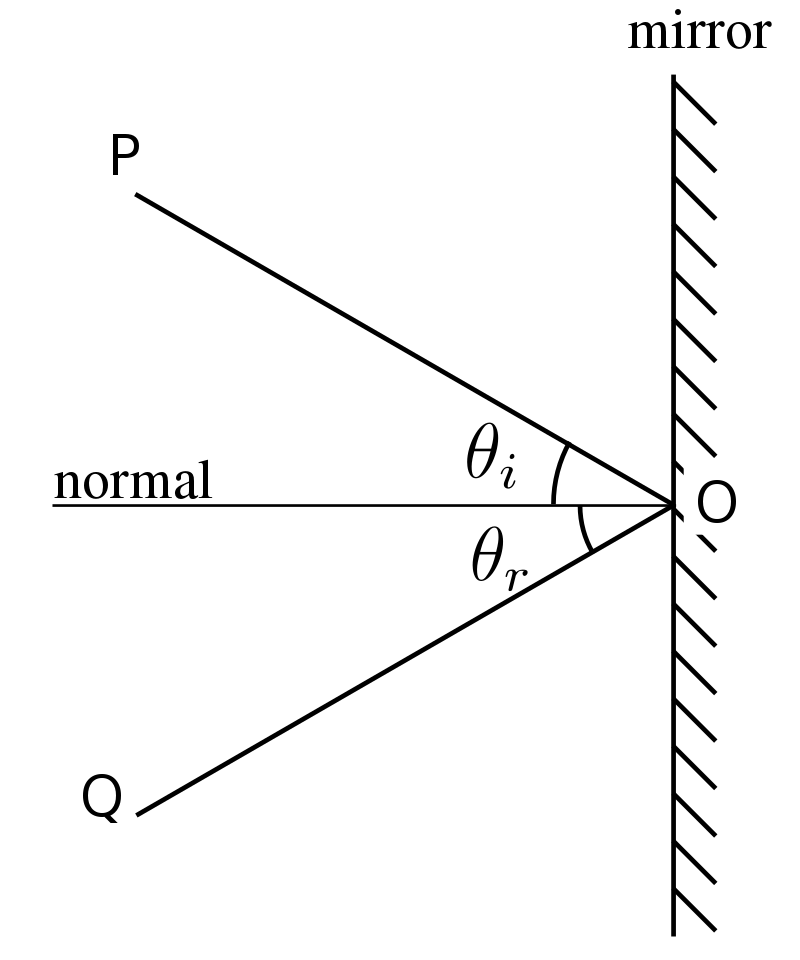
\includegraphics[width=\linewidth]{acoustics/reflection_law.png}
    \captionof{figure}{%
        Specular reflection
    }
    \label{fig:acoustics:reflection_law}
}

If the surface $\surface$ is not perfectly rigid or impenetrable, its behavior is described by the \textit{acoustic impedance}, $\impedence_\surface(f) \in \bbC$.
%\sidenote{\textbf{acoustic impendence} measures the opposition that an acoustic system presents to the acoustic pressure}.
Analytically, it is defined as relation between sound pressure and particle velocity at the boundary.
It consists of a real and imaginary part, called respectively acoustic \textit{resistance} and \textit{reactance}.
The former can be seen as the part where energy is lost, while the latter as the part where energy is stored.
% It measures the portion of energy absorbed by the surface and the incident acoustic wave.
% describes the relation between pressures of the incident arriving waveform and the reflected wave

\newthought{The reflection coefficient} $\reflCoeff$ can be derived by the acoustic impedance
for plane waves, \ie/ under assuming a far-field regime between source, receiver and surface,.
\begin{center}
    \textit{It measures the portion of energy absorbed by the surface
    \\and the incident acoustic wave.}
\end{center}
Analytically, it is defined as  \cite{kuttruff2016room,pierce2019acoustics}
\begin{equation}
    \reflCoeff(f, \theta) = \frac{\impedence_\surface(f)\cos{\theta} - \impedenceAir(f)}{\impedence_\surface(f)\cos{\theta} + \impedenceAir(f)}
    ,
\end{equation}
where $\impedence_\surface(f)$ and $\impedenceAir(f)$ are the frequency-dependent impedance of the surface and the air respectively,
and $\theta$ is the angle of incidence.

\textsc{The absorption coefficient} is typically used instead in the context of \GA/ and the audio signal processing.
It comes from following approximations~\citeonly{savioja2015overview}.
(i) The energy or intensity of the plane wave\sidenote{%
    since it is the square magnitude of the acoustic pressure, the phase information is lost.
}, is considered instead of the acoustic pressure;
(ii) dependency on the angle of incidence is relaxed in favor of the averaged quantities;
(iii) local dependency on frequencies is relaxed in favor of a frequency-independent scalar or at most a description per octave-band.
This assumption are motivated by the difficulty of measuring the acoustic impedance
and the possibility to compute an equivalent coefficient a posteriori

Therefore, it is customary to use the absorption coefficient, defined as
\begin{equation}
    \absCoeff(f) = 1 - \abs{\bar{\reflCoeff}(f)}^2
    ,
\end{equation}
where $\bar{\reflCoeff}$ is the reflection coefficient averaged over the angles $\theta$.

\marginpar{%
    \footnotesize
    The word echo derives from the Greek 'echos', litterarly ``sound''.
    In the folk story of Greek, Echo is a mountain nymph whose ability to speak was cursed:
    she only able to repeat the last words anyone spoke to her.
}\newthought{Echoes are specular reflections} which stand out in terms of energy strength or timing~\citeonly{kuttruff2016room}.
Originally this term used to indicate sound reflections which are subjectively noticeable as a separated repetition of the original sound signal.
These can be heard consciously in outdoor scenario, such as in mountain. However, they are less noticeable to the listener in close rooms.
In~\cref{ch:acoustics:subsec:rir} a proper definition of echoes will be given with respect the temporal distribution of the acoustic reflection.



\subsection{Diffusion, Scattering and Diffraction of Sound}
Real-world surfaces are not ideally flat and smooth; they are rough and uneven.
Examples of such surfaces are coffered ceilings, faceted walls, raw brick walls as well as the entire audience area of a concert hall.
When such irregularities are in same order of the sound wavelength, \textit{diffuse reflections} is observed.

In the context of \GA/, the acoustic ray associated to a plane-wave can be though as a bundle of rays traveling parallel.
When it strikes such a surface, each individual rays are bounced off irregularly, creating \textit{scattering}:
a number of new rays are created, uniformly distributed in the original half-space.
The energy carried by each of the outgoing ray is angle dependent and it
is well modeled thought the \textit{Lambert's cosine law}, originally used to describe optical diffuse reflection.

The total amount of energy of this reflection may be computed a-priori
knowing the \textit{scattering} coefficient proper of the surface material.
Alternatively, it can be derived a-posteriori with the \textit{diffuse coefficient}, namely the ratio between
the specularly reflected energy over the total reflected energy.

\textit{Diffraction waves} occurs when the sound confronts the edge of a finite surfaces, for instance around corners or through door openings.
This effect is show in~\cref{fig:acoustics:diffraction}
\marginpar{%
    \centering
    \footnotesize
    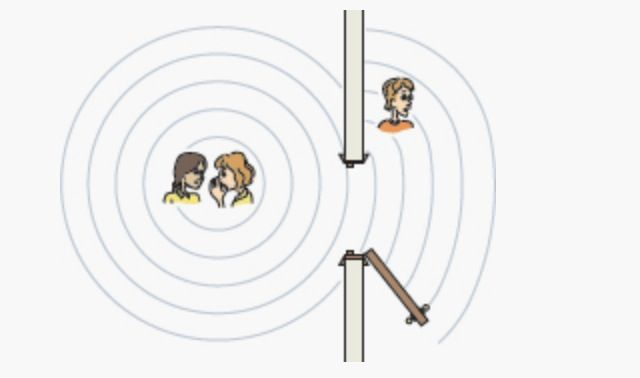
\includegraphics[width=\linewidth]{acoustics/sound_diffraction.jpg}
    \captionof{figure}{%
        Sound Diffraction effect.
    }
    \label{fig:acoustics:diffraction}
}
At first the sound wave propagates spherically from the source.
Once it reaches the reflector with apertures, the wave is diffracted, \ie/ bended, behind it.
It is interesting to note that the diffraction waves produced by the semi-infinite reflector edge
allow the area that is ``behind'' the reflector to be reached by the propagating sound.
This physical effect is exploited naturally by the human auditory system to localize sound sources.

% -----------------------------------------------------------------------------

\section{Room Acoustics and Room Impulse Response}\label{ch:acoustics:sec:rir}
Room acoustics concerns with acoustic waves propagating in air enclosed in a volumes with a set of surfaces
(walls, floors, etc.), from which an incident wave may be interact as described in \cref{ch:acoustics:sec:reflection}.
In this context, a
\begin{center}
    \textit{\emph{room} is a physical enclosure containing the medium and has boundaries limit the sound propagation.}
\end{center}

\textsc{Mathematically} the sound propagation is described by the wave equation~\eqref{eq:acoustics:wave}.
By solving it, the \AIRdef/\sidenote{\ATFdef/ in the Fourier transform of the \AIR/}
from a source to a microphone can be obtained.
In the context of room acoustics, it is commonly referred to as \RIRdef/, usually to put attention of
on the geometric relation between reflections and the geometry of the scene.
In this thesis the two terms will be used indistinctly.

\subsection{The Room Impulse Response}\label{ch:acoustics:subsec:rir}
It is a fundamental concept of this dissertation and it is where physical room acoustic
(Green's function/Solution of wave equation) and indoor audio signal processing meets.
From now on, we well adopt an signal processing perspective and
\begin{center}
\textit{The \RIR/ is a causal time-domain filter that accounts for the whole indoor sound propagation
from a source to a receiver}
\end{center}
\cref{fig:acoustics:rir} provides a schematic illustration of the shape of a \RIR/ in comparison with measured one.
\begin{figure}[h]
    \centering
    \begin{minipage}[b]{.5\textwidth}
        \centering
        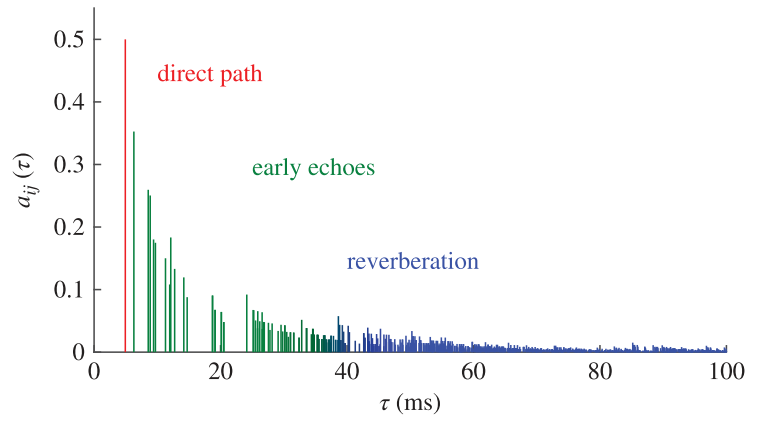
\includegraphics[width=\linewidth]{acoustics/rir_schematic.png}
    \end{minipage}%
    \begin{minipage}[b]{.5\textwidth}
        \centering
        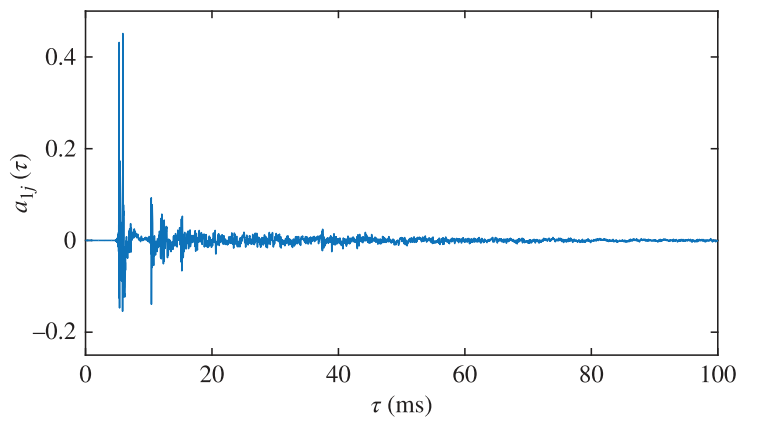
\includegraphics[width=\linewidth]{acoustics/rir_measured.png}
    \end{minipage}
    \caption{Schematic illustration of the shape of an \RIR/ and the first 100 ms of a measured one.}
    \label{fig:acoustics:rir}
\end{figure}

\RIRs/ usually exhibits common structure.
Based on the consideration in~\cref{ch:acoustics:sec:reflection},
they are commonly divided into three components \citeonly{kuttruff2016room}:

\begin{equation}\label{eq:acoustics:rir_full}
\rir(t) = h^d(t) + h^e(t) + h^l(t)
,
\end{equation}
where
\begin{description}
    \item[Direct path] $h^d(t)$ is the line-of-sight contribution of the sound wave.
    This term coincides with the spike modeled by the free-field propagation\sidenote{\cfr{The free-field Green's function, \ie/~\cref{eq:acoustics:greenFreeTime})}}.
    \item[Echoes or Early Refelction] are included in $h^e(t)$ comprising few disjoint reflections coming typically from room surfaces.
    They are usually characterized by sparsity in the time domain and greater prominence in amplitude.
    This first reflections are typically specular and are well modeled in general by the \ISM/\sidenote{\cfr{\cref{subsec:acoustics:ism}}}.
    \item[Later Reverberation] or simply \textit{reverberation} $h^l(t)$ collects many reflections occurring simultaneously.
    This part is characterized by a diffuse sound filed with exponentially decreasing energy.
\end{description}
This three components are not only ``visible'' when plotting the \RIR/ against time,
but they are characterized by different perceptual features, as explained~\cref{ch:acoustics:sec:perception}.

To conclude with, let $s(t)$ be the source signal, sound received is
\begin{equation}
    x(t) = (\rir \conv s)(t)
    ,
\end{equation}
where the symbol $\conv$ is the convolution operator.

A part for certain simple scenarios, computing \RIRs/ in closed forms is a cumbersome task.
Therefore numerical solver or approximation model are used instead.

\subsection{Simulating Room Acoustics}\label{sec:acoustics:simulators}
There are two main categories: geometric and wave-based methods~\cite{habets2006room, savioja2015overview}.
\begin{description}
    \item[wave-based] aims at solving the wave equation numerically, while
    \item[geometric] methods make some simplifying assumption about the wave propagation:
    they typically ignore the \textit{wave} behavior of the sound, choosing much lighter models such as \textit{ray}s or \textit{particle}s.
\end{description}

\newthoughtpar{Wave-based Methods}.
% description
These are iterative methods that divide the 3D bounded enclosure into a grid of interconnected nodes
--- mechanical unit with simple degree of freedoms.
For instance, the
\FEMf/ divide the space into small volume elements smaller of the sound wavelengths, while
\BEMf/ divide only the boundaries of the space are divided into surface elements.
These nodes interact with each other according to the math of the wave equation.
Unfortunately, at high frequencies, the elements must be very small, so their number increases, so the computational complexity increases.
This methods allow to create grid with denser interconnection where required.
\\The \FDTDf/ method replace the derivatives in the wave equation, with its discrete approximation, \ie/ finite differences.
The space is divided into a regular grid, where the changes of a quantity (air pressure or velocity) is computed over time at each grid point.
\DWMf/ methods are a subclass of \FDTD/ often used in acoustics problem.

\begin{figure}[t]
    \label{fig:acoustics:fdtd}
    \centerfloat
    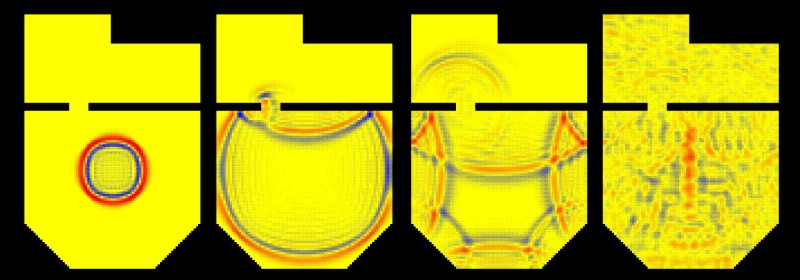
\includegraphics[width=.8\paperwidth]{acoustics/simulator_dwg.jpg}
    \caption{Simulation of Sound propagation at four consecutive timestamps using the \DWM/ technique.
    A short, sharp, impulsive sound fired into the larger of two rooms causes a circular wavefront to spread out from the sound source.
    The the wave is reflected from the walls and part of it passes through a gap into the smaller room.
    In the larger room, interference effects are clearly visible;
    in the smaller room, the sound wave has spread out into an arc, demonstrating the effects of diffraction.
    A short while after the initial event, the sound energy has spread out in a much more random and complex fashion.
}
\end{figure}

\begin{figure}[t]
    \label{fig:acoustics:fdtd}
    \centering
    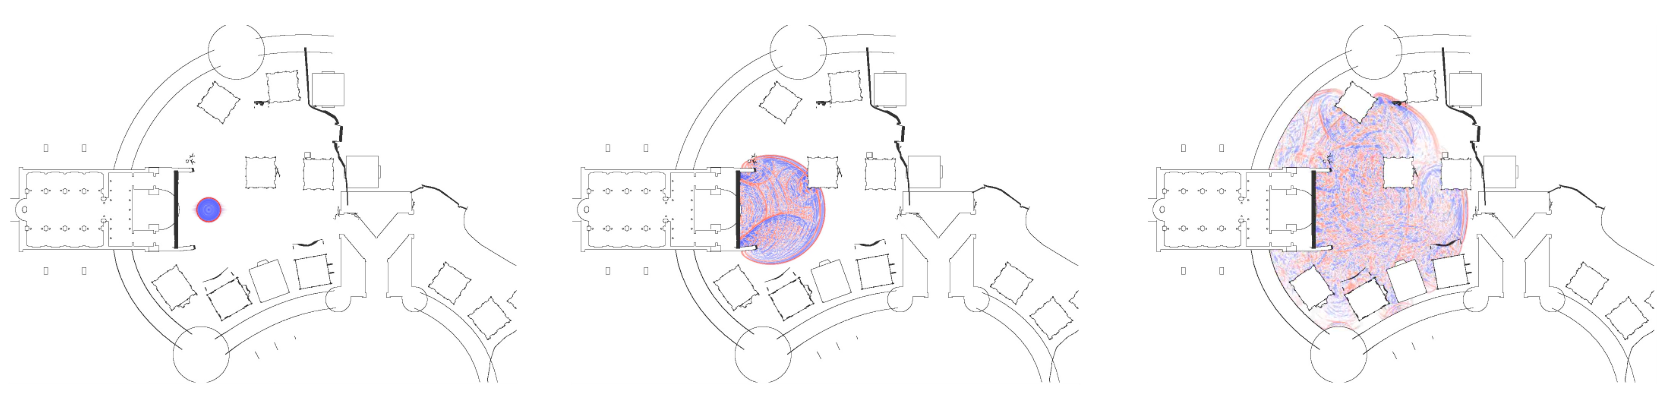
\includegraphics[width=\textwidth]{acoustics/wave-simulation_fdtd.png}
    \caption{Sound propagation at three consecutive timestamps using the \FDTD/-based \textit{Triton} simulator from Microsoft}
\end{figure}

\textsc{The main drawback of these methods} is  discretisation problem:
less dense grid may simplify too much the simulation, while denser grid increase the computational load.
Moreover, in order to achieve good simulation, their require delicate definitions of the boundaries condition and
their complex impedances, parameters not always available in the literature.
\\\textsc{On the other hand} these methods inherently account for many effects such as reflection, diffusion, diffraction and interferences.
In particular by simulating the low-frequencies components of the \RIR/, they are able to well approximate \textit{room modes}
\sidenote{
    Room modes have the effect of amplifying and attenuating specific frequencies in the \RIR/,
    and produce much of the subjective sonic ``colour'' of a room.
}
Reproducing and studying modes is of vital importance
for evaluating acoustic of rooms, such as concert hall, and recording studios or when producing musically pleasing reverbs.

Above all, \DWMf/ are usually preferred\cite{valimaki2016more}: they run directly in the time domain, requiring easier implementation;
and they exhibits a natural huge level of parallelism
\sidenote{each individual node in the grid
(in number of thousands or millions) can be updated without synchronization,
leading to an massive computational reduction}.

\newthoughtpar{Geometric metods}
\marginpar{For a detailed discussion about geometric acoustic methods, please refer to \cite{Savioja2015goemetric}}
They can be grouped into \textit{stochastic} and \textit{deterministic} approaches.
They typically compute the reflection path(s) between the source and the receivers,
assuming that the wave behaves like a particles and a ray carrying the acoustic energy around the scene.

\newthought{Stochastics} are approximate by nature.
They are based on statistical modeling of the \RIRs/ or approximation via Monte Carlo methods.
The formers writes statistical signal processing models based on prior knowledge,
such as energy envelopes and probability distribution of the \RIR/ in regions of time-frequency domain  \cite{Badeau2019common}.
The latters randomly and repeatedly subsample the problem space, recording samples which fulfil some correctness criteria, and discarding the rest.
By combining the results from multiple samples, the probability of an incorrect result is reduced, and the accuracy is increased.
Typically the trade-off between quality and speed is straightforwardly adjusted by choosing the number of samples.

The most common is the \textit{ray-tracing}\cite{Kulowski1985algorithmic} or \textit{diffuse rain}\cite{Schroeder2007fast, Heinz1993binaural, Wabniz2010}

\newthought{Ray-tracing}.
Modeling of waves as discrete particles.
Great success in the field of computer graphics for modeling reflection of light.
The assumption that rays and waves are interchangeable is good for high frequencies.
For low frequencies, where the wavelength are of the same order of the wall surface, it may leads to strong approximation error:
interferences and diffractions effects are not taken into account at these frequencies\cite{Savioja2015goemetric}.

This simulation technique models the propagation by a series of discrete rays that are traced around the room.
Each ray trajectory is reflected in a random direction every time it hits a wall and its energy is scaled according to the wall absorption, air absorption and distance attenuation).
The process of tracing a ray is continued until the ray’s energy falls below a predefined threshold.
At each reflection, the ray's energy over frequency, its time and angle of arrival are recorded in histogram, namely a
\textit{directional time-frequency-energy map} of the room’s diffuse sound field for a giver receiver location.
This map is then used as prior distribution for drawing random set of impulses which are used to form the \RIR/.

\newthought{Deterministic} methods.
the most popular is the Allen and Barkley's \ISMf/\cite{allen1979image}.
It accurate traces the exact direction and the timing of the main reflections' paths.

For a 3D shoebox with rigid walls, it is able to produce an exact solution to the wave equation.
It models only specular (perfect) reflections, ignoring diffuse and diffracted components.
For this is only approximate inexactly arbitrary enclosures and the late reflections, which is predominantly diffuse.

The naive implementation reflects the sound source against all surfaces in the scene, resulting in a set of image sources. Then, each of these image sources is itself reflected against all surfaces
For these reasons, the image-source method is only suitable for early reflections, and is generally combined with a stochastic method to find the late part of an impulse response
For higher order of reflection (\~20), the algorithmic complexity explodes becomes impractical.
For these reasons, the image-source method is only suitable for early reflections, and is generally combined with a stochastic method to find the late part of an impulse response (IR).

\newthought{Hybrid Methods}
As discussed above, the image-source method is accurate for early reflections, but slow for longer responses.
The ray tracing method is by nature an approximation, but produces acceptable responses for diffuse field.
The waveguide method models physical phenomena better than the geometric methods, but is expensive at high frequencies.
This limitation corresponds into three regions in the Time-Frequency representation of the \RIR/.
As depicted in~\cref{fig:acoustics:rir_regions},
\begin{itemize}
    \item in the time domain, a transition can be identified between the early vs. late reflection, corresponding to the validity of the deterministic vs. stochastic models;
    \item and in the frequency domain, between geometric and wave-based modeling.
\end{itemize}

By combining all three models, accurate broadband impulse responses can be created,
but for a much lower computational cost than would be possible with any individual method.
However, this is possible provided that the time- and frequency-domain
\textit{crossover point} are respected and the level of each component is scaled accordingly.

\marginpar{%
    \centering
    \footnotesize
    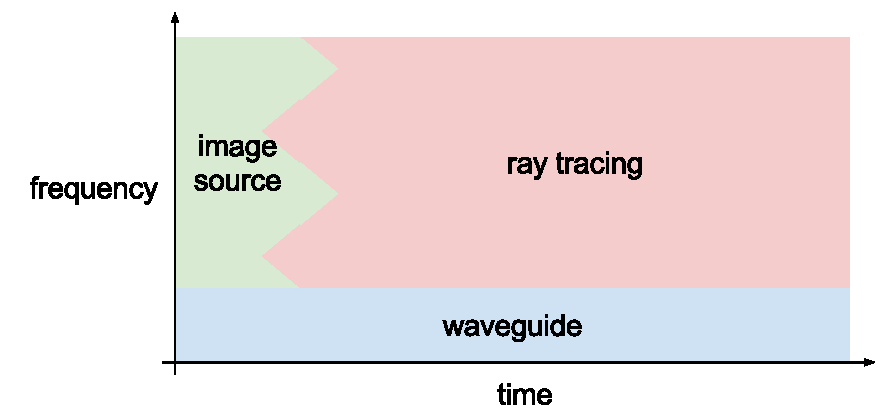
\includegraphics[width=\linewidth]{acoustics/rir_regions.pdf}
    \captionof{figure}{%
    Time-Frequency profile of reverberation Adapted from \cite{Badeau2019common, Wayverb}.
    }
    \label{fig:acoustics:rir_regions}
}

The crossover point in the time domain is called \textit{transition time} or \textit{mixing time}.
It identifies the moment after which reflections are so frequent that they form a continuum and, because the sound is partially absorbed by the room surfaces at every reflection, the sound level decays exponentially over time \cite{Badeau2019common}
This point define the cross-fade between the deterministic and the stochastic process.
Notice, that the latter will record both specular and diffuse reflections.

The crossover point in the frequency domain is called \textit{Schroeder's frequency}, splitting the
spectrum of the \RIR/ into a region with a few isolated modes and one where they can be threated as a
continuous random process, called respectively the \textit{resonant} and \textit{even} behaviors.
This point define the cross-fade between the geometrical and wave-based model.

Each simulator has its own way to compute and implement this crossover points.

\subsection{The Method of Images and the Image Source Model}\label{subsec:acoustics:ism}

The \textit{Method of Images} is a mathematical tool for solving certain class of differential equations subjected to boundary conditions.
By assuming the presence of a ``mirrored'' source, certain boundary condition are verified greatly facilitating the solution of the original problem.
This methods is widely used in many fields of physics, and interestingly with specific application to Green's functions.
Its application to acoustic was originally proposed by Allen and Berkley in \cite{allen1979image} and it is know as the \ISMf/.
Now it is probably the most used technique for \RIR/ simulation due its conceptual simplicity and its flexibility.

The \ISM/ is based on purely specular reflection and it assumes that the sound energy travels around a scene in “rays”.

In the appendix of \cite{allen1979image}, the authors also proved that this method produce a close solution to the one the Helmholtz's equation.
The image solution of a rectangular enclosure
rapidly approaches an exact solution of the wave equation as the walls of the room become rigid.

\newthought{Locally, the Image Source} defines the interaction of the propagating sound with the reflectors.
It is based on the observation that when a ray is reflected, it spawns a secondary source “behind” the boundary surface.
This additional source is located on a line perpendicular to the wall, at the same distance from it as the original source, as if the original source has been “mirrored” in the surface.
In this way, the each wavefront that arrives to the receiver from each reflection off the walls as the direct path received from an equivalent (or image) source.

Assumption:
\begin{itemize}
    \item sound source and receiver as points in a rectangular cavity
    \item purely specular reflection paths between a source and a receiver
    \item This process is simplified by assuming that sound propagates only along straight lines or rays
    \item Rays are perfectly reflected at boundaries
\end{itemize}

When a rigid wall is present, it represents a boundary condition to the wave equation, namely to have zero normal velocity vector.
Assuming a lossless reflection, \ie/ $\absCoeff = 0$, a way to satisfy the boundary condition is to assume
an additional sound source, called the \textit{image source}, placed symmetrically to the main source on the far side of the wall.

Moreover, as discussed in~\cref{ch:acoustics:sec:reflection}, such a surface generates specular reflection.

The model is depicted in~\cref{fig:acoustics:image_model}.
A sound source is located in $\positionSource$ near a reflecting wall.
At the receiver position $\positionMicrophone$ two signals arrives: the one coming directly from $\positionSource$

A ray which is reflected from several boundaries is represented by a “higher-order” image-source,
which has been mirrored in each of those boundaries\cite{Kuttruff}. In this way, the

All sources, original and image, emit the same impulsive source signal at the same time. The total impulse response (i.e. sound pressure against time) is found by summing the signals from each source, delayed and attenuated appropriately depending on the distance between that source and the receiver, which is equivalent to the length of the specular reflection path. The frequency response of the signal from each image source will additionally be modified depending on the characteristics of each boundary in which that source was reflected.

In the real world, not all energy is perfectly reflected at a boundary.
Some energy will be randomly diffused in non-specular directions.
The image-source model is not capable of modelling this phenomenon, though this is not particularly problematic.
Consider that, once scattered, sound energy cannot become un-scattered.
The conversion from incoming energy to scattered energy is unidirectional, so repeated reflections cause the ratio of scattered to specular energy to increase monotonically.
Kuttruff shows that, though the earliest reflections may be largely specular, after a few reflections the large majority of sound energy becomes diffuse [2, p. 126].
This suggests that the image model should be used only for very early reflections, where most energy is not scattered, and a secondary model used to compute late, diffuse reflections.
In Wayverb, the image model is used for early reflections, and stochastic ray-tracing is used for the diffuse tail.
The combination of the two models is described in the Hybrid Model section.

%%%%%%%%%%%%%%%%%%%%%%%%%%%%%%%%%%%%%%%%%%%%y
\section{Perception and Some Acoustic Parameters}\label{ch:acoustics:sec:perception}
In the previous sections we have analyzed reverberation from a purely physical point of view.
However in many applications it is important to correlate physical measurements to subjective and perceptual acoustical qualities.
This will be important in order to define evaluation scenarios later in this thesis.
\sidenote{
    \footnotesize
    \textbf{\textit{Cite Sacks about perception}}
}
\subsection{The Perception of the \RIR/ elements}
It is commonly accepted that the \RIR/ components defined in~\cref{ch:acoustics:subsec:rir} play rather separate roles in the perception of sound propagation.

\newthought{The Direct Path} is the delayed and attenuated version of source signal itself.
It coincides with the free-field sound propagation and, as we will see in~\cref{chap:mirage}, it reveals the direction of the source.

\newthought{Early Reflections and Echoes} are reflections which are by nature highly correlated with to the direct sound.
They convey a sense of geometry which modify the general perception of the sound:
\begin{description}
    \item[The Precedence Effect] occurs when two correlated sounds are perceived as a single auditory event~\cite{wallach1973precedence}.
    This happens usually when they reach the listener with a delay within $\SI{5}{\ms}$ to $\SI{40}{\ms}$.
    However, the perceived spatial location carried by the first-arriving sound is preserved suppress the perceived location of the lagging sound.
    This allows human to accurately localize the direction of the main source, even in presence of its strong reflections.
    \item[The Comb Filter Effect] indicates the change in timbre of the perceived sound, named \textit{coloration}.
    This happens when multiples reflections arrive with periodic patterns and some constructive or destructive interferes may arise.
    Such phenomena can be well modeled with a comb filter \cite{barron1971subjective}..
    \item[Apparent Source Width] is the audible impression of a spatially extended sound source~\cite{griesinger1997psychoacoustics}.
    By the presence of early reflection, the perceived energy increases, providing the impression that a source sounds larger than its optical size.
    \item[Distance and Depth Perception] provides to the listener cues about the source location.
    While the former refers to the spatial range, the latter relates the source to the auditory scene as a whole~\cite{kearney2012distance}.
    A fundamental cue for distance perception is the \textit{direct-to-reverberant ratio} ($\DRR$)\sidenote{\cfr~\cref{ch:acoustics:subsec:drr}},
    \ie/ the ratio between the direct path ration and the remain portion of the \RIR/.
    Regarding the depth perception, early reflection are the main responsible.
    In the context of virtual reality, correct modeling of these quantities is essentials in order to maintain a coherent depth impression~\cite{kearney2012distance}.
\end{description}

\newthought{The Late Reverberation} in room acoustics is indicative of the size the environment and the materials within~\cite{valimaki2016more}.
It provides the \textit{listener envelopment}, \ie/ the degree of immersion in the sound field~\cite{griesinger1997psychoacoustics}.
This portion of the \RIR/ is mainly characterized by the sound diffusion, which depend on the surfaces roughness.

\subsection{Mixing time}
Perceptually, it define the instant when the reverberation cannot be distinguished from that of any other position of the listener in the room.
Analytically,  the
\begin{center}
    \textit{\emph{mixing time} is the instant that divides the early reflections from the late reverberation in a RIR},
\end{center}
And it is represented in Equation 2.47 by the symbol Tm.
Due to this, it is an parameters important also in the context of \RIRs/ synthesis as it defines cross-over point for room acoustics simulator using hybrid methods~\citeonly{savioja2015overview}\sidenote{\cfr~\cref{sec:acoustics:simulators}}.

\subsection{Reverberation Time}
The \textit{reverberation time} measures the time that takes the sound to ``fade away'' after it ceases.
In order to quantify it, acoustics and in audio signal processing use the \textit{Reverberation Time at 60 dB}, \ie/
\begin{center}
    \textit{the $\RT$, the time after which the sound energy relatively dropped by 60 dB.}
\end{center}
It depends on the size and absorption level of the room (including obstacles), but not on the position of specific position of the source and the receiver.
Real measurements of \RIRs/ are affected by noise.
As a consequence, it is not always possible to consider a dynamic range of 60 dB,
\ie/ the energy gap between the direct path and the ground noise level.
In this case, the $\RT$ value must be approximated with other methods.
A practical approach is presented in~\cref{ap:rir:sec:rt60}.

By knowing the room geometry and the surfaces acoustics profiles,
it is possible to use the empirical \textit{Sabine's equation}:
\begin{equation}
    \RT
    \approx 0.161 \frac{V_{\text{TOT}}}{\sum_l \absCoeff_l S_l} \hspace{1em} [\si{\second}]
    ,
\end{equation}
where $V_{\text{TOT}}$ is the total volume of the room $[\si{\metre^3}]$ and $\absCoeff_l$ and $S_l$ are the
absorption coefficient and the area $[\si{\metre^2}]$  of the $l$-th surface.

\subsection{Direct-to-Reverberant ratio and Critical Distance}\label{ch:acoustics:subsec:drr}
\begin{center}
    \textit{The \emph{direct-to-reverberant ratio} ($\DRR$) quantifies the power of direct against indirect sound~\cite{zahorik2002direct}.}
\end{center}
It varies with the size and the absorption of the room, but also with the distance between the source and the receiver according to the curves
depicted in~\cref{fig:acoustics:drr}
\marginpar{%
    \centering
    \footnotesize
    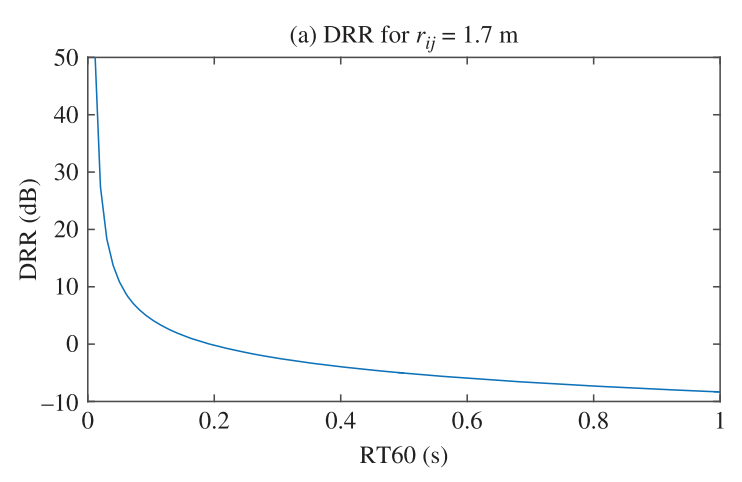
\includegraphics[width=\linewidth]{acoustics/drr_rt60.png}
    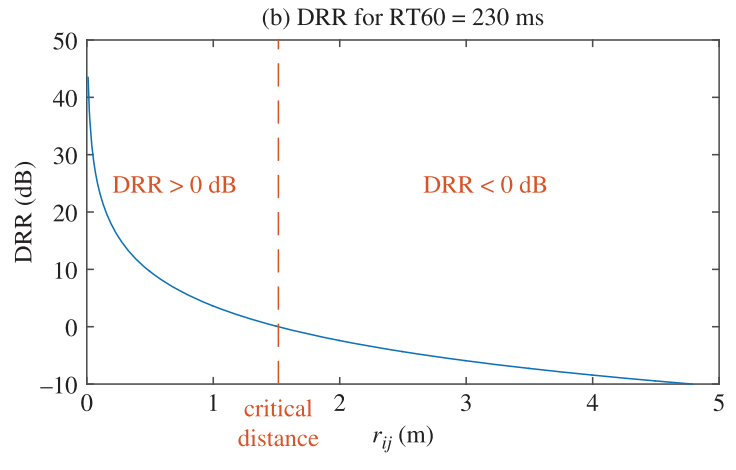
\includegraphics[width=\linewidth]{acoustics/ddr_dist.png}
    \captionof{figure}{%
        DRR as a function of the RT60 and the source distance rij based on Eyring’s formula (Gustafsson et al., 2003).
        These curves assume that there is no obstacle between the source and the microphone, so that the direct path exists.
        The room dimensions are the same as in Figure 3.1.
    }
    \label{fig:acoustics:drr}
}
% A proper analytical definition will be provided in the next chapter.
% % The $\DRR$ at the mth microphone in each microphone configuration was calculated using the method
% % \begin{equation}
% %     \DRR_\idxMic = 10 \log_{10}{\frac{
% %         \sum_{n=-\infty}^{\infty} \kparen{h^d_{ij}(n)}^2}%
% %         {\sum_{n=-\infty}^{\infty} \kparen{h^e_{ij(n)}}^2}}
% %         = 10 \log_{10}{\frac{
% %             \sum_{n=-\infty}^{\infty} \kparen{h^d_{ij}(n)}^2}%
% %             {\sum_{n=-\infty}^{\infty} \kparen{h^e_{ij}(n)}^2}}
% % \end{equation}
The distance beyond which the power of indirect sound becomes larger than that of direct sound is called the \textit{critical distance}.

These quantities represent an important parameter to assert the robustness of audio signal processing methods,
since they basically measure the validity of the free-field assumption.

% Similarly, one can define the \textit{direct-to-early ratio} ($\DER$), which is the power of direct sound divided by the remaining power in the first ??c samples (defined above),
% quantifies the modification of the power spectrum of the signal induced by early echoes.
%  It is low when the microphone and/or the source is close to an obstacle such as a table or a window, and higher otherwise.
%  The DRR and the direct-to-early ratio are not systematically reported when describing experiments in the literature,
%   yet they are as important as the RT60 to characterize multichannel mixtures

\chapter{Signal Processing and Audio Inverse Problem}\label{chap:processing}


\section{Signal Model}
This section is about the signal model


\subsection{Multichannel Mixing Process}

\subsection{Time-Frequency Analysis and Synthesis}

\subsection{Artificial Mixtures}

\subsection{Impulse Response Models}
\newthoughtpar{Acoustic and Room Impulse Response}

\newthoughtpar{Acoustic and Room Transfer Functions}

\newthoughtpar{Steering Vectors}

\newthoughtpar{Relative Transfer Functions}

\newthoughtpar{Full-Rank Covariance Models}

%%%%%%%%%%%%%%%%%%%%%%%%%%%%%%%%
\section{Audio Inverse Problems}
\newthoughtpar{Forward vs Inverse Problem}

\subsection{General Processing Scheme}
General Processing Pipeline

\subsection{Some Audio Inverse Problems}
\begin{enumerate}
    \item sound source separation and enhancements
    \item sound source localization
    \item microphones calibration
    \item channel estimation
    \item room geometry estimation
    \item acoustic echo estimation
\end{enumerate}
\newthoughtpar{Evaluation}

%%%%%%%%%%%%%%%%%%%%%%%%%%%%%%%%
\section{Taxonomy through dichotomies}
%% acoustics %%
\newthoughtpar{Single-Channel vs. Multichannel}
\newthoughtpar{Point vs. Diffuse Sources}
\newthoughtpar{Directonal vs. Onmidirectional Recordings}
\newthoughtpar{Diffuse vs. Measurements Noise}
%% processing %%
\newthoughtpar{Natural vs. Artificial Mixtures}
%% pipeline %%
\newthoughtpar{Problem vs. Model}
\newthoughtpar{Synthesis vs. Abstaction}
%% problems %%
\newthoughtpar{Separation vs. Enhancement}
%% models %%
\newthoughtpar{end2end vs. 2step}
end2end: from data to (feature to) target
\\2-step: (from data to features) + features to target

\newthoughtpar{Knowledge-based vs. Learning-based}
\begin{itemize}
    \item Bottom-up vs Top-down information processing
    \item Knowledge-based: specialized signal processing and mathematical algorithms informed by knowledge;
    \item Learning-based: machine learning usually trained in supervised fashion.
\end{itemize}

\newthoughtpar{Supervised vs. Unsupervised}
\newthoughtpar{Machine Learning vs. Deep Learning}
% \chapter{Evaluation and Datasets}\label{chap:evaluation}

\section{Metrics}
\subsection{Audio Signal Processing Metrics}

\section{Data and Dataset}
\subsection{Picnic of the Muses dB}
\subsection{dEchorate}





% %% II. Estimation
% \begin{fullwidth}
% \part{Acoustic Echo Retrieval}\label{pt:estimation}
% \end{fullwidth}
% \parttoc[n]
% \chapter{Acoustic Echo Estimation}\label{chap:estimation}

\section{Overview}
\begin{itemize}
    \item Acoustic Echo Retrieval definition
    \item Acoustic Echo Retrieval scope and placement in the signal processing pipeline
    \item Acoustic Echo Retrieval characteristic
\end{itemize}

\section{Echoes in the Time, Frequency and Cepstral domains}
\begin{itemize}
    \item Time domain processing
    \item Frequency domain processing
    \item Correlation processing
    \item Cepstral processing
\end{itemize}


\section{Related Works}
\subsection{Active vs. Passive echoes estimation}

\subsection{Knowledge-based vs. Data-driven}
\begin{itemize}
    \item Knowledge-driven (Physic-driven)
    \begin{itemize}
        \item Channel (RIR) estimation and Echoes pruning - Crooco and Dokmanic
        \item TDOA estimation (multipath) - Benesty
        \item Spikes Retrieval - Condat
    \end{itemize}
    \item Data-driven
    \begin{itemize}
        \item GLLiM
        \item Deep Leaning echo estimation
    \end{itemize}
\end{itemize}

\subsection{end-2-end vs 2-steps approaches}

AER\\
eRTF + AER

Pruning methods

\section{Related Works}

\subsection{AER as a RIR Estimation problem}
\todo{summarize Crocco's presentation}

TX signal: known vs. not known
\\TX signal not known: statistical methods and blind methods

\subsection{AER as a Spike Estimation problem}


\subsection{Virtually-supervised and Data Augmentation}


\section{Data and Metrics}
\subsection{Spike-based metrics}
% \chapter{Data-driven Acoustic Echo Retrieval \& \lantern}\label{chap:lantern}


% \chapter{Blaster: Knowledge-driven Acoustic Echo Retrieval}\label{chap:blaster}

% %Animals and humans have a remarkable ability to listen to the acoustic response of their environment.
% %Also known as \emph{echolocation} or \emph{bio-sonar}, it is used consciously and unconsciously to retrieve information about the environment and objects using sound waves.
% %Two (of the most) striking examples are bats and whales which use it as navigation and foraging mechanisms.

% %Striking introductive sentece
% In room acoustics and audio signal processing, the temporal structure of the room impulse response (RIR) plays a central role.
% % First echo is noise
% It is the result of multiple (indirect) sound propagation paths due to specular and diffuse reflections on the room's surfaces, leading to reverberation~\cite{Wang2011}.
% In such conditions, the perceived sound quality is often considered degraded and it is common to observe a detrimental decrease of performance as reverberation increases for applications such as speech recognition~\cite{Yoshoka2012} or music information retrieval~\cite{Barthet2010}.
% % or music virtual reality~\cite{DeMan2017}. %to observe a detrimental decrease of performances with reverberation. as well as music virtual reality~\cite{DeMan2017}.
% %\textcolor{red}{Add something about amazon echo, google assistant (analysis) and virtual reality (rendering/synthesis)}

% % Second echo is information
% On the other hand, RIRs contain very rich geometrical information about the acoustic scene.
% %which is independent from the source signal itself.
% %In contrast with well-consolidated methods,
% Recent \textit{echo-aware} works have shown that the knowledge of the timing of early reflections may boost performance in many audio signal processing applications, from dereverberation~\cite{Wu2006,Lin2008} to sound localization~\cite{Ribeiro2010,DiCarlo2019} and separation~\cite{Dokmanic2015a, Scheibler2017}.
% Moreover, it allows joint estimation of the receivers' positions~\cite{Salvati2016}, the reflective surfaces~\cite{Antonacci2012} and consequently the geometry of the room~\cite{Dokmanic2013, Crocco2017}.
% % or acoustic impedance of surfaces~\cite{Antonello2014, Bertin2016}.
% % beamforming \cite{Dockmanic2015},
% % such as for speech enhancement \cite{Wu2006}, source localization \cite{Ribeiro2010}, source separation \cite{Scheibler2017} and dereverberation \cite{Lin2009}
% % which are common pre-processing steps for many applications \cite{Gannot2017}

% Acoustic echo retrieval (AER) consists in estimating the properties of the early (strong) acoustic reflections only in multi-path environments~\cite{Tukuljac2018}, sometimes referred to as time delay estimation~\cite{Chen2006a}. To achieve this, several methods rely on a known source signal~\cite{park2017compressive,jensen2019method}.
% % Adding unknown adds a line :-(
% % yes, but it is really important
% % Got it. New mission: win space somewhere else in the paragraph?
% % no problem, I will pass throughthhtghththghth this
% % Seems legit
% In contrast, when multiple receivers attend an unknown single source, AER can be seen as an instance of Single Input Multiple Output (Blind) Channel Estimation (SIMO-BCE) problem.
% %or \textit{system identification}, \textit{i.e.} estimating the filters entailing an unknown input observed output of a system.
% %In a more challenging setting, when no prior information about the source signal are available, the problem is referred to as SIMO \textit{blind channel estimation} (SIMO-BCE) \cite{Lin2007}.
% A common approach for solving AER in the context of SIMO-BCE is to first blindly estimate a discrete version of the acoustic channels using the so-called cross-relation identity~\cite{Xu1995, Crocco2016}.
% The location of the echoes are then chosen among the strongest peaks with ad-hoc peak-picking techniques.
% %Such methods are generally \emph{on-grid} in the sense that the estimation relies on a fixed grid of points and \textit{a priori} chosen filter lengths.
% However, in practice, the true timings of echoes rarely match the sampling grid, thus leading to pathological issues called basis-mismatch in the field of compressed sensing.
% To circumvent this issue, the authors of~\cite{Tukuljac2018} proposed to leverage the framework of finite-rate-of-innovation sampling to make one step towards off-grid approaches.
% Despite promising results in the absence of noise and with synthetic data, the quality of the estimation highly relies on an initialization point.

% Of particular interest in this paper is the recently proposed framework of continuous dictionaries (CD)~\cite{Carlos2014}.
% By formulating an inverse problem as the recovery of a discrete measure over some parameter space, CD has allowed to overcome imaging device limitations in many applications such as super-resolution~\cite{Carlos2014} or PALM/STORM imaging~\cite{denoyelle2019}.
% In this work, we formulate the problem of stereo AER within the framework of continuous dictionaries.
% The resulting optimization problem is convex and thus not prone to spurious minimizers.
% The proposed method is coined \emph{Blind And Sparse Technique for Echo Retrieval} (\algoBraire) and requires no parameter tuning.
% The method is compared to state-of-the art on-grid approaches under various noise and reverberation levels using simulated data.
% While comparable or slightly worse recovery rates are observed for the task of recovering 7 echoes or more, better results are obtained for fewer echoes and the off-grid nature of the approach yields generally smaller estimation errors.

% \subsection{Signal and measurement model}

% Consider the common setup where a band-limited and square-integrable source signal $\contSource$ is emitted.
% Due to the geometry of the room, the latter signal is both reflected (several times) and attenuated before reaching a set of two microphones.
% The recorded signal at microphone $i\in\{1,2\}$ reads
% \begin{equation}
%     \label{eq:recordedSignal}
%     \contRecordedSignal_i = \contSource \ast \contFilter_i^\star + \contNoise_i
% \end{equation}
% where $\ast$ denotes the (continuous) convolution operator, $\contNoise_i$ models some additive noise in the measurement process and $\contFilter_i^\star$ denotes the room impulse response (RIR).
% In the remainder of this paper, the  superscript $\star$ refers to the ground truth.
% In AER, we are interested in RIRs that are streams of Diracs, \textit{i.e.},
% \begin{equation}
%     \label{eq:def_filter_star}
%     \contFilter_i^\star(t) = \sum_{r=0}^{R_i-1} c_{i,r} \delta(t - \tau_{i,r})
% \end{equation}
% where $R_i$ is the (unknown) number of echoes, $\kfamily{\tau_{i,r}}{r=0}^{R_i-1}$ models the echoes' delays, and $\kfamily{c_{i,r}}{r=0}^{R_i-1}$ are the corresponding non-negative attenuations.
% Note that $r=0$ defines the direct propagation path.
% %
% In the noiseless case, that is when $\contNoise_i=0$ for $i\in\{1,2\}$, we have the identity
% \begin{equation} \label{eq:cross-relation}
%     \contRecordedSignal_1 \ast \contFilter_2^\star = \contRecordedSignal_2 \ast \contFilter_1^\star
% \end{equation}
% by commutativity of the convolution operator.
% This result is dubbed cross-relation identity in the channel identification literature \cite{Xu1995}.
% Hence, one can expect to recover the two filters by solving an optimization problem involving~\eqref{eq:cross-relation}.
% %the difference between the two terms in~\eqref{eq:cross-relation}.

% However, in practice, only sampled versions of the two recorded signals are available.
% More precisely, we consider a  measurement model where the incoming signal undergoes a (ideal) low-pass filter $\idealLowPassFilter$ with frequency support $\kintervcc{\sfrac{-\SamplingFreq}{2}}{\sfrac{\SamplingFreq}{2}}$ before being regularly sampled at the rate  $\SamplingFreq$.
% We denote $\disRecordedSignal_1,\disRecordedSignal_2\in\kR^{2N}$ the two vectors of $2N$ (consecutive) samples and $i\in\{1, 2\}$ by
% \begin{equation}
%     \label{eq:measurement-process}
%     \disRecordedSignal_i[n] =
%     \kparen{\idealLowPassFilter \ast \contRecordedSignal}\kparen{\frac{n}{\SamplingFreq}}
%     \qquad
%     \forall n \in\{0, \dots, 2N-1\}
%     .
% \end{equation}
% %Let $\disRecordedSignal_1,\disRecordedSignal_2\in\kR^N$ denote the two vectors of $N$ consecutive samples that are such that $\disRecordedSignal_i[\ell] = \contRecordedSignal_i(\sfrac{\ell}{F_s})$ for $\ell\in\{1...N\}$, $i\in\{1, 2\}$ and  where $F_s$ is the sampling frequency.



% %We denote $\disRecordedSignal\in\kR^N$ the $N$ consecutive samples, \textit{i.e.}, such that $\disRecordedSignal[\ell] = \contRecordedSignal(\sfrac{\ell}{F_s})$ where $F_s$ is the sampling frequency.
% % These $N$ consecutive samples will be denoted  $\disRecordedSignal\in\kR^N$ and satifies $\disRecordedSignal[\ell] = \contRecordedSignal(\sfrac{\ell}{F_s})$ $\forall\ell\in\{1...N\}$ where $F_s$ is the sampling frequency.

% %the signals are notaccessible.  They are measured by sensors and discretized to be stored in a computer’s memory.


% \subsection{Existing works}
% Starting from the identity \eqref{eq:cross-relation}, the common SIMO BCE cross-relation framework aims to compute $\contFilter_1, \contFilter_2$ solving the following LASSO-type problem in the discrete-time domain:
% \begin{multline}
%     \label{eq:xrel_toepl}
%     %\begin{split}
%     \disFilterHat_1, \disFilterHat_2
%     =
%     \kargmin_{\disFilter_1, \disFilter_2}
%     \;
%     \kvvbar{
%         \calT(\disRecordedSignal_1) \disFilter_2
%         -
%         \calT(\disRecordedSignal_2) \disFilter_1
%     }_2^2
%     +
%     \lambda
%     \kvvbar{
%         \disFilter
%     }_1
%     \\
%     %\quad
%     \text{s.t.} \quad \disFilter[0] = 1
%     \qquad
%     %\qquad
%     %\end{split}
% \end{multline}
% where $\disRecordedSignal_i$ and $\disFilter_i$ are the discrete, sampled version of $\contRecordedSignal_i, \contFilter_i$ respectively and $\disFilter = [\disFilter_1^\intercal, \disFilter_2^\intercal]$.
% $\calT(\disRecordedSignal_i)$ is the $(2N+L-1) \times L$ Toeplitz matrix\footnote{The first row and column of $\calT(\disRecordedSignal_i)$ are respectively $[\disRecordedSignal_i[2N-n], 0,\dotsc,0]$ and $[\disRecordedSignal_i[2N-n], \disRecordedSignal_i[2N-n+1],\dotsc,\disRecordedSignal_i[n], 0,\dotsc, 0]^\intercal$.} associated to convolution where $2N$ and $L$ respectively denote  microphone and filter signal length.
% The constraint $\disFilter[0]=1$ is called an anchor constraint.

% The accuracy of estimated RIRs has been subsequently improved using a priori knowledge of the filters: in particular, the authors of~\cite{Lin2007} have proposed to use sparsity penalty and non-negativity constraints to increase robustness to noise as well as Bayesian-learning methods to automatically infer the value of $\lambda$ in~\cite{Lin2008}.
% Even if sparsity and non-negativity could be seen as a strong assumption, works in speech enhancement~\cite{Ribeiro2010,Dokmanic2015a} and room geometry~\cite{Antonacci2012,Crocco2017} estimation have proven the effectiveness of this approach.
% On a similar scheme, in~\cite{Kowalczyk2013},~\eqref{eq:xrel_toepl} is solved using an adaptive time-frequency-domain approach while~\cite{Aissa-El-Bey2008} proposes to use the $\ell_p$-norm instead of the $\ell_1$-norm.
% A successful approach has been presented recently by Crocco \textit{et al.} in \cite{Crocco2016}, where the anchor constraint is replaced by an \textit{iterative weighted} $\ell_1$ equality constraint.
% %, \corrCE{ \textit{i.e.}, such that $\langle{\bfh^{(t-1)},\bfh^{(t)}}\rangle=1$ at each iteration $t$ where $\bfh^{(0)}$ is the solution of~\eqref{eq:xrel_toepl}.}

% %$\bfp^{(z)\intercal}\disFilter = 1$, for the iteration $(z)$\footnote{Note that when $\bfp^{(z)} = 1$, the constraint returns to the $\ell_1$ penalty.}. In particular, the method is initialized using the solution of \cite{Lin2007} and iterated enforcing sparsity using the solution of the previous problem, that is $\bfp^{(z)} = \disFilterHat^{(z-1)}$.

% %{\color{blue}
% %A Diego : ho scritto le seguenti frasi prima.
% %Non si adattano piu alla mia sezione.
% %Forse puoi farne uso:
% %\begin{itemize}
% %    \item Therefore, one may reasonably consider recovering $\contFilter_1$ and $\contFilter_2$ by solving an optimization problem involving the cross-relation identity.

% %    \item However, one would have to pay attention not selecting trivial solution such as $(\contFilterHat_1, \contFilterHat_2)=(0,0)$.

% %    \item To circumvent this issue, additional explicit constraints on the solution have been considered such as imposing a minimal energy~\cite{Kowalczyk2013} or weighted linear constraints~\cite{Crocco2016}.

% %    \item In this paper, we restrict our attention to the so-called \emph{anchor constrained} $\contFilter_1(0)=1$ which can be interpreted as choosing the origin of time.
% %\end{itemize}
% %}



% %\begin{itemize}
%     %\item Start from noiseless signal model

%     %\item Consider a setup where a \textcolor{blue}{band-limited?} and square-integrable source signal $\contSource$ is emitted.
%     %Due to the geometry of the room, the source $\contSource$ is  both reflected several times and attenuated before reaching a set of two microphones.

%     %\item The recorded signal at microphone $i\in\{1,2\}$ writes
%     %\begin{equation}
%     %    \label{eq:recordedSignal}
%     %    \contRecordedSignal_i = \contSource \ast \contFilter_i^\star + n_i
%     %\end{equation}
%     %where $\ast$ denotes the (continuous) convolution operator, $n_i=0$ models some additive noise in the measurements and $\contFilter_i$ denotes the Acoustic Impulse Response (AIR).

%     %\item Following the \textcolor{blue}{XXX model}, the AIR can be modeled using a stream of Dirac, that is
%     %\begin{equation}
%     %    \label{eq:def_filter_star}
%     %    \contFilter_i^\star(t) = \sum_{k=1}^{K_i} c_{i,k} \delta(t - \tau_{i,k})
%     %\end{equation}
%     %where $K_i$ is the (unknown) number of echoes, $\kfamily{\tau_{i,k}}{k=1}^{K_i}$ models the echo delay, and $\kfamily{c_{i,k}}{k=1}^{K_i}$ are the corresponding to attenuations.


%     %\item In the noiseless case, that is when $n_i=0$ for $i=1,2$, it has been noticed that $\contRecordedSignal_1 \ast \contFilter_2 = \contRecordedSignal_2 \ast \contFilter_1$ or, equivalently in the Fourier domain
%     %\begin{equation}
%     %    \label{eq:cross-relation-identity}
%     %    \calF[\contRecordedSignal_1] \cdot \calF[\contFilter_2^\star]
%     %    =
%     %    \calF[\contRecordedSignal_2] \cdot \calF[\contFilter_1^\star]
%     %\end{equation}
%     %by associativity of the convolution operator and where $\calF$ is such that\footnote{Note that we use the same notation when referring to the Fourier transform of a function and a distribution.}
%     %\begin{equation}
%     %    \kforall[f\in\kR]\quad \calF[y] =
%     %    \int_{-\infty}^{+\infty} y(t)\cste^{-\csti2\pi f t}\,\mathrm{d}t
% %        \kfuncdef{\calF}{L^2(\kR)}{L^2(\kR) \textcolor{blue}{\quad \text{a definir}}}[x][
%  %           \displaystyle
%  %           \kfamily{
%  %           f\mapsto \int_{-\infty}^{+\infty} x(t)\cste^{-\csti2\pi\ell t}\,\mathrm{d}t
%  %           }{\ell=-\infty}^{+\infty}
%  %           .
%  %       ]
%     %\end{equation}
%     %for all signal or filter $y$.
%     %The relation~\eqref{eq:cross-relation-identity} is dubbed \emph{cross-relation} identity in the acoustic literature~\textcolor{blue}{\cite[Correct?]{Tong1994}}, and may be considered as more convenient since it only involves matrix multiplications.
% %    \begin{equation}
% %        \label{eq:cross-relation-identity}
% %        \contRecordedSignal_1 \ast \contFilter_2 = \contRecordedSignal_2 \ast \contFilter_1
% %    \end{equation}




%     %\item Therefore, on may reasonably consider recovering $\contFilter_1$ and $\contFilter_2$ by solving an optimization problem involving the cross-relation identity.
%     %However, one would have to pay attention not selecting trivial solution such as $(\contFilterHat_1, \contFilterHat_2)=(0,0)$.
%     %To circumvent this issue, additional constraints on the solution has been considered, see for instance~\textcolor{blue}{?}.
%     %In this paper, we restrict our attention to the so-called \emph{anchor constrained} $\contFilter_1(0)=1$ which can be interpreted as choosing the origin of time.
%     %Hence one can expect recover $\contFilter_1^\star$ and $\contFilter_2^\star$ by solving
%     %\begin{equation}
%     %    \label{eq:ideal-infinite-problem}
%     %    \begin{split}
%     %    \contFilterHat_1, \contFilterHat_2
%     %    =
%     %    \kargmin_{\contFilter_1, \contFilter_2\in\textcolor{blue}{todo}}
%     %    \;
%     %    \kvvbar{
%     %        \calF[\contRecordedSignal_1] \cdot \calF[\contFilter_2]
%     %        -
%     %        \calF[\contRecordedSignal_2] \cdot \calF[\contFilter_1]
%     %    }_2^2
%     %    \\
%     %    \quad \text{s.t.} \quad \contFilter_1(0) = 1
%     %    . \qquad\qquad\qquad
%     %    \end{split}
%     %\end{equation}
%     %Indeed, one immediately sees that the couple $(\contFilter_1^\star,\contFilter_2^\star)$ is a minimizer of~\eqref{eq:ideal-infinite-problem}.

%     %\item Unfortunately, due to the measurement process, one has only access to a sampled version $\disRecordedSignal_i\in\kR^N$ of the recorded signal, or equivalently, the lower end of the spectrum of $\disRecordedSignal_i$.
%     %More precisely, the information we have about $\disRecordedSignal_i$ takes the form of the lowest $2N+1$ coefficients of the Fourier series given by
%     %\begin{equation}
%     %    \label{eq:dft-Xi}
%     %    X_i[f] = \sum_{n=0}^{N-1}
%     %    \contRecordedSignal_i(nT_e)
%     %    \cste^{-\csti2\pi fnT_e}
%     %\end{equation}
%     %where $X_i$ denotes the Discrete Fourier transform of $\contRecordedSignal_i$, $T_e$ is the sampling period and $f$ belongs to the \emph{finite} set of \emph{regularly-spaced} frequency $\kset{\frac{n}{T_e}}{n=0\dots N-1}$.



%     %\item The cross-relation identity~\eqref{eq:cross-relation-identity} remains nevertheless true for the $N$ available Fourier coefficients.\footnote{To be more precise, $2N-1$ coefficients are available. However, since the recorded signals $\contRecordedSignal_i$ are real, $N$ Fourier coefficients are sufficient to describe the Discrete Fourier Transform.}
%     %Whereas one could replace the Fourier transforms in~\eqref{eq:ideal-infinite-problem} by their Fourier series counterpart,
%     %the problem becomes ill posed since infinitely many solutions are available.



%     %\item \textcolor{blue}{What do we do with the door in time domain? in Mulan they say that $X_i$ is a good approximation of the FT as $N$ tends to infinity right?
%     %$\rightarrow$ sinus cardinal, has to be cancelled? could be done since the the source signal is assumed band limited with a correct sampling frequency}
% %\end{itemize}


% %!TEX root = ../icassp2020braire.tex

% %\textcolor{red}{Todo:
% %\begin{itemize}
%     %\item Find the correct number of Fourier coefficient
%     %
%     %\item Renormalized atom?
%     %\item Define what is a filter - function in the first section and measure in the second?
%     %Or directly talk about radon measure since the beginning?
%     %
%     %\item Introduce the CTDF of $\contFilter$ in the equation (instead of the Fourier transform)
%     %
%     %\item Introduce the dictionary before~\eqref{eq:TV-BP}.
% %\end{itemize}
% %}

% %\textcolor{blue}{What do we do with the door in time domain? in Mulan they say that $X_i$ is a good approximation of the FT as $N$ tends to infinity right?
% %$\rightarrow$ sinus cardinal, has to be cancelled? could be done since the the source signal is assumed band limited with a correct sampling frequency}




% %\remCE{TODO intro after related work is written}
% %All the methods presented above rely on a discrete formulation of the Cross-Relation identity~\eqref{eq:cross-relation}, thus relying on a T\oe{}plitz formulation of the convolution.
% %\remCE{Add drawbacks, such as on-the-grid}
% %In this work, we propose to circumvent this issue by casting the estimation problem in the \emph{continuous dictionaries} framework.


% \subsection{Cross-relation in the Fourier domain}

% \newcommand{\paramVec}[1]{\Delta_{#1}}

% We first remark that the cross-relation identity~\eqref{eq:cross-relation} ensures that the relation
% $   \idealLowPassFilter
%     \ast \contRecordedSignal_1
%     \ast  \contFilter_2^\star
%     =
%     \idealLowPassFilter
%     \ast \contRecordedSignal_2
%     \ast  \contFilter_1^\star
% $
% %by associativity of the convolution operator,
% %or equivalently
% holds, hence
% \begin{equation}
%     \label{eq:cross-relation-identity-fourier}
%     \fourierTrans(\idealLowPassFilter\ast\contRecordedSignal_1) \cdot \fourierTrans \contFilter_2^\star
%     =
%     \fourierTrans(\idealLowPassFilter\ast\contRecordedSignal_2) \cdot \fourierTrans \contFilter_1^\star
% \end{equation}
% where $\fourierTrans$ denotes the Fourier transform (FT)
% % and is such that %\footnote{}
%  \begin{equation}
%      \kforall[f \in\kR]\quad \fourierTrans y(f) =
%      \int_{-\infty}^{+\infty} y(t)\cste^{-\csti 2 \pi f t}\,\mathrm{d}t
%  \end{equation}
%  for any signal or filter $y$ (note that we use the same notation when referring to the Fourier transform of a function and a distribution).
% %We thus propose to use~\eqref{eq:cross-relation-identity-fourier} in a penalized least-square problem akin to~\eqref{eq:xrel_toepl}.
% %Such a formulation in the Fourier domain may even be considered as more convenient since the convolution operator is no longer involved.

% %\corrCE{In particular,~\eqref{eq:cross-relation-identity-fourier} remains true when evaluated at the set of regularly-spaced frequencies $0,1/\SamplingFreq\dots(N-1)/F_s$.}
% While the FT of $\contFilter_i^\star$ can be expressed in closed-form (see~\eqref{eq:closed-form-TF-dirac-N} below), the FT of $\idealLowPassFilter\ast\contRecordedSignal_i$ is not available due to the measurement process.
% To circumvent this issue, we use the %propose the following
% approximation
% %to approximate it by the discrete Fourier Transform of $\bfx$
% \begin{equation}
%     \label{eq:approx-TF}
%     \fourierTrans(\idealLowPassFilter\ast\contRecordedSignal_i)
%     %(\tfrac{f}{F_s})
%     (\tfrac{k}{2N}F_s)
%     \simeq
%     X_i[k]
% \end{equation}
% %for all $f\in\{0\dots N-1\}$
% % \corrRG{for all integers $f \in \{-N/2+1, \ldots, N/2\}$,}
% for all integers  $k \in \{0, \ldots, N\}$,
% where
% \begin{equation}
%     \label{eq:dft-Xi}
%     \RecordedSignalDFT_i[k] = \sum_{n=0}^{2N-1}
%     \bfx_i[n]
%     \cste^{-\csti2\pi \tfrac{kn}{2N}} %/\SamplingFreq}
% \end{equation}
% is the discrete Fourier transform of the real vector $\bfx_i$ for positive frequencies only.
% The FT of $\contFilter_1^\star,\contFilter_2^\star$ (see~\eqref{eq:def_filter_star}) can be expressed in closed-form.
% Denoting $\paramVec{\tau}$ the following parametric vector of complex exponential
% \begin{equation}
%     \label{eq:closed-form-TF-dirac-N}
%     \paramVec{\tau} \triangleq
%     %\corrRG{\triangleq}
%     \left(\cste^{-\csti2\pi\tfrac{k}{2N}F_s \tau}\right)_{0 \leq k \leq N}
%     %  \ktranspose{
%     %  \begin{pmatrix}
%     %      \cste^{-\csti2\pi\tfrac{0}{T_e}\tau} &
%     %      \hdots &
%     %      \cste^{-\csti2\pi\tfrac{N-1}{T_e}\tau}
%     %  \end{pmatrix}
%     % }
%     \in\kC^{N+1}
%     ,
% \end{equation}
% equation~\eqref{eq:cross-relation-identity-fourier} evaluated at $f = \frac{k}{2N}F_s$ where $k \in \{0,\ldots, N\}$
% reads

% \begin{equation}
%     \label{eq:cross-relation-approx}
%     \sum_{r=0}^{R_2-1}\bfX_1 \odot \paramVec{\tau_{2,r}}
%     =
%     \sum_{r=0}^{R_1-1}\bfX_2 \odot \paramVec{\tau_{1,r}}
% \end{equation}
% where $\odot$ denotes the component-wise Hadamard product.








% \subsection{Echo localization with continuous dictionaries}




% By interpreting the FT of a Dirac as a parametric atom, we propose to cast the problem of RIR estimation into the framework of continuous dictionaries.
% To that aim, let us define the so-called \emph{parameter set}
% \begin{equation}
%     \label{eq:parameter-set}
%     \Theta \triangleq \kintervcc{0}{T} \times \kbrace{1, 2}
% \end{equation}
% where $T$ is the length (in time) of the filter.
% %We let the reader check that $\Theta$ is a compact metrizable set.
% Then, the two desired filters  $\contFilter_1^\star,\contFilter_2^\star$ given  by~\eqref{eq:def_filter_star} can be uniquely\footnote{Uniqueness is ensured as soon as we impose $c_{i,r}>0$ $\forall i,r$.} represented by the following discrete measure over $\Theta$
% \begin{equation}
%     \label{eq:representation_filter_measure}
%     \mu^\star = \sum_{i=1}^{2} \sum_{r=0}^{R_{i}-1} c_{i,r} \delta_{(\tau_{i,r}, i)}.
% \end{equation}
% The rationale behind~\eqref{eq:parameter-set}  and~\eqref{eq:representation_filter_measure} is as follows.
% A couple of filters is now represented by a single stream of Diracs, where we have considered an augmented variable $i$ indicating to which filter the spike belongs.
% For instance, a Dirac at $(\tau, 1)$ indicates that the first filter contains a Dirac at $\tau$.
% %\remCE{rather talk about TDOA?}

% The set $\posDisRadonMeasure$ of all unsigned and discrete Radon measures over $\Theta$ (\textit{i.e.}, the set of all couples of  filters) is equipped with the total-variation norm (TV-norm) $\normTV{\mu}$.
% % defined for any measure $\mu$ as
% % \begin{equation}
% %     \normTV{\mu} \triangleq
% %     \sup_{P}\; \sum_{E\in P} \kvbar{
% %         \mu(E)
% %     }
% % \end{equation}
% % where the supremum is taken over all partitions $P$ of $\Theta$ into a finite number of disjoint measurable subsets.\footnote{See~\cite{Rudin1987} for a rigorous construction of measures set and the TV-norm.}
% See~\cite{Rudin1987} for a rigorous construction of measures set and the TV-norm.
% % In this work, we restrict our attention to the set $\posDisRadonMeasure$ of unsigned and discrete Radon measures \corrCE{-- \textit{i.e.}, linear combinations of Dirac with positive coefficients --} over $\Theta$ with \emph{finite} TV-norm.
% We now define the \emph{linear} observation operator $\kfuncdef{\opObs}{\posDisRadonMeasure}{\kC^{N+1}}$, which is such that
% \begin{equation}
%     \opObs\delta_{(\tau, i)}
%     =
%     \begin{cases}
%         - \RecordedSignalDFT_1 \odot \paramVec{\tau}  &\text{ if } i=1 \\
%         + \RecordedSignalDFT_2 \odot \paramVec{\tau}  &\text{ if } i=2.
%     \end{cases}
% \end{equation}
% $\forall(\tau,i)\in\Theta$ where the two complex vectors $\RecordedSignalDFT_1, \RecordedSignalDFT_2$ have been defined in~\eqref{eq:dft-Xi} and $\calF_N\delta_\tau$ in~\eqref{eq:closed-form-TF-dirac-N}.

% %and the minimization is carried over the space of finite Radon measures.
% Then, by linearity of the observation operator $\opObs$, the relation~\eqref{eq:cross-relation-approx} can be rewritten as %evaluated at the $N$ considered frequencies \corrCE{can be rewritten as}
% \begin{equation}
%     \label{eq:cross-relation-measure}
%     \opObs\mu^\star = {\bf0}_{N+1}
%     .
% \end{equation}
% Before continuing our exposition, we note that the anchor constraint can be written in a more convenient way.
% Indeed, the constraint $\mu(\{(0, 1)\})=1$ ensures the existence of a Dirac at $0$ in the filter 1.
% Then, the targeted filter reads
% \begin{equation}
%     \mu^\star = \delta_{(0, 1)} + \widetilde{\mu}^\star
% \end{equation}
% where $\widetilde{\mu}^\star$ is a (finite) discrete measure verifying  $\widetilde{\mu}^\star\kparen{\{(0, 1)\}} = 0$.
% Denoting $\bfy\triangleq-\opObs\delta_{(0, 1)}\in\kC^{N+1}$, the relation~\eqref{eq:cross-relation-measure} becomes
% \begin{equation}
%     \label{eq:cross-relation-measure-and-obs}
%     \opObs\widetilde{\mu}^\star = \bfy
%     .
% \end{equation}
% For the sake of clarity, we use these conventions hereafter and omit the tilde.
% Now, following~\cite{Castro2012aa,Carlos2014}, one can expect to recover the desired filter $\mu^\star$ by solving
% \begin{equation}
%     \stepcounter{equation}
%     \tag{\theequation-$\calP^0{\text{\texttt{TV}}}$}
%     \label{eq:TV-BP}
%     %\begin{split}
%     \widehat{\mu}
%     =
%     \kargmin_{\posDisRadonMeasure}
%     \;
%     \normTV{
%         \mu
%     }
%     %\\
%     %
%     \quad
%     \text{s.t.}
%     \quad
%     \begin{cases}
%         \opObs\mu
%         = \bfy \\
%         \mu(\{(0, 1)\}) = 0.
%     \end{cases}
%     %\end{split}
% \end{equation}
% Note that~\eqref{eq:TV-BP} has to be interpreted as a natural extension of the well-known \emph{basis pursuit} problem to the continuous setting.
% Indeed, for \emph{any} finite discrete measure $\mu = \sum_{r=0}^{R-1} c_r\delta_{(\tau_r, i_r)}$, the TV-norm of $\mu$ returns to the $\ell_1$-norm of the coefficients, \textit{i.e.}, $\kvvbar{\mu}_{TV} = \sum_{r=0}^{R-1} \kvbar{c_r}$.
% %\corrCE{To model the both}

% Finally,~\eqref{eq:cross-relation-measure-and-obs} can be exploited to take into account noise during the measurement process (\textit{i.e.},  $n_i\neq0$ in~\eqref{eq:recordedSignal}), as well as approximation errors  (see~\eqref{eq:approx-TF}-\eqref{eq:cross-relation-approx}).
% In that case, the first equality constraint in~\eqref{eq:TV-BP} is relaxed, leading to the so-called Beurling-LASSO (BLASSO) problem
% \begin{equation}
%     \stepcounter{equation}
%     \tag{\theequation-$\calP^\lambda_{\text{\texttt{TV}}}$}
%     \label{eq:TV-BLASSO}
%     \begin{split}
%     \widehat{\mu}
%     =
%     \kargmin_{\mu \in\posDisRadonMeasure}
%     \;
%     \tfrac{1}{2} \kvvbar{
%         \bfy - \opObs\mu
%     }_2^2
%     +
%     \lambda\normTV{
%         \mu
%     }
%     \\
%     %
%     \quad
%     \text{s.t.}
%     \quad
%     \mu(\{(0, 1)\}) = 0
%     .
%     \end{split}
% \end{equation}
% We emphasize that although continuous Radon measures may potentially be admissible, the minimizers of~\eqref{eq:TV-BLASSO} are \emph{guaranteed} to be streams of Dirac\textit{s}~\cite[Theorem~4.2]{bredies2018sparsity}.
% In addition, although problem~\eqref{eq:TV-BLASSO} seems to depend on some regularization parameter $\lambda$, we describe in Section~\ref{sec:xp} a procedure to automatically tune it to recover a desired number of spikes.

% Finally, note that problem~\eqref{eq:TV-BLASSO} is convex with linear constraints.
% %Hence, it can be solved with standard convex optimization methods.
% In this work, we particularize the sliding Frank-Wolfe algorithm proposed in~\cite{denoyelle2019} to solve~\eqref{eq:TV-BLASSO}.
% Detailed descriptions of the steps of the algorithm are given in \ifthenelse{\boolean{compmat}}{\Cref{sec:SFW}.}{\cite[App.~A]{DiCarlo2020SupMat}.}
% %the supplementary material\footnote{\url{https://gitlab.inria.fr/panama-team/blaster/blob/master/algorithm.pdf}.}.


% \begin{figure*}[ht]
%     \centering
%     %\begin{minipage}{0.49\textwidth}
%         \centering
%         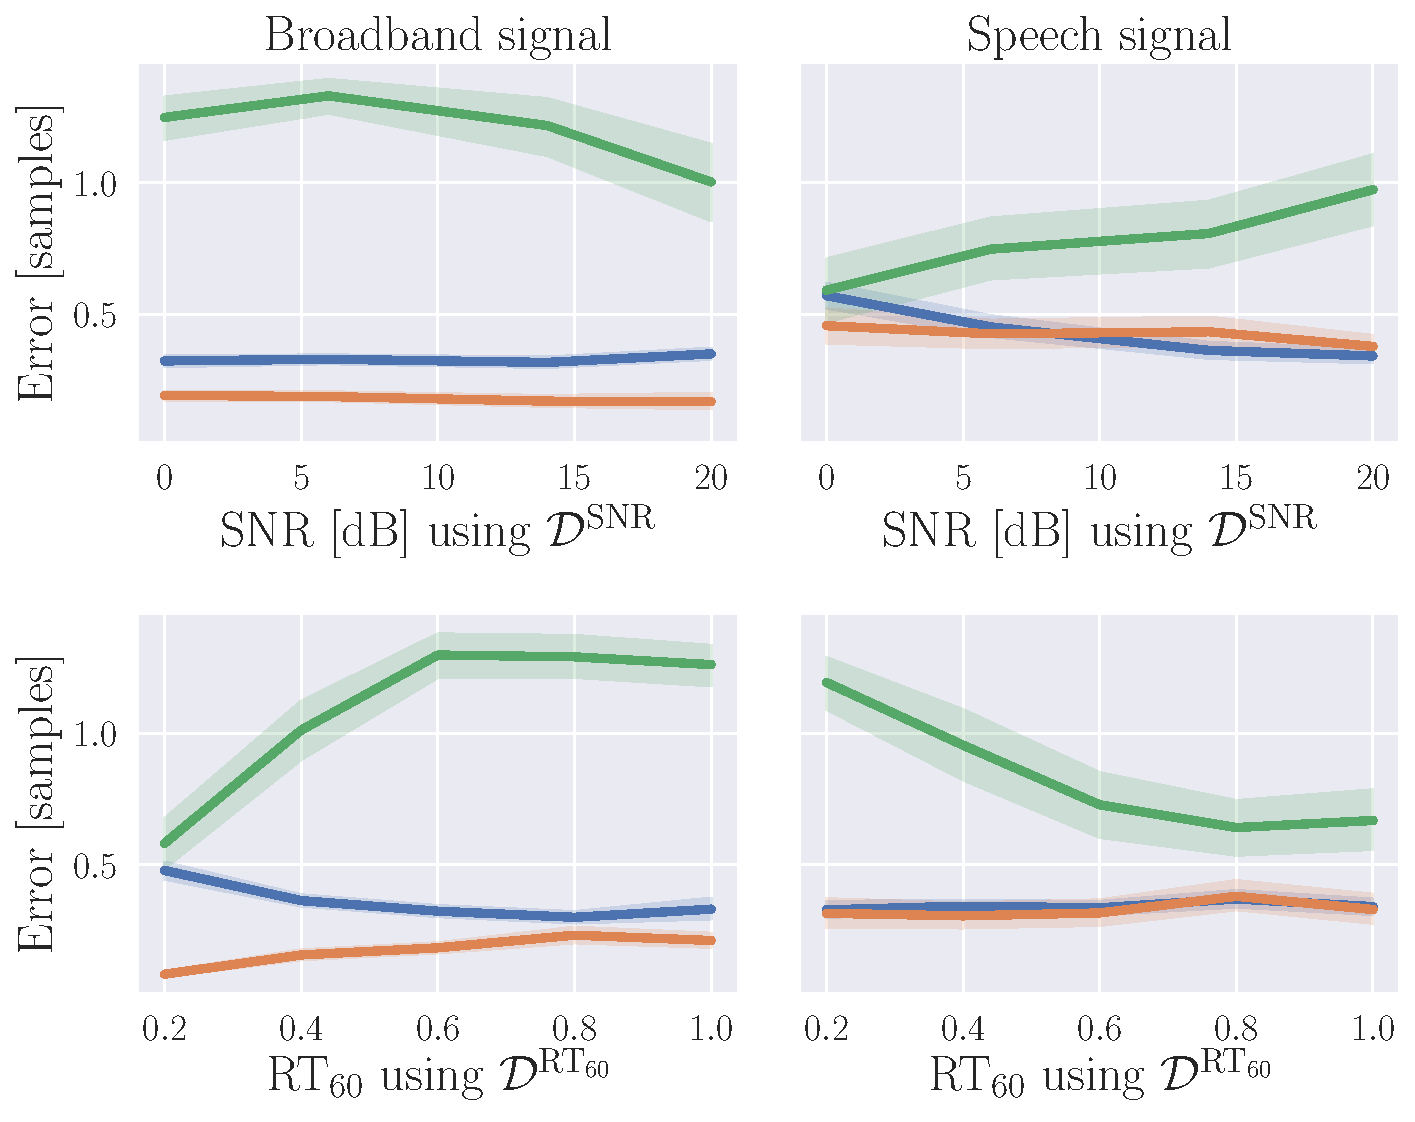
\includegraphics[width=.49\textwidth]{figures/e_k-7_thr-2_bns_crocco_blaster.pdf}
%         %\caption{\label{fig:error} Error}
%     %\end{minipage}\hfill
%     %\begin{minipage}{0.49\textwidth}
%     %    \centering
%         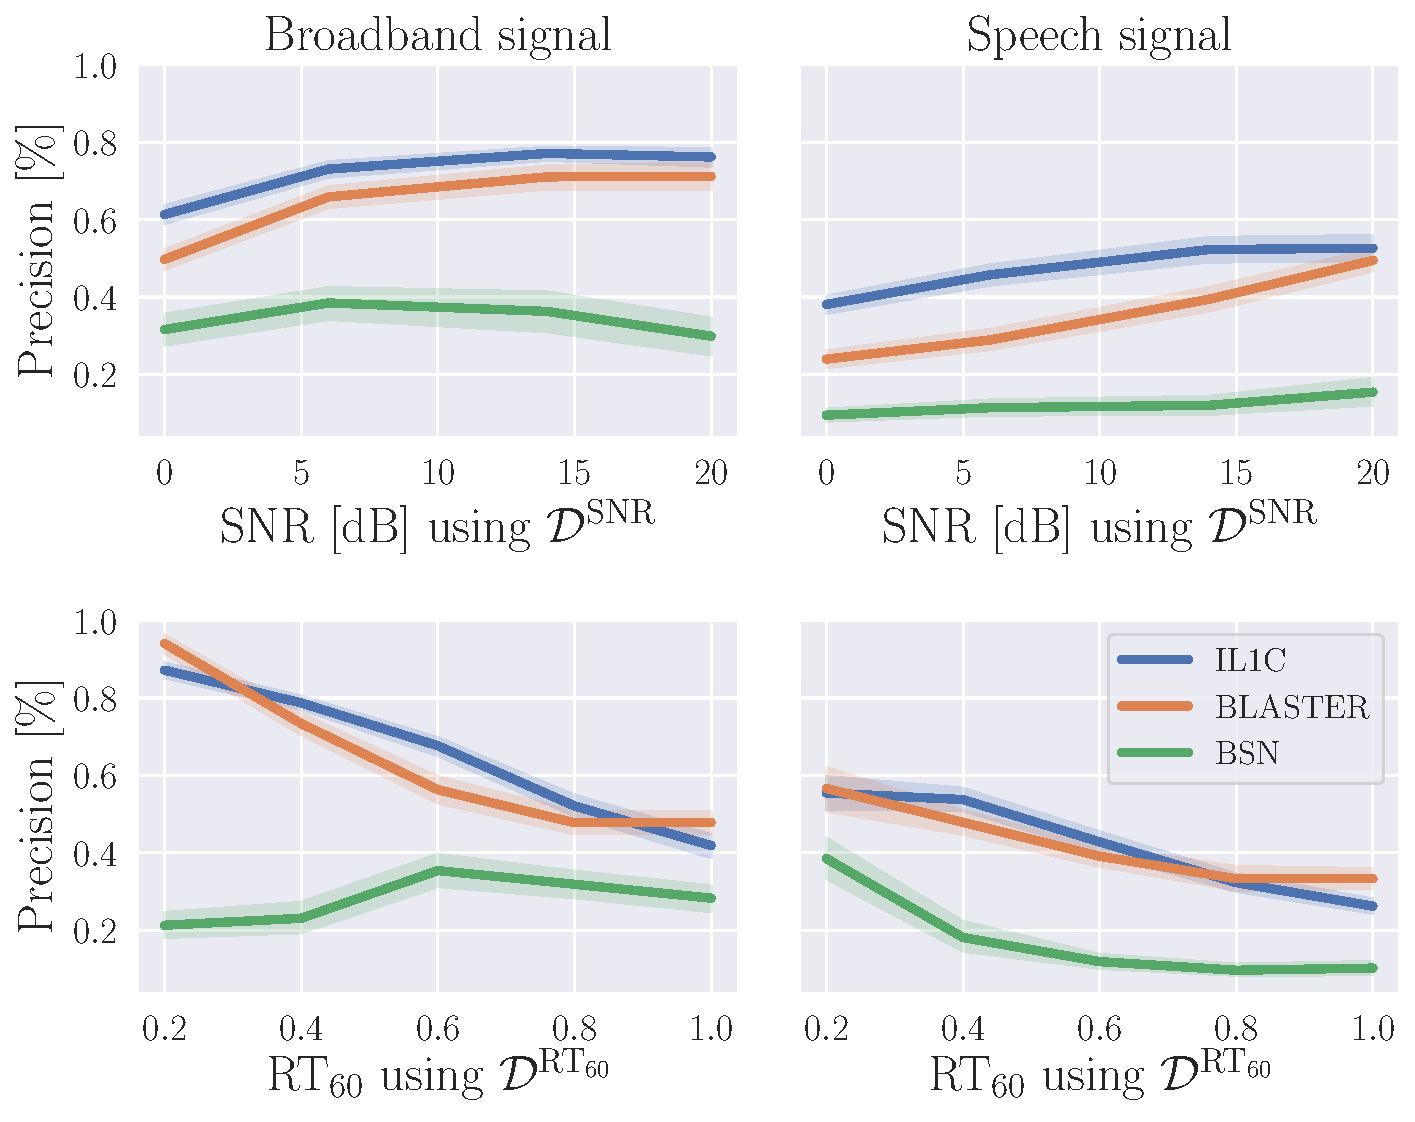
\includegraphics[width=.49\textwidth]{figures/p_k-7_thr-2_bns_crocco_blaster.pdf}
%         %\caption{\label{fig:precision} Precision}
%     %\end{minipage}

%     \vspace*{2pt}
%     \begin{center}
%     \caption{
%         \label{fig:error_precision_snr_rt}
%     Line plot with error bands for error (left) and precision (right) versus SNR level (top) and \RT{} level (bottom) using broadband and speech signals for the task of recovering $R=7$ echoes. A threshold of $\tau_{\textrm{max}}=2$ samples is used to compute the precision.
%     %The performances are computed with respect to the corresponding datasets \dsetSNR{} and \dsetRT{} as explained Section~\ref{sec:xp}.
%     }
%     \end{center}
% \vspace{-3mm}
% \end{figure*}



% The proposed method (\algoBraire) is compared against the non-negative $\ell_1$-norm method (\algoBsn) of~\cite{Lin2007} and the iterative $\ell_1$-norm approach (\algoCrocco) described in~\cite{Crocco2016}.
% The problem is formulated as estimating the time location of the first $R=7$ strongest components of the RIRs for 2 microphones listening to a single sound source in a shoebox room. It corresponds to the challenging task of estimating
% %all the
% first-order early reflections.
% The robustness of the methods is tested against different level of noise (SNR) and reverberation time (\RT{}).

% We propose to compute a \textit{path of solutions} to automatically estimate the regularization parameter $\lambda$  in~\eqref{eq:TV-BLASSO}.
% More precisely, let $\lambda_{\max}$ be the smallest value of $\lambda$ such that the null measure is the solution to~\eqref{eq:TV-BLASSO}.
% It can be shown that $\lambda_{\max}$ is upper bounded by $\max_{\theta\in\Theta} \kvbar{\bfy^\intercal\opObs\delta_\theta}$.
% Starting from $\ell=1$ and the empty filter, we consider a sequential implementation where the solution of~\eqref{eq:TV-BLASSO} is computed for $\lambda_\ell= 10^{-0.05\ell}\lambda_{\max}$ until the desired number of spikes is found in each channel when incrementing $\ell$.
% For each $\lambda_\ell$, we search for a solution of~\eqref{eq:TV-BLASSO} with the solution obtained for $\lambda_{\ell-1}$ as a warm start.

% The quality of the AER estimation is assessed in terms of precision\footnote{Since only $K$ time locations are considered in both the ground truth and the estimation, precision and recall are equal.} in percentage as in the literature of onset detection~\cite{Bock2012} and the root-mean-square-error (RMSE) in samples.
% Both metrics evaluate only the \textit{matched} peaks, where a \textit{match} is defined as being within a small window $\thr$ of a reference delay. These two metrics are similar to the ones used in~\cite{Crocco2015}.

% For this purpose we created three synthetic datasets of $1000$ observations each:
% %As summarized in Table~\ref{tab:datasets},
% \dsetValid{} is used for tuning the hyperparameter $\lambda$ and the peak-picking parameters for \algoCrocco{} and \algoBsn{} using \RT{} and SNR randomly drawn from $\mathcal{U}[0, 1]$ (sec) and $\mathcal{U}[0, 20]$ (dB) respectively; \dsetSNR{} features SNR value uniformly sampled in $[0, 6, 14, 20, \infty]$ while the \RT{} is kept fixed to $400$ ms; akin the \dsetRT{} is built sampling \RT{} value uniformly in $[200, 400, 600, 800, 1000]$ ms keeping SNR fix to 20 dB.
% Moreover, while for \dsetValid{} broadband signals (white noise) are used as the source, for \dsetSNR{} and \dsetRT{} speech utterances from the TIMIT dataset are also included.
% The signal duration is kept fixed to 1 s with sampling frequency $\Fs = 16$ kHz.


% For a given \RT{} value and room with random dimensions, a unique absorption coefficient is assigned to all surfaces based on the Sabine's formula. Then, the two microphones and the source are randomly positioned inside the room. The parameters of such audio scene are then passed as input to the \texttt{pyroomacoustic} simulator~\cite{Scheibler_2018}, which returns the corresponding RIRs as well as the \textit{off-grid} echo delays and attenuation coefficients computed with the Image Method~\cite{Allen1979}.
% Note that when generating the data, no samples have been pruned to match any minimal separation condition.

% To generate the microphone signals, an oversampled version of the source signal is convolved with ideal RIRs at high frequency ($\Fs=1024$ kHz) made up of on-grid Dirac\textit{s}. The results are later resampled to meet the original $\Fs$ and Gaussian white noise is added to meet the given SNR value.

% %Details of the data generation are reported in~\ref{algo:data-generation}.

% \begin{table}[ht]
%     \centering
%     \input{tables/table_different_thr.tex}
%     \caption{\label{tab:error_precision_thr} Precision for different threshold $\thr$ in samples for the recovery of $R = 2$ and $7$ echoes, \RT{} = $200$ ms and SNR = 20 dB.}
% \end{table}

% \begin{figure}[t!]
%     \centering
%         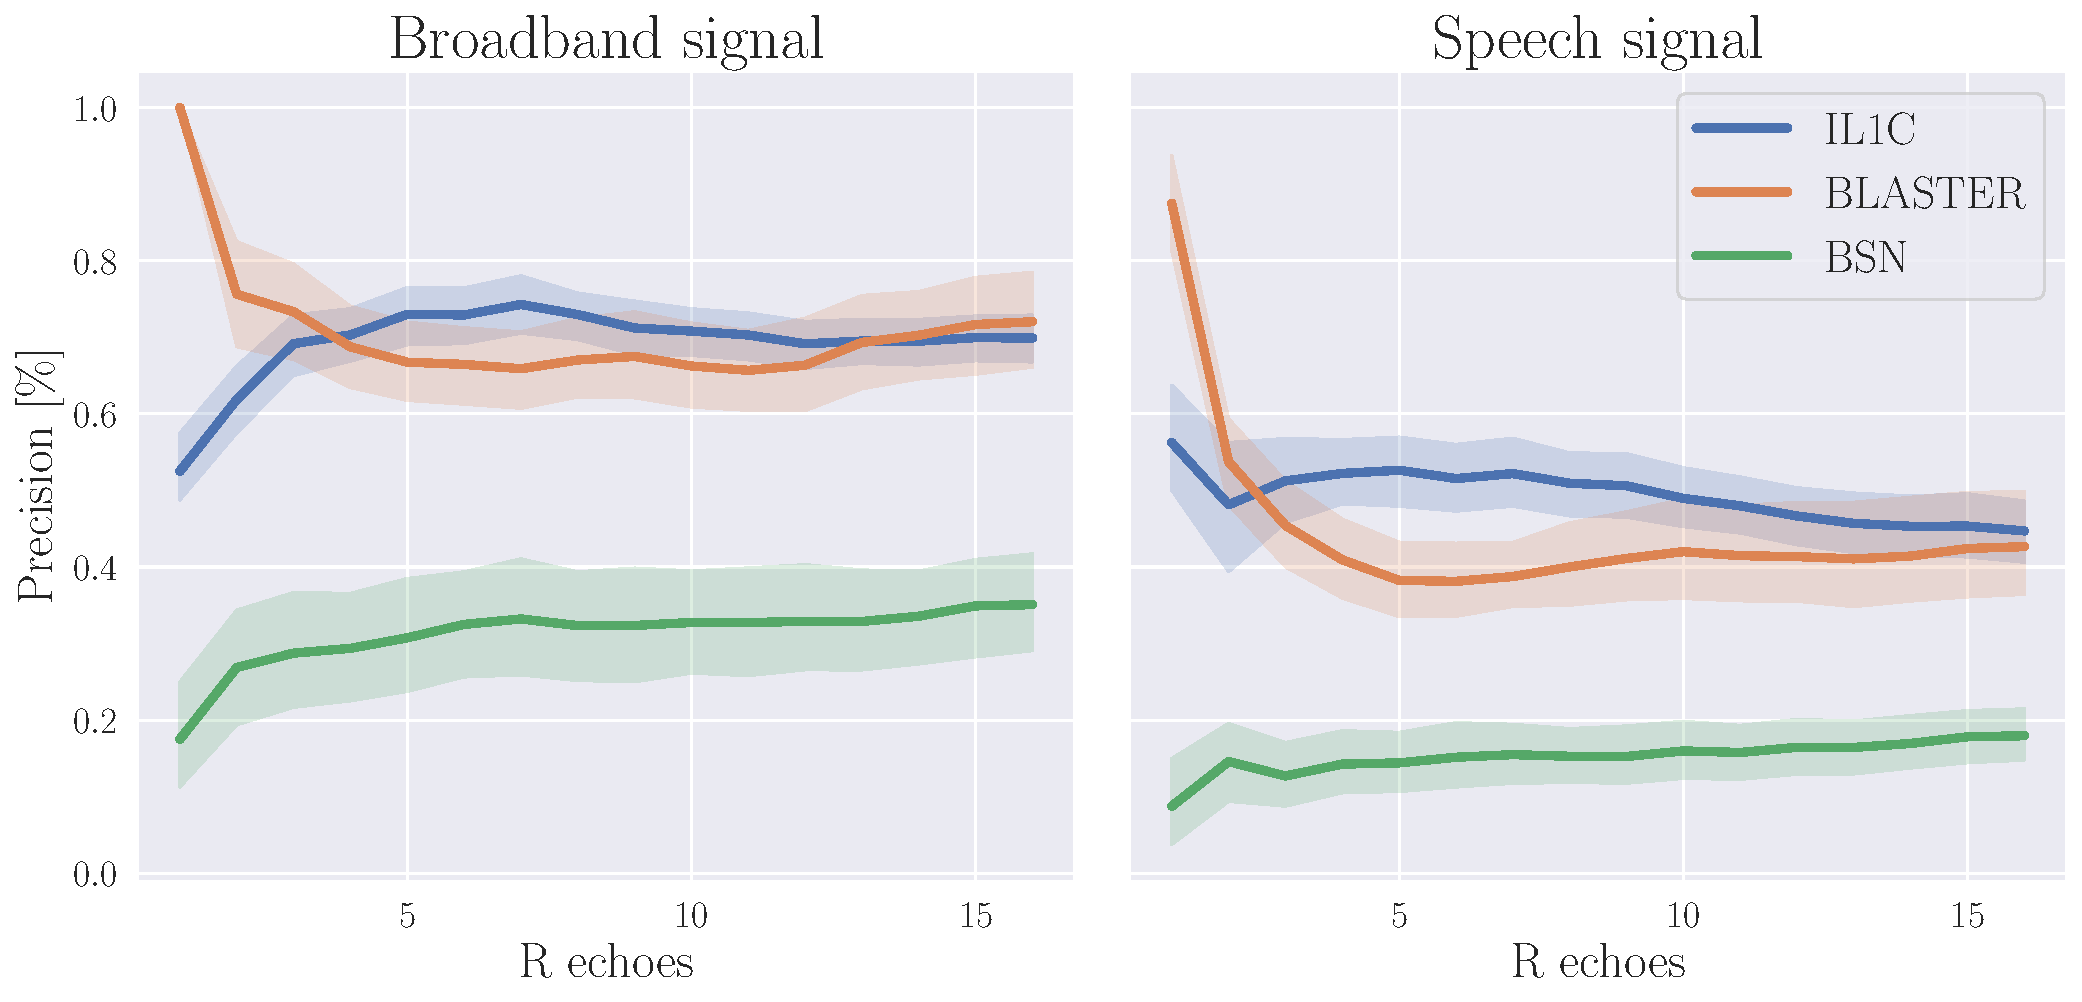
\includegraphics[width=\linewidth]{figures/p_k-7_thr-2_bns_crocco_blaster-peak_withRechoes.pdf}
%         \caption{\label{fig:error_precision_kecho}  Line plots with error bands of precision versus number of echoes $R$ to be retrieved for broadband (left) and speech (right) signals with \RT{} = $400$ ms and SNR = 20 dB.}
% \end{figure}





% Quantitative results are reported in Fig.~\ref{fig:error_precision_snr_rt}, Fig.~\ref{fig:error_precision_kecho} and Tab.~\ref{tab:error_precision_thr}. Here, for both RMSE and Precision and for both broadband and speech signal, the metrics are displayed against the dataset parameters. We observe that \algoBsn{} performs worst in all tested conditions, possibly due to its strong reliance on the peak picking step. For $R=7$ or higher, \algoBraire{} yields similar or slightly worse performance than \algoCrocco{} for the considered noise and reverberation levels, with decreasing performance for both as these levels increase. Using speech rather than broadband signals also yields worse results for all methods. However, the echo timing RMSE is significantly smaller using \algoBraire{} due to its off-grid advantage. We also note that \algoBraire{} significantly outperforms \algoCrocco{} on the task of recovering $R=2$ echoes. As showed in Tab.~\ref{tab:error_precision_thr}, in mild conditions, up to 68\% of echoes can be retrieved by \algoBraire{} with errors lower than half a sample in that case. This is promising since the practical advantage of knowing the timing of two echoes per channel has been demonstrated in~\cite{DiCarlo2019,Scheibler2017}.

% % Crocco-like short conclusion
% A novel blind, off-grid, multichannel echo retrieval method has been proposed based on the framework of continuous dictionaries.
% Comparisons with state-of-the-art approaches on various noise and reverberation conditions show that this method performs best when the number of echoes to retrieve is small.
% While some robustness to noise, reverberation, and non-broadband signals is observed, our experiments reveal that room for improvement exists for this challenging and emerging topic.
% Future works will include an extension to more than two channels and experiments on real-world data.

% \chapter{\lantern + \blaster = \blasterr}\label{chp:blasterr}



% %% III. Application
% \begin{fullwidth}
% \part{Echo-aware Application}\label{pt:application}
% \end{fullwidth}
% \parttoc[n]
% \chapter{Audio Scene Analysis meets Signal Processing}\label{ch:application}

\newthought{Synopsis} \synopsisChApplication

\mynewline
Here, we present some audio scene analysis problems that will be later discussed in their echo-aware extension.
Following the last part's structure, this introductory chapter gathers the common knowledge shared across the following ones.
Here we make a strong transition: we assume the echo properties are known a priori, so that the our focus is on the benefit of their knowledge.
The literature for each of them is reviewed, but since it is vast and spans diverse scientific research decades, we do not aim to cover it entirely.
Moreover, since the following chapters are dedicated to each of these problems under the echo-aware perspective, this specific literature is not considered here.
\\The material presented here results from the personal synthesis of concepts and references available in the literature.
Furthermore, some definitions are digested from classical textbooks already used for this thesis, such as~\citeonly{vincent2018audio}.

\section{Audio Scene Analysis Problems}\label{sec:application:scenario}
As mentioned in the first chapter, audio scene analysis aims to extract relevant information in the audio scene.
Different types of information are estimated or inferred by solving specific problems.
Despite their diversity, most of these problems can be defined with a common model.

\subsection{Common scenario and model}
Let there be a meeting room with well-defined geometry.
In it, $\numSrcs$ sound sources are located at determined positions, such as some speakers chatting while standing in the room, as in~\cref{fig:estimation:audioscene}.
As an indoor scenario, all the elements of reverberation (in particular echoes) are present.
Diffuse background noise is present as well, for instance, due to the air conditioner or car traffic outside.
This whole audio scene is recorded by a device featuring a microphone array of $\numMics$ sensors.
Furthermore we assume a static far field scenario and we model each $\idxSrc$ sources and $\idxMic$ microphone as well-defined points with coordinate $\positionSource$ and $\positionMicrophone$, respectively.
This is a reasonable assumption in the context of table-top devices, such as smart home devices.
\begin{figure}[]
    \begin{sidecaption}[Audio Scene]{%
        Illustration of an indoor audio scene recorded by three microphones.
        The microphone signals capture the reverberant mixture of several sound sources such as speech, music (guitar) and background diffuse noise (an air conditioner).
    }[fig:estimation:audioscene]
    \centering
    \resizebox{\linewidth}{!}{

\tikzset{every picture/.style={line width=0.75pt}} %set default line width to 0.75pt

\begin{tikzpicture}[x=0.75pt,y=0.75pt,yscale=-1,xscale=1]
%uncomment if require: \path (0,300); %set diagram left start at 0, and has height of 300

%Shape: Circle [id:dp37372160479593475]
\draw  [color={rgb, 255:red, 155; green, 155; blue, 155 }  ,draw opacity=0.76 ][line width=4.5]  (160,196) .. controls (160,184.95) and (168.95,176) .. (180,176) .. controls (191.05,176) and (200,184.95) .. (200,196) .. controls (200,207.05) and (191.05,216) .. (180,216) .. controls (168.95,216) and (160,207.05) .. (160,196) -- cycle ;
%Shape: Circle [id:dp6742469135937114]
\draw  [color={rgb, 255:red, 155; green, 155; blue, 155 }  ,draw opacity=0.76 ][line width=4.5]  (150,196) .. controls (150,179.43) and (163.43,166) .. (180,166) .. controls (196.57,166) and (210,179.43) .. (210,196) .. controls (210,212.57) and (196.57,226) .. (180,226) .. controls (163.43,226) and (150,212.57) .. (150,196) -- cycle ;
%Shape: Circle [id:dp6304501410818584]
\draw   (160,196) .. controls (160,184.95) and (168.95,176) .. (180,176) .. controls (191.05,176) and (200,184.95) .. (200,196) .. controls (200,207.05) and (191.05,216) .. (180,216) .. controls (168.95,216) and (160,207.05) .. (160,196) -- cycle ;
%Shape: Circle [id:dp6073489332662667]
\draw   (150,196) .. controls (150,179.43) and (163.43,166) .. (180,166) .. controls (196.57,166) and (210,179.43) .. (210,196) .. controls (210,212.57) and (196.57,226) .. (180,226) .. controls (163.43,226) and (150,212.57) .. (150,196) -- cycle ;
%Shape: Rectangle [id:dp5920548385374533]
\draw  [draw opacity=0][fill={rgb, 255:red, 255; green, 255; blue, 255 }  ,fill opacity=1 ] (130,230) -- (210,230) -- (210,250) -- (130,250) -- cycle ;
%Image [id:dp7339517530204356]
\draw (480,120) node  {
\includegraphics[width=10pt]{figures/acoustics/iconfinder_microphone_1608550.pdf}};
%Image [id:dp7608229391866312]
\draw (480,80) node  {
\includegraphics[width=10pt]{figures/acoustics/iconfinder_microphone_1608550.pdf}};
%Image [id:dp9664249278995992]
\draw (480,160) node  {
\includegraphics[width=10pt]{figures/acoustics/iconfinder_microphone_1608550.pdf}};
%Straight Lines [id:da6875965508418059]
\draw [color={rgb, 255:red, 245; green, 166; blue, 35 }  ,draw opacity=1 ]   (180,120) -- (467.03,80.41) ;
\draw [shift={(470,80)}, rotate = 532.15] [fill={rgb, 255:red, 245; green, 166; blue, 35 }  ,fill opacity=1 ][line width=0.08]  [draw opacity=0] (5.36,-2.57) -- (0,0) -- (5.36,2.57) -- cycle    ;
%Straight Lines [id:da21480429926103284]
\draw [color={rgb, 255:red, 245; green, 166; blue, 35 }  ,draw opacity=1 ]   (180,120) -- (467,120) ;
\draw [shift={(470,120)}, rotate = 180] [fill={rgb, 255:red, 245; green, 166; blue, 35 }  ,fill opacity=1 ][line width=0.08]  [draw opacity=0] (5.36,-2.57) -- (0,0) -- (5.36,2.57) -- cycle    ;
%Straight Lines [id:da6245847985271135]
\draw [color={rgb, 255:red, 245; green, 166; blue, 35 }  ,draw opacity=1 ]   (180,120) -- (467.03,159.59) ;
\draw [shift={(470,160)}, rotate = 187.85] [fill={rgb, 255:red, 245; green, 166; blue, 35 }  ,fill opacity=1 ][line width=0.08]  [draw opacity=0] (5.36,-2.57) -- (0,0) -- (5.36,2.57) -- cycle    ;
%Straight Lines [id:da7309183869115244]
\draw [color={rgb, 255:red, 0; green, 0; blue, 0 }  ,draw opacity=0.2 ] [dash pattern={on 4.5pt off 4.5pt}]  (220,80) -- (310,50) -- (467.05,79.45) ;
\draw [shift={(470,80)}, rotate = 190.62] [fill={rgb, 255:red, 0; green, 0; blue, 0 }  ,fill opacity=0.2 ][line width=0.08]  [draw opacity=0] (5.36,-2.57) -- (0,0) -- (5.36,2.57) -- cycle    ;
%Shape: Rectangle [id:dp15733721403583467]
\draw   (100,50) -- (560,50) -- (560,230) -- (100,230) -- cycle ;
%Straight Lines [id:da2249329781545223]
\draw [color={rgb, 255:red, 0; green, 0; blue, 0 }  ,draw opacity=0.6 ] [dash pattern={on 0.75pt off 0.75pt}]  (212.39,171.35) .. controls (213.1,169.1) and (214.58,168.33) .. (216.83,169.04) .. controls (219.08,169.75) and (220.55,168.98) .. (221.26,166.73) .. controls (221.97,164.48) and (223.44,163.71) .. (225.69,164.42) .. controls (227.94,165.13) and (229.42,164.36) .. (230.13,162.11) .. controls (230.84,159.86) and (232.31,159.09) .. (234.56,159.8) .. controls (236.81,160.5) and (238.28,159.73) .. (238.99,157.48) .. controls (239.7,155.23) and (241.18,154.46) .. (243.43,155.17) .. controls (245.68,155.88) and (247.15,155.11) .. (247.86,152.86) -- (249.44,152.04) -- (256.53,148.34) ;
\draw [shift={(259.19,146.95)}, rotate = 512.46] [fill={rgb, 255:red, 0; green, 0; blue, 0 }  ,fill opacity=0.6 ][line width=0.08]  [draw opacity=0] (5.36,-2.57) -- (0,0) -- (5.36,2.57) -- cycle    ;
%Straight Lines [id:da46872311549917245]
\draw [color={rgb, 255:red, 0; green, 0; blue, 0 }  ,draw opacity=0.6 ] [dash pattern={on 0.75pt off 0.75pt}]  (218.39,184.95) .. controls (219.88,183.12) and (221.54,182.95) .. (223.37,184.44) .. controls (225.2,185.93) and (226.86,185.75) .. (228.34,183.92) .. controls (229.82,182.09) and (231.48,181.91) .. (233.31,183.4) .. controls (235.14,184.89) and (236.8,184.71) .. (238.29,182.88) .. controls (239.78,181.05) and (241.43,180.88) .. (243.26,182.37) .. controls (245.09,183.86) and (246.75,183.68) .. (248.23,181.85) .. controls (249.72,180.02) and (251.38,179.84) .. (253.21,181.33) -- (257.45,180.89) -- (265.41,180.06) ;
\draw [shift={(268.39,179.75)}, rotate = 534.06] [fill={rgb, 255:red, 0; green, 0; blue, 0 }  ,fill opacity=0.6 ][line width=0.08]  [draw opacity=0] (5.36,-2.57) -- (0,0) -- (5.36,2.57) -- cycle    ;
%Straight Lines [id:da41740100207513164]
\draw [color={rgb, 255:red, 0; green, 0; blue, 0 }  ,draw opacity=0.6 ] [dash pattern={on 0.75pt off 0.75pt}]  (213.99,175.35) .. controls (214.96,173.2) and (216.52,172.61) .. (218.67,173.57) .. controls (220.82,174.54) and (222.38,173.94) .. (223.34,171.79) .. controls (224.3,169.64) and (225.86,169.04) .. (228.01,170.01) .. controls (230.16,170.98) and (231.72,170.38) .. (232.68,168.23) .. controls (233.65,166.08) and (235.21,165.48) .. (237.36,166.45) .. controls (239.51,167.42) and (241.07,166.82) .. (242.03,164.67) .. controls (242.99,162.52) and (244.55,161.92) .. (246.7,162.89) .. controls (248.85,163.86) and (250.41,163.26) .. (251.37,161.11) -- (254.11,160.07) -- (261.59,157.22) ;
\draw [shift={(264.39,156.15)}, rotate = 519.15] [fill={rgb, 255:red, 0; green, 0; blue, 0 }  ,fill opacity=0.6 ][line width=0.08]  [draw opacity=0] (5.36,-2.57) -- (0,0) -- (5.36,2.57) -- cycle    ;
%Straight Lines [id:da11925314169744539]
\draw [color={rgb, 255:red, 0; green, 0; blue, 0 }  ,draw opacity=0.6 ] [dash pattern={on 0.75pt off 0.75pt}]  (215.99,180.15) .. controls (217.24,178.16) and (218.87,177.78) .. (220.87,179.03) .. controls (222.87,180.28) and (224.49,179.91) .. (225.74,177.91) .. controls (226.99,175.91) and (228.61,175.54) .. (230.61,176.79) .. controls (232.61,178.04) and (234.23,177.67) .. (235.48,175.67) .. controls (236.73,173.67) and (238.36,173.3) .. (240.36,174.55) .. controls (242.36,175.8) and (243.98,175.42) .. (245.23,173.42) .. controls (246.48,171.42) and (248.1,171.05) .. (250.1,172.3) .. controls (252.1,173.55) and (253.72,173.18) .. (254.97,171.18) -- (255.67,171.02) -- (263.47,169.23) ;
\draw [shift={(266.39,168.55)}, rotate = 527.04] [fill={rgb, 255:red, 0; green, 0; blue, 0 }  ,fill opacity=0.6 ][line width=0.08]  [draw opacity=0] (5.36,-2.57) -- (0,0) -- (5.36,2.57) -- cycle    ;
%Straight Lines [id:da12240342341771249]
\draw [color={rgb, 255:red, 208; green, 2; blue, 27 }  ,draw opacity=1 ] [dash pattern={on 0.75pt off 0.75pt}]  (510,150) .. controls (509.26,152.24) and (507.77,152.99) .. (505.53,152.24) .. controls (503.3,151.49) and (501.81,152.24) .. (501.06,154.47) -- (499.84,155.08) -- (492.68,158.66) ;
\draw [shift={(490,160)}, rotate = 333.43] [fill={rgb, 255:red, 208; green, 2; blue, 27 }  ,fill opacity=1 ][line width=0.08]  [draw opacity=0] (5.36,-2.57) -- (0,0) -- (5.36,2.57) -- cycle    ;
%Straight Lines [id:da5418102098206483]
\draw [color={rgb, 255:red, 208; green, 2; blue, 27 }  ,draw opacity=1 ] [dash pattern={on 0.75pt off 0.75pt}]  (510,110) .. controls (509.26,112.24) and (507.77,112.99) .. (505.53,112.24) .. controls (503.3,111.49) and (501.81,112.24) .. (501.06,114.47) -- (499.84,115.08) -- (492.68,118.66) ;
\draw [shift={(490,120)}, rotate = 333.43] [fill={rgb, 255:red, 208; green, 2; blue, 27 }  ,fill opacity=1 ][line width=0.08]  [draw opacity=0] (5.36,-2.57) -- (0,0) -- (5.36,2.57) -- cycle    ;
%Straight Lines [id:da2263274179236877]
\draw [color={rgb, 255:red, 208; green, 2; blue, 27 }  ,draw opacity=1 ] [dash pattern={on 0.75pt off 0.75pt}]  (510,60) .. controls (509.26,62.24) and (507.77,62.99) .. (505.53,62.24) .. controls (503.3,61.49) and (501.81,62.24) .. (501.06,64.47) -- (499.84,65.08) -- (492.68,68.66) ;
\draw [shift={(490,70)}, rotate = 333.43] [fill={rgb, 255:red, 208; green, 2; blue, 27 }  ,fill opacity=1 ][line width=0.08]  [draw opacity=0] (5.36,-2.57) -- (0,0) -- (5.36,2.57) -- cycle    ;
%Straight Lines [id:da6407483239165986]
\draw [color={rgb, 255:red, 0; green, 0; blue, 0 }  ,draw opacity=0.2 ] [dash pattern={on 4.5pt off 4.5pt}]  (220,80) -- (350,230) -- (468.13,82.34) ;
\draw [shift={(470,80)}, rotate = 488.66] [fill={rgb, 255:red, 0; green, 0; blue, 0 }  ,fill opacity=0.2 ][line width=0.08]  [draw opacity=0] (5.36,-2.57) -- (0,0) -- (5.36,2.57) -- cycle    ;
%Straight Lines [id:da5328192505993826]
\draw [color={rgb, 255:red, 0; green, 0; blue, 0 }  ,draw opacity=0.2 ] [dash pattern={on 4.5pt off 4.5pt}]  (220,80) -- (330,50) -- (467.32,118.66) ;
\draw [shift={(470,120)}, rotate = 206.57] [fill={rgb, 255:red, 0; green, 0; blue, 0 }  ,fill opacity=0.2 ][line width=0.08]  [draw opacity=0] (5.36,-2.57) -- (0,0) -- (5.36,2.57) -- cycle    ;
%Straight Lines [id:da8377831024194228]
\draw [color={rgb, 255:red, 0; green, 0; blue, 0 }  ,draw opacity=0.2 ] [dash pattern={on 4.5pt off 4.5pt}]  (220,80) -- (370,230) -- (468.34,82.5) ;
\draw [shift={(470,80)}, rotate = 483.69] [fill={rgb, 255:red, 0; green, 0; blue, 0 }  ,fill opacity=0.2 ][line width=0.08]  [draw opacity=0] (5.36,-2.57) -- (0,0) -- (5.36,2.57) -- cycle    ;
%Straight Lines [id:da38697516677735044]
\draw [color={rgb, 255:red, 0; green, 0; blue, 0 }  ,draw opacity=0.2 ] [dash pattern={on 4.5pt off 4.5pt}]  (220,80) -- (400,230) -- (467.88,162.12) ;
\draw [shift={(470,160)}, rotate = 495] [fill={rgb, 255:red, 0; green, 0; blue, 0 }  ,fill opacity=0.2 ][line width=0.08]  [draw opacity=0] (5.36,-2.57) -- (0,0) -- (5.36,2.57) -- cycle    ;
%Image [id:dp4512377721787463]
\draw (200,80) node  {
\includegraphics[width=30pt]{figures/speech.pdf}};
%Image [id:dp11655856762581418]
\draw (160,120) node  {
\includegraphics[width=45pt]{figures/guitar.pdf}};
%Straight Lines [id:da6506133051173556]
\draw [color={rgb, 255:red, 0; green, 0; blue, 0 }  ,draw opacity=0.6 ] [dash pattern={on 0.75pt off 0.75pt}]  (218.06,191.95) .. controls (219.65,190.21) and (221.31,190.13) .. (223.05,191.72) .. controls (224.8,193.31) and (226.46,193.23) .. (228.05,191.48) .. controls (229.64,189.74) and (231.3,189.66) .. (233.04,191.25) .. controls (234.78,192.84) and (236.45,192.76) .. (238.04,191.02) .. controls (239.62,189.27) and (241.28,189.19) .. (243.03,190.78) .. controls (244.77,192.37) and (246.44,192.29) .. (248.03,190.55) .. controls (249.61,188.8) and (251.27,188.72) .. (253.02,190.31) -- (257.45,190.1) -- (265.44,189.73) ;
\draw [shift={(268.43,189.59)}, rotate = 537.31] [fill={rgb, 255:red, 0; green, 0; blue, 0 }  ,fill opacity=0.6 ][line width=0.08]  [draw opacity=0] (5.36,-2.57) -- (0,0) -- (5.36,2.57) -- cycle    ;
%Straight Lines [id:da9912250072749541]
\draw [color={rgb, 255:red, 245; green, 166; blue, 35 }  ,draw opacity=0.3 ] [dash pattern={on 4.5pt off 4.5pt}]  (180,120) -- (290,230) -- (467.7,81.92) ;
\draw [shift={(470,80)}, rotate = 500.19] [fill={rgb, 255:red, 245; green, 166; blue, 35 }  ,fill opacity=0.3 ][line width=0.08]  [draw opacity=0] (5.36,-2.57) -- (0,0) -- (5.36,2.57) -- cycle    ;
%Straight Lines [id:da842755271595558]
\draw [color={rgb, 255:red, 245; green, 166; blue, 35 }  ,draw opacity=0.3 ] [dash pattern={on 4.5pt off 4.5pt}]  (180,120) -- (310,230) -- (467.53,121.7) ;
\draw [shift={(470,120)}, rotate = 505.49] [fill={rgb, 255:red, 245; green, 166; blue, 35 }  ,fill opacity=0.3 ][line width=0.08]  [draw opacity=0] (5.36,-2.57) -- (0,0) -- (5.36,2.57) -- cycle    ;
%Straight Lines [id:da565897385867932]
\draw [color={rgb, 255:red, 245; green, 166; blue, 35 }  ,draw opacity=0.3 ] [dash pattern={on 4.5pt off 4.5pt}]  (180,120) -- (340,230) -- (467.36,161.42) ;
\draw [shift={(470,160)}, rotate = 511.7] [fill={rgb, 255:red, 245; green, 166; blue, 35 }  ,fill opacity=0.3 ][line width=0.08]  [draw opacity=0] (5.36,-2.57) -- (0,0) -- (5.36,2.57) -- cycle    ;
%Straight Lines [id:da016277657003535784]
\draw [color={rgb, 255:red, 0; green, 0; blue, 0 }  ,draw opacity=0.6 ] [dash pattern={on 0.75pt off 0.75pt}]  (215.77,214.66) .. controls (218.07,214.14) and (219.48,215.03) .. (219.99,217.33) .. controls (220.51,219.63) and (221.92,220.52) .. (224.22,220.01) .. controls (226.52,219.49) and (227.93,220.38) .. (228.44,222.68) .. controls (228.95,224.98) and (230.36,225.87) .. (232.66,225.35) .. controls (234.96,224.84) and (236.37,225.73) .. (236.89,228.03) -- (240,230) -- (240,230) .. controls (240.17,227.65) and (241.44,226.56) .. (243.79,226.74) .. controls (246.14,226.92) and (247.41,225.83) .. (247.58,223.48) .. controls (247.76,221.13) and (249.03,220.04) .. (251.38,220.22) .. controls (253.73,220.4) and (255,219.31) .. (255.17,216.96) .. controls (255.34,214.61) and (256.61,213.52) .. (258.96,213.7) -- (260.76,212.16) -- (266.82,206.94) ;
\draw [shift={(269.1,204.99)}, rotate = 499.32] [fill={rgb, 255:red, 0; green, 0; blue, 0 }  ,fill opacity=0.6 ][line width=0.08]  [draw opacity=0] (5.36,-2.57) -- (0,0) -- (5.36,2.57) -- cycle    ;
%Straight Lines [id:da9867855512078149]
\draw [color={rgb, 255:red, 0; green, 0; blue, 0 }  ,draw opacity=0.6 ] [dash pattern={on 0.75pt off 0.75pt}]  (218.1,207.99) .. controls (220.42,207.56) and (221.79,208.51) .. (222.22,210.83) .. controls (222.64,213.15) and (224.01,214.1) .. (226.33,213.67) .. controls (228.65,213.24) and (230.02,214.19) .. (230.45,216.51) .. controls (230.87,218.83) and (232.24,219.78) .. (234.56,219.35) .. controls (236.88,218.92) and (238.25,219.87) .. (238.68,222.19) .. controls (239.1,224.51) and (240.47,225.46) .. (242.79,225.03) .. controls (245.11,224.6) and (246.48,225.55) .. (246.91,227.87) -- (250,230) -- (250,230) .. controls (250.29,227.66) and (251.6,226.63) .. (253.94,226.92) .. controls (256.28,227.21) and (257.59,226.18) .. (257.88,223.84) .. controls (258.17,221.5) and (259.48,220.48) .. (261.82,220.77) .. controls (264.16,221.06) and (265.47,220.03) .. (265.76,217.69) -- (266.1,217.43) -- (272.4,212.5) ;
\draw [shift={(274.77,210.66)}, rotate = 502.01] [fill={rgb, 255:red, 0; green, 0; blue, 0 }  ,fill opacity=0.6 ][line width=0.08]  [draw opacity=0] (5.36,-2.57) -- (0,0) -- (5.36,2.57) -- cycle    ;
%Straight Lines [id:da5055644084768178]
\draw [color={rgb, 255:red, 0; green, 0; blue, 0 }  ,draw opacity=0.6 ] [dash pattern={on 0.75pt off 0.75pt}]  (210,220.33) .. controls (212.23,219.59) and (213.72,220.34) .. (214.47,222.57) .. controls (215.21,224.81) and (216.7,225.56) .. (218.94,224.81) .. controls (221.17,224.06) and (222.67,224.81) .. (223.42,227.04) .. controls (224.16,229.28) and (225.65,230.03) .. (227.89,229.28) -- (230,230.33) -- (230,230.33) .. controls (230.17,227.98) and (231.44,226.9) .. (233.79,227.07) .. controls (236.14,227.25) and (237.41,226.16) .. (237.58,223.81) .. controls (237.75,221.46) and (239.02,220.37) .. (241.37,220.55) .. controls (243.72,220.73) and (244.99,219.64) .. (245.16,217.29) .. controls (245.33,214.94) and (246.6,213.85) .. (248.95,214.03) .. controls (251.3,214.21) and (252.57,213.12) .. (252.74,210.77) -- (255.76,208.16) -- (261.83,202.95) ;
\draw [shift={(264.1,200.99)}, rotate = 499.29] [fill={rgb, 255:red, 0; green, 0; blue, 0 }  ,fill opacity=0.6 ][line width=0.08]  [draw opacity=0] (5.36,-2.57) -- (0,0) -- (5.36,2.57) -- cycle    ;
%Straight Lines [id:da5832987622194876]
\draw [color={rgb, 255:red, 0; green, 0; blue, 0 }  ,draw opacity=0.2 ] [dash pattern={on 4.5pt off 4.5pt}]  (220,80) -- (350,50) -- (467.79,157.97) ;
\draw [shift={(470,160)}, rotate = 222.51] [fill={rgb, 255:red, 0; green, 0; blue, 0 }  ,fill opacity=0.2 ][line width=0.08]  [draw opacity=0] (5.36,-2.57) -- (0,0) -- (5.36,2.57) -- cycle    ;
%Straight Lines [id:da5008400993643431]
\draw [color={rgb, 255:red, 245; green, 166; blue, 35 }  ,draw opacity=0.3 ] [dash pattern={on 4.5pt off 4.5pt}]  (180,120) -- (350,50) -- (467.79,157.97) ;
\draw [shift={(470,160)}, rotate = 222.51] [fill={rgb, 255:red, 245; green, 166; blue, 35 }  ,fill opacity=0.3 ][line width=0.08]  [draw opacity=0] (5.36,-2.57) -- (0,0) -- (5.36,2.57) -- cycle    ;
%Straight Lines [id:da2480092091139493]
\draw [color={rgb, 255:red, 245; green, 166; blue, 35 }  ,draw opacity=0.3 ] [dash pattern={on 4.5pt off 4.5pt}]  (180,120) -- (370,50) -- (467.54,118.28) ;
\draw [shift={(470,120)}, rotate = 214.99] [fill={rgb, 255:red, 245; green, 166; blue, 35 }  ,fill opacity=0.3 ][line width=0.08]  [draw opacity=0] (5.36,-2.57) -- (0,0) -- (5.36,2.57) -- cycle    ;
%Straight Lines [id:da98913951227942]
\draw [color={rgb, 255:red, 245; green, 166; blue, 35 }  ,draw opacity=0.3 ] [dash pattern={on 4.5pt off 4.5pt}]  (180,120) -- (400,50) -- (467.24,78.82) ;
\draw [shift={(470,80)}, rotate = 203.2] [fill={rgb, 255:red, 245; green, 166; blue, 35 }  ,fill opacity=0.3 ][line width=0.08]  [draw opacity=0] (5.36,-2.57) -- (0,0) -- (5.36,2.57) -- cycle    ;
%Straight Lines [id:da7940761686938484]
\draw [color={rgb, 255:red, 74; green, 74; blue, 74 }  ,draw opacity=1 ]   (220,80) -- (467,80) ;
\draw [shift={(470,80)}, rotate = 180] [fill={rgb, 255:red, 74; green, 74; blue, 74 }  ,fill opacity=1 ][line width=0.08]  [draw opacity=0] (5.36,-2.57) -- (0,0) -- (5.36,2.57) -- cycle    ;
%Straight Lines [id:da03582329188397548]
\draw [color={rgb, 255:red, 74; green, 74; blue, 74 }  ,draw opacity=1 ]   (220,80) -- (467.04,119.53) ;
\draw [shift={(470,120)}, rotate = 189.09] [fill={rgb, 255:red, 74; green, 74; blue, 74 }  ,fill opacity=1 ][line width=0.08]  [draw opacity=0] (5.36,-2.57) -- (0,0) -- (5.36,2.57) -- cycle    ;
%Straight Lines [id:da5309831276841109]
\draw [color={rgb, 255:red, 74; green, 74; blue, 74 }  ,draw opacity=1 ]   (220,80) -- (467.14,159.09) ;
\draw [shift={(470,160)}, rotate = 197.74] [fill={rgb, 255:red, 74; green, 74; blue, 74 }  ,fill opacity=1 ][line width=0.08]  [draw opacity=0] (5.36,-2.57) -- (0,0) -- (5.36,2.57) -- cycle    ;
%Image [id:dp7579313396430111]
\draw (180,196) node  {
\includegraphics[width=18.75pt]{figures/ac.pdf}};
%Straight Lines [id:da14142044437195245]
\draw    (480,90) -- (577,90) ;
\draw [shift={(580,90)}, rotate = 180] [fill={rgb, 255:red, 0; green, 0; blue, 0 }  ][line width=0.08]  [draw opacity=0] (7.14,-3.43) -- (0,0) -- (7.14,3.43) -- (4.74,0) -- cycle    ;
%Straight Lines [id:da0847611097781068]
\draw    (480,130) -- (577,130) ;
\draw [shift={(580,130)}, rotate = 180] [fill={rgb, 255:red, 0; green, 0; blue, 0 }  ][line width=0.08]  [draw opacity=0] (7.14,-3.43) -- (0,0) -- (7.14,3.43) -- (4.74,0) -- cycle    ;
%Straight Lines [id:da009579756930902739]
\draw    (480,170) -- (577,170) ;
\draw [shift={(580,170)}, rotate = 180] [fill={rgb, 255:red, 0; green, 0; blue, 0 }  ][line width=0.08]  [draw opacity=0] (7.14,-3.43) -- (0,0) -- (7.14,3.43) -- (4.74,0) -- cycle    ;

% Text Node
\draw (467,95.4) node [anchor=north west][inner sep=0.75pt]  [font=\footnotesize]  {$\positionMicrophone_{1}$};
% Text Node
\draw (467,135.4) node [anchor=north west][inner sep=0.75pt]  [font=\footnotesize]  {$\positionMicrophone_{2}$};
% Text Node
\draw (467,175.4) node [anchor=north west][inner sep=0.75pt]  [font=\footnotesize]  {$\positionMicrophone_{3}$};
% Text Node
\draw (577,76.4) node [anchor=north west][inner sep=0.75pt]  [font=\footnotesize]  {$\mic_{1}$};
% Text Node
\draw (577,116.4) node [anchor=north west][inner sep=0.75pt]  [font=\footnotesize]  {$\mic_{2}$};
% Text Node
\draw (577,156.4) node [anchor=north west][inner sep=0.75pt]  [font=\footnotesize]  {$\mic_{3}$};
% Text Node
\draw (221,65.4) node [anchor=north west][inner sep=0.75pt]  [font=\footnotesize]  {$\src_{1}$};
% Text Node
\draw (204,101.4) node [anchor=north west][inner sep=0.75pt]  [font=\footnotesize]  {$\positionSource_{1}$};
% Text Node
\draw (171,117.4) node [anchor=north west][inner sep=0.75pt]  [font=\footnotesize,color={rgb, 255:red, 245; green, 166; blue, 35 }  ,opacity=1 ]  {$\src_{2}$};
% Text Node
\draw (151,149.4) node [anchor=north west][inner sep=0.75pt]  [font=\footnotesize,color={rgb, 255:red, 245; green, 166; blue, 35 }  ,opacity=1 ]  {$\positionSource_{2}$};
% Text Node
\draw (201,160.4) node [anchor=north west][inner sep=0.75pt]  [font=\footnotesize,color={rgb, 255:red, 128; green, 128; blue, 128 }  ,opacity=1 ]  {$\nse$};


\end{tikzpicture}
}
    \end{sidecaption}
\end{figure}
Recalling the (discrete) time-domain signal model already discussed in~\cref{subsec:processing:mixing}, the signal recorded at the $\idxMic$-th microphones reads
\begin{equation}
    \label{eq:application:mix}
    \mic_\idxMic[n] = \sum_{\idxSrc = 1}^{\numSrcs}
        \kparen{\flt_{\idxMicSrc}( \positionMicrophone_{\idxMic}  | \positionSource_{\idxSrc}) \convDis \src_{\idxSrc}} [n] + \nse_\idxMic[n]
    ,
\end{equation}
or alternatively, using the source spatial image signals,
\begin{equation}
    \label{eq:application:mix_img}
    \begin{aligned}
        \img_{\idxMicSrc}[n]  &= \kparen{\flt_{\idxMicSrc}( \positionMicrophone_{\idxMic}  | \positionSource_{\idxSrc}) \convDis \src_{\idxSrc}}[n]
        \mic_\idxMic[n]     &= \sum_{\idxSrc = 1}^{\numSrcs} \img_{\idxMicSrc}[n] + \nse_\idxMic[n],\\
        .
    \end{aligned}
\end{equation}
Note that the filter $\flt_{\idxMicSrc}(\positionMicrophone_{\idxMic} | \positionSource_{\idxSrc})$ denotes the \RIR/ where we intentionally highlight the dependencies on geometry,
namely, accounting for the whole sound propagation for the source position $\positionSource_{\idxSrc}$ to the microphone position $\positionMicrophone_{\idxMic}$.
In fact, as discussed throughout~\cref{pt:background}, we can decouple the information of indoor microphone natural recordings into two orthogonal contributions:
the \RIRs/ (thus the mixing matrix) accounting for only the sound propagation, and the source signals describes only the semantic content.

\newcommand{\setMicSignals}{\ensuremath{\set{\mic_{\idxMic}}_\idxMic}}
\newcommand{\setSrcSignals}{\ensuremath{\set{\src_{\idxSrc}}_\idxSrc}}
\newcommand{\setSrcPositions}{\ensuremath{\set{\positionSource_{\idxSrc}}_\idxSrc}}
\newcommand{\setFltSignals}{\ensuremath{\set{\flt_{\idxMicSrc}(\positionMicrophone_{\idxMic} | \positionSource_{\idxSrc})}_{\idxMicSrc}}}


\subsection{Problem formulation}
The Audio Scene Analysis Problems presented already in the introductory chapter (See~\cref{sec:intro:scene}) can now be extended and rewritten in terms of the above notation.
Furthermore, we will consider here the only ones directly addressed in this thesis: room impulse response estimation, audio source separation, Spatial filtering, sound source localization, and room geometry estimation.

\begin{table}[!h]

    \begin{fullwidth}
    \centering
    \small
    \renewcommand{\arraystretch}{1.3}

    \begin{tabular*}{\linewidth}{@{\extracolsep{\fill}}lllll@{}}
    \toprule
    Audio scene analysis problems & \textit{from the mixtures $\setMicSignals$, can we estimate...}  & Chapter\\
    \midrule

    Audio Source Separation     & \begin{tabular}[c]{@{}l@{}}the source signals $\setSrcSignals$ and\\ \hspace{1em} the filters $\setFltSignals$?\end{tabular}   & \cref{ch:separake}\\

    Spatial filtering           & \begin{tabular}[c]{@{}l@{}}the source signals $\setSrcSignals$,\\ \hspace{1em} knowing the filters $\setFltSignals$?\end{tabular} & \cref{ch:decharateapp}~\cref{sec:dechorateapp:se}\\

    Sound Source Localization   & the source positions $\setSrcPositions$?                              & \cref{ch:mirage}\\

    Room Geometry Estimation    & the shape of the room?                                                & \cref{ch:decharateapp}~\cref{sec:dechorateapp:rooge}\\
    \bottomrule
\end{tabular*}


% Channel (or \RIR/) Estimation            & the filters $\setFltSignals$ ?                            & \cref{pt:estimation}\\

% Acoustic Echo Retrieval     & the early echoes' timings and gain accounted in $\setFltSignals$ ?     & \cref{pt:estimation}\\

% \RIR/ measurement           & the filters $\setFltSignals$, knowing $\setSrcSignals$ ?               & \cref{ch:dechorate}\\
% Speech Enhancement          & the signal of the $\idxSrc$-th target source $\src_{\idxSrc}$?        & \cref{ch:decharateapp}\\

    % \hline

    \caption{List of audio scene analysis problems considered in this thesis accompanied by their mathematical description.}
    \label{tab:application:problems}

    \end{fullwidth}

\end{table}

\mynewline
As introduced in~\cref{sec:estimation:problem}, these problems can be said either \textit{informed} or \textit{blind} and the related scenario \textit{active} or \textit{passive}.
These two dichotomies emphasize the amount of prior knowledge available for solving them.
As opposed to the active scenario, where the source signal is known, transmitted, and available, the passive one considers only the microphone measurements.
For instance, when addressing the active echo estimation problem or \RIR/ measurement, the exact time of emission of the source signal is known, as well as the source signal itself.
\\The second dichotomy refers to the possibility of exploiting prior knowledge to solve the problem more easily.
This information may derive from annotations and meta-data.
In the community of audio source separation, the following definitions were proposed in~\citeonly{vincent2014blind}:
as opposed to informed problems, for solving the blind ones, absolutely no information is given about the source signal or the mixing process.
In between, there are \textit{semi-blind} or \textit{guided} problems:
here general information is available, such as on the nature of the source signal (speech, music, environmental sounds),
microphone position, recording scenario (indoor, outdoor, professional music), mixing process, \etc/.
In some books and works other categories of problems are defined, such as \emph{weakly-guided}, \emph{strongly-guided}.
Here we do not consider these distinctions.

\mynewline
In the considered echo-aware applications, the echoes properties build our prior knowledge on the problem.
Therefore, according to the above taxonomy, the addressed problems are necessarily guided.
In general and unless specified, this is the only knowledge we will assume to have.
Based on this, we will now review some classical works for solving the above problems.


\newthought{In the following sections} we will present the general overview of the literature related to the problems considered in this thesis: multichannel audio source separation, Spatial filtering, and sound source localization.
We will limit the discussion to the most relevant techniques adopted nowadays with respect to the acoustic propagation modeling.
Later in the thesis, dedicated sections on echo-aware method to address these problems will be provided in each related chapter.
Since room geometry estimation is mainly based on echo estimation and labeling discussed in~\cref{subsec:estimation:active_rir}, its description is postponed to~\cref{sec:dechorateapp:rooge}.


\section{Overview on multichannel Sound Source Separation}\label{sec:application:separation}
Multichannel audio source separation refers to the process of extracting acoustic signals from multichannel mixtures featuring targets, interfering, and noisy sounds.
In psychoacoustics, this problem is known as \textit{the cocktail party problem}~\citeonly{cherry1953cocktail}, referring to the human ability to focus on a particular stimulus in a audio scene.
This problem has interested mainly in two research fields in the audio signal processing community: speech and music processing.
Both share many methods, which are accordingly modified, taking into account scenarios and applications.
\marginpar{
    \footnotesize\itshape
    Many other methods have been proposed in the literature.
    The reader can refer to \citeonly{vincent2018audio, makino2018audio}
}
In the context of the multichannel speech recordings, some of the most successful and popular methods used nowadays
include Spatial filtering, \TF/ masking, and end-to-end regression.
In this thesis, we deliberately distinguish between the Spatial filtering, which will be discussed in the following subsection, and \TF/ masking.
\\\TF/ masking relies on \TF/ diversity of the sources and processes each mixture channel separately.
In a nutshell, it involves computing the \acp{STFT} of the mixture channels, multiplying them by masks containing gains between 0 and 1.
One of the most popular masking rules is adaptive Wiener filtering.
For each time-frequency bin, the \acp{STFT} of the estimated source spatial images $\IMG_{\idxMicSrc}$ of the $\idxSrc$-th source at the $\idxMic$ microphone, writes
\begin{equation}
        \hat{\IMG}_{\idxMicSrc} = \underbrace{\frac{\powerOf{\IMG_{\idxMicSrc}}}
                                        {\sum_{\idxSrc=0}^\numSrcs \powerOf{\IMG_{\idxMicSrc}}}}
                                        _{\text{Wiener filter}} \; \MIC_\idxMic
\end{equation}
where $\MIC_\idxMic$ is the \STFT/ of the microphone channel. Here the \TF/ bin is omitted for clarity.
\\In order to be computed, the Wiener filter requires estimating all the source spatial images, or equivalently, the mixing filters and the source signals.
Therefore, this approach has been generalized in several ways to account for both these unknowns.
In these thesis we stress the difference between source separation and Spatial filtering.
In the former, all the source signals and mixing filters are indispensable to weigh each of the \TF/ bins of the microphone channel's \STFT/.
As opposed to, in the latter problem, the ``masks'', that is the spatial filters, are estimate only based the mixing filters and noise statistics.
In multichannel recordings, a clear overlap exist between the two problems, and some techniques can be used reciprocally.
Furthermore the related research trends are now converging under the same umbrella of the so-called \textit{speech enhancement}.
The work~\citeonly{gannot2017consolidated} provide an unified framework merging source separation and Spatial filtering.
Nevertheless, we will treat them as separated problems.

\mynewline
Moreover, the benefit of the \TF/ masking approach is that the masks can be estimated in various ways.
For instance, clustering and classification techniques~\citeonly{rickard2007duet} can be used to assign each \TF/-bin to each of the sources.
Recently learning-based methods have been used in this sense on the same task~\citeonly{hershey2016deep,wang2018multi}.
Alternatively, deep learning techniques can used to directly estimated the sources' \TF/, as done in one of the reference implementation~\citeonly{stoter2019open}.
The work of \citeonly{nugraha2016multichannel}, instead, uses a deep learning model build by unfolding the the popular Multichannel \ac{NMF} source separation framework of~\citeonly{ozerov2010multichannel, sawada2013multichannel}.

\mynewline
The Gaussian-based Multichannel \ac{NMF}~\citeonly{ozerov2010multichannel} is one of the most successful framework for source separation using \TF/ masks.
It combines the \ac{NMF} and narrowband spatial model (discussed in ~\cref{subsec:processing:model:stft}) and deploys optimization-based framework for estimating both the mixing matrix and the sources.
One of the main advantage of this approach is that it allows to easily incorporated prior knowledge on the problem.
Thanks to the narrowband approximation (\cref{eq:processing:narrow}), spatial and semantic content are orthogonal and can be treated disjointedly.
This opens to many possibilities, such as, using pre-trained dictionaries to model source content~\citeonly{schmidt2006single, smaragdis2009sparse}, or using proper model for the mixing filters, such as \RIRs/, steering vectors, \ReTFs/, \etc/.

\mynewline
However, it has been shown that even with oracle \TF/~\citeonly{luo2019conv}, the estimation is still affected by artifacts.
This limitation affects all the approaches operating in the \TF/ domain.
To overcome this, end-to-deep deep learning models~\citeonly{luo2019conv, tzinis2020sudo} were developed and now hold the record in source separation.
These models work directly in the time domain: both input and output are time-domain waveforms.
This approach has prove to reach good separation quality, especially in terms of perceived sounds at the listener.
Nevertheless, all deep learning methods rely on trained black-box models for which is hard to inject prior knowledge.
Instead, Multichannel NMF-based frameworks accounts for this freedom.

\subsection{Multichannel NMF source separation}
Multichannel NMF source separation methods can be grouped according to how they model sound propagation of the mixing process:
\begin{itemize}
    \item those that simply ignore it \citeonly{le2015deep};
    \item (\textit{free field propagation}) those that assume a single anechoic path \citeonly{rickard2007duet, nesta2012convolutive} ;
    \item (\textit{reverberant propagation}) those that model the \RTFs/ entirely \citeonly{ozerov2010multichannel, duong2010under, li2019expectation};
    \item (\textit{reverberant propagation}) and those that attempt to separately estimate the contribution of the early echoes and the contribution of the late tail \citeonly{leglaive2015multichannel}.
\end{itemize}
Therefore, these existing approaches either ignore sound propagation or aim at estimating it fully, which affect the quality of the separation.
In the first case, strong echoes and reverberant constitute a low bound in the separation capability.
In fact, these elements of the sound propagation blur and spread the energy of the source source over multiple \TF/ bins, for which the assignation is harder.
When computing the \TF/ masking operation, these bins may introduce strong artifacts.
In the second case, the algorithm need to estimated more parameters with consequences in complexity and estimation accuracy.

\newthought{Echo-aware source separation methods} have been introduced as a possible solution to overcome some of these limitations,.
More details will be given in~\cref{ch:separake}, where a new method for speech source separation based on the Multichannel \NMF/ framework and echoes is described.

\section{Overview on Spatial filtering}\label{sec:application:filtering}\marginpar{
    \footnotesize\itshape
    For a comprehensive review on Spatial filtering methods, the reader can refer to the book~\citeonly{VanTrees2004Optimum}.
}
Spatial filtering aim at the enhancement of a desired signal while suppressing the background noise and/or interfering signals.
It is a large and active research field that has interested the signal processing and telecommunication communities since several decades.
It has produced an vast literature including several reference books dedicated to the topic.
For more details in this direction, the reader can refers to, e.g., the book~\citeonly{VanTrees2004Optimum}.
In audio, this topic was been extensively review in the context of speech enhancement in a recent publication~\citeonly{gannot2017consolidated}\sidenote{
    The content of this work has been extended in the book~\citeonly{vincent2018audio}.
}

\mynewline
In Spatial filtering, the \RIRs/ (and related models, \eg/, \RTFs/, steering vectors or \ReTFs/) play a central role.
Intuitively, giving the mixing model in~\cref{eq:application:mix}, the enhancement of a target source can be achieved by merely denoising the recordings and filtering by the inverting \RIRs/.
However, this is not always possible as the inversion of the \RIRs/ is not a straightforward operation.
The work in~\citeonly{neely1979invertibility} discuss explicitly the issues of inverting \RIRs/.
Later, several techniques were investigated, which are sometimes referred to as Room Response \textit{Equalization}~\citeonly{cecchi2018room}.
% First, there is a fundamental trade-off between denoising and filtering capabilities, which are related to the number of degree of freedom imposed by the number of microphones available~\citeonly{VanTrees2004Optimum}
% They can be exhausted by imposing unit- and null-gain directions constraints


\subsection{Beamforming}
Beamforming is one of the most famous techniques used in Spatial filtering.
One of the most famous beamformer is the \ac{DS}.
The intuitive idea behind it is to sum the microphone channels constructively by compensating the time delays between the sound source and the spatially separated microphones.
Thus, the target source signal is enhanced, while noise, interferences, and reverberation being suppressed.
\cref{fig:application:ds} illustrate this ideas.
Later, this idea has been extended to Frequency and Time-Frequency processing with direct modeling of the noise sources.
More formally, beamformers design mathematical \textit{optimization criterion}, namely objective function, defining the desired shape of the estimated signal and return a filter to be applied to the microphone recordings.
For instance, one may want to keep a unit gain towards the desired sound source's direction while minimizing the sounds from all the other directions.
The literature on beamformers spans in two directions: different optimization criteria and how to estimate the parameters required by their computation.
We will now elaborate the two directions in turn.
\begin{figure}
    \begin{sidecaption}[]{
        Illustration of the \ac{DS} Beamforming in the time-domain applied to a pulse source signal.
        The delays of the recorded signals at each microphone are compensated.
        By summing the shifted signals, the source signal is enhanced.
        Image courtesy of Robin Scheibler, author of ~\citeonly{scheibler2015raking}.
    }[fig:application:ds]
        \centering
        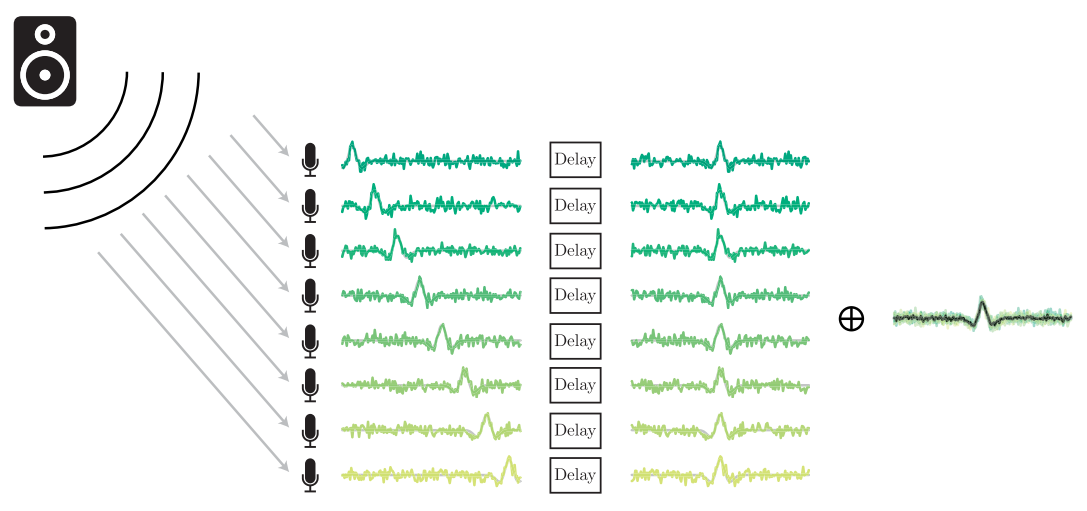
\includegraphics[width=\linewidth]{application/ds.png}
    \end{sidecaption}
\end{figure}

\newthought{Many beamformers criteria} have been proposed.
Among all, some of the most famous are the \DStxt/, the \MVDRtxt/~\citeonly{capon1969high}, the \MaxSNRtxt/~\citeonly{cox1987robust}, the \MaxSINRtxt/~\citeonly{van1988beamforming}, and the \LCMVtxt/~\citeonly{frost1972algorithm}.
These criteria are designed to satisfy different constraints and model prior knowledge, as discussed in~\cref{subsec:dechorateapp:beamformers}.
The reader can also refer to the above-suggested book for more details.

\newthought{Parameter estimation} is a crucial step for beamformers.
We can identify two main categories of parameters: the one related to the \RIRs/ and the one related to the source and noise statistics.
In the former case fall all the methods that model the acoustic propagation of sound.
Therefore, similarly to the methods for separation, we can group existing methods in the following groups:
\begin{itemize}
    \item (\textit{free and far field propagation}) methods based on relative steering vectors build on \DOA/ \citeonly{takao1976adaptive,applebaum1976adaptive,cox1987robust,van1988beamforming};
    \item (\textit{multipath propagation}) methods based on rake rake receiver\citeonly{flanagan1993spatially,jan1995matched, Dockmanic2015raking, peled2013linearly, scheibler2015raking, Kowalczyk2019raking};
    \item (\textit{reverberant propagation}) methods based on full acoustic channel estimation (see \cref{ch:estimation});
    \item (\textit{reverberant propagation}) methods based on \DOAs/ and the statistical modeling of the diffuse sound field, \citeonly{thiergart2013informed, schwartz2014multi};
    \item (\textit{reverberant propagation}) methods based \ReTF/~\citeonly{gannot2001signal, doclo2002gsvd, cohen2004relative, markovich2009multichannel};
    \item (\textit{reverberant propagation}) methods based on (deep) learning~\citeonly{li2016neural, xiao2016deep, sainath2017multichannel, ernst2018speech};
\end{itemize}
%kodrasi2017evd, markovich2018performance, schwartz2016joint}.
The \acp{DOA}-based methods exploit the closed-form mapping between \DOAs/ and the steering vectors in far-field scenarios.
Thus, good performances are possible only upon a reliable estimation of the \DOAs/ (see next section), a challenging problem in noisy and reverberant environments.
The steering vectors' computation depends on the array geometry, which is unknown in some practical cases.
Alternatively, one can estimate the full acoustic channels, which is a cumbersome task by itself.
\\The \ReTF/-based approaches have been introduced to overcome these two limitations.
They automatically encode the \RIRs/, the geometrical information, and are ``easier'' to estimate than the \RIRs/.
The main limitation of these methods is that they return \textit{spatial source image} at the reference microphone, rather than the ``dry'' source signal.
Therefore, when reverberation is detrimentally affecting the speech signal's intelligibility, post-processing is necessary~\citeonly{schwartz2016joint}.
\\Recently, \ac{DNN} have been proposed for solving this task, either to estimate the beamformer filter~\citeonly{li2016neural, xiao2016deep, sainath2017multichannel} or in an end-to-end task~\citeonly{ernst2018speech}
Moreover, \ac{DNN} has been used to estimate some of parameters, such as the \DOAs/~\citeonly{salvati2018exploiting, chazan2019multi}, \ReTF/ estimation~\citeonly{chazan2018dnn}.


\newthought{Early echoes} are neither considered nor modeled as noise terms in the literature discussed thus far.
This direction is taken by the echo-aware methods accounting specifically for the multipath propagation.
We will discuss these methods in more detail in chapter~\cref{ch:dechorateapp} together with their implementation.

\section{Overview on Sound Source Localization}\label{sec:application:localization}
\marginpar{
    \footnotesize\itshape
    The reader can find more details is \SSL/ in the recent review articles
    \citeonly{rascon2017localization,argentieri2015survey}
    as well as in~\citeonly[Chapter 4]{vincent2018audio}.
}
\SSLdef/ consists in determining the distant and direction (or position) of sound sources from microphone (array) in the 3D space, typically in a passive scenario.
As discussed above, the information on the sources' and microphones' position in the room is encoded in the \RIRs/.
Therefore, assuming the uniqueness of the mapping between locations to a \RIR/, it is theoretically possible to retrieve the absolute position of microphones and sources, as show in~\citeonly{ribeiro2010turning, crocco2016estimation}.
However,  this is yet a very challenging task, which typically involves the solution of several sub-problems.
Therefore, it is more common to relax the \SSL/ problem as follows.
First, rather than operating in the  3D cartesian coordinate system, most of the existing methods aim at estimating 2D-\DOAdef/, namely the angles for on the unit sphere with the center in a reference point.
This reference point is usually the barycenter of the microphone array.
These angles are called \textit{azimuth} and \textit{elevation} as shown is~\cref{fig:application:ssl}.
When only a single microphone pair is considered, the problem is simplified to 1D-\ac{SSL}, estimation the 1D-\ac{DOA}, named \textit{angle of arrival}, with respect the microphone axis.
\marginpar{
    \centering
    \resizebox{\linewidth}{!}{
        

\tikzset{every picture/.style={line width=0.75pt}} %set default line width to 0.75pt

\begin{tikzpicture}[x=0.75pt,y=0.75pt,yscale=-1,xscale=1]
%uncomment if require: \path (0,300); %set diagram left start at 0, and has height of 300

%Image [id:dp5116901635904636]
\draw (285,35) node  {
\includegraphics[width=52.5pt,height=52.5pt]{figures/acoustics/iconfinder_ic_speaker_48px_352138.pdf}};
%Shape: Pie [id:dp9269281566727151]
\draw  [draw opacity=0][fill={rgb, 255:red, 245; green, 166; blue, 35 }  ,fill opacity=0.5 ][line width=0.75]  (217.44,144) .. controls (245.87,149.19) and (265,158.89) .. (265,170) -- (170,170) -- cycle ;
%Image [id:dp21540617717521193]
\draw (130,170) node  {
\includegraphics[width=15pt]{figures/acoustics/iconfinder_microphone_1608550.pdf}};
%Image [id:dp04959753879622886]
\draw (210,170) node  {
\includegraphics[width=15pt]{figures/acoustics/iconfinder_microphone_1608550.pdf}};
%Shape: Circle [id:dp9797421162410539]
\draw  [dash pattern={on 4.5pt off 4.5pt}] (75,170) .. controls (75,117.53) and (117.53,75) .. (170,75) .. controls (222.47,75) and (265,117.53) .. (265,170) .. controls (265,222.47) and (222.47,265) .. (170,265) .. controls (117.53,265) and (75,222.47) .. (75,170) -- cycle ;
%Straight Lines [id:da9179307270270968]
\draw    (130,170) -- (210,170) ;
\draw [shift={(170,170)}, rotate = 0] [color={rgb, 255:red, 0; green, 0; blue, 0 }  ][fill={rgb, 255:red, 0; green, 0; blue, 0 }  ][line width=0.75]      (0, 0) circle [x radius= 3.35, y radius= 3.35]   ;
%Shape: Ellipse [id:dp7873261135563409]
\draw  [dash pattern={on 0.84pt off 2.51pt}] (75,170) .. controls (75,153.43) and (117.53,140) .. (170,140) .. controls (222.47,140) and (265,153.43) .. (265,170) .. controls (265,186.57) and (222.47,200) .. (170,200) .. controls (117.53,200) and (75,186.57) .. (75,170) -- cycle ;
%Straight Lines [id:da2893562936817369]
\draw [color={rgb, 255:red, 208; green, 2; blue, 27 }  ,draw opacity=1 ]   (170,170) -- (278.06,42.29) ;
\draw [shift={(280,40)}, rotate = 490.24] [fill={rgb, 255:red, 208; green, 2; blue, 27 }  ,fill opacity=1 ][line width=0.08]  [draw opacity=0] (8.93,-4.29) -- (0,0) -- (8.93,4.29) -- cycle    ;
\draw [shift={(225,105)}, rotate = 490.24] [fill={rgb, 255:red, 208; green, 2; blue, 27 }  ,fill opacity=1 ][line width=0.08]  [draw opacity=0] (8.93,-4.29) -- (0,0) -- (8.93,4.29) -- cycle    ;
%Shape: Ellipse [id:dp4824312053652168]
\draw  [dash pattern={on 0.84pt off 2.51pt}] (120,170) .. controls (120,117.53) and (142.39,75) .. (170,75) .. controls (197.61,75) and (220,117.53) .. (220,170) .. controls (220,222.47) and (197.61,265) .. (170,265) .. controls (142.39,265) and (120,222.47) .. (120,170) -- cycle ;
%Shape: Pie [id:dp2320682677889918]
\draw  [draw opacity=0][fill={rgb, 255:red, 155; green, 155; blue, 155 }  ,fill opacity=0.65 ] (212.49,119.91) .. controls (214.92,127.32) and (216.82,135.42) .. (218.11,144.01) -- (170,170) -- cycle ;
%Curve Lines [id:da4795576794147278]
\draw    (212.49,119.91) .. controls (226.17,123) and (263.67,140) .. (265,170) ;
%Straight Lines [id:da07472806707306379]
\draw  [dash pattern={on 0.84pt off 2.51pt}]  (75,170) -- (130,170) ;
%Straight Lines [id:da6648429647480227]
\draw  [dash pattern={on 0.84pt off 2.51pt}]  (210,170) -- (265,170) ;

% Text Node
\draw (231,174.4) node [anchor=north west][inner sep=0.75pt]
    [font=\scriptsize,color={rgb, 255:red, 245; green, 166; blue, 35 }  ,opacity=1 ]  {$\theta _{\idxSrc}$};
% Text Node
\draw (220,127.4) node [anchor=north west][inner sep=0.75pt]
    [font=\scriptsize,color={rgb, 255:red, 155; green, 155; blue, 155 }  ,opacity=1 ]  {$\varphi _{\idxSrc}$};
% Text Node
\draw (211,187) node [anchor=north west][inner sep=0.75pt]
    [font=\scriptsize,color={rgb, 255:red, 0; green, 0; blue, 0 }  ,opacity=1 ]  {$\positionMicrophone_{2}$};
% Text Node
\draw (131,187) node [anchor=north west][inner sep=0.75pt]
    [font=\scriptsize,color={rgb, 255:red, 0; green, 0; blue, 0 }  ,opacity=1 ]  {$\positionMicrophone_{1}$};
% Text Node
\draw (281,64.4) node [anchor=north west][inner sep=0.75pt]
    [font=\scriptsize,color={rgb, 255:red, 0; green, 0; blue, 0 }  ,opacity=1 ]  {$\positionSource_{\idxSrc}$};
% Text Node
\draw (271,209.4) node [anchor=north west][inner sep=0.75pt]
    [font=\scriptsize,color={rgb, 255:red, 245; green, 166; blue, 35 }  ,opacity=1 ]  {$\theta _{\idxSrc} \quad \text{azimuth}$};
% Text Node
\draw (271,229.4) node [anchor=north west][inner sep=0.75pt]
    [font=\scriptsize,color={rgb, 255:red, 155; green, 155; blue, 155 }  ,opacity=1 ]  {$\varphi _{\idxSrc} \quad \text{elevation}$};
% Text Node
\draw (247,84.4) node [anchor=north west][inner sep=0.75pt]
    [font=\scriptsize,color={rgb, 255:red, 208; green, 2; blue, 27 }  ,opacity=1 ]  {$r_{\idxSrc}$};
% Text Node
\draw (271,187.4) node [anchor=north west][inner sep=0.75pt]
    [font=\scriptsize,color={rgb, 255:red, 208; green, 2; blue, 27 }  ,opacity=1 ]  {$r_{\idxSrc} \ \quad \text{distance}$};
% Text Node
\draw (241,122.4) node [anchor=north west][inner sep=0.75pt]
    [font=\scriptsize,color={rgb, 255:red, 155; green, 155; blue, 155 }  ,opacity=1 ]  {$\textcolor[rgb]{0,0,0}{\alpha _{\idxSrc}}$};
% Text Node
\draw (271,247.4) node [anchor=north west][inner sep=0.75pt]
    [font=\scriptsize,color={rgb, 255:red, 155; green, 155; blue, 155 }  ,opacity=1 ]  {$\textcolor[rgb]{0,0,0}{\alpha }\textcolor[rgb]{0,0,0}{_{\idxSrc} \quad \text{angle of arrival}}$};


\end{tikzpicture}

    }
    \captionof{figure}{Geometrical illustration of the Sound Source Localization,
    showing the azimuth $\theta_\idxSrc$, the elevation $\varphi_\idxSrc$ and angle of arrival $\alpha_\idxSrc$
    for the source $\idxSrc$ at $\positionSource_\idxSrc$ and two microphones at $\positionMicrophone_1$, $\positionMicrophone_2$ respectively.}
    \label{fig:application:ssl}
}
Second, they assume far-field scenarios.
The main reasons for adopting such simplifications are the followings:
\begin{itemize}
    \item estimating the distance is known to be a much more challenging task than estimating the \DOAs/~\citeonly{vesa2009binaural};
    \item the far-field scenario is a reasonable assumption when using a compact array recording distant sounds.
    \item the problem can be independent to room geometry, whose estimation is an ambitious task;
\end{itemize}
Finally, in far-field settings, sometimes \DOAs/ are sufficient to achieve reasonable speech enhancement performance as demonstrated by the literature in spatial filtering.

\mynewline
Despite
\marginpar{
    \itshape\footnotesize
    As an example, consider the \ac{TDOA}-based \ac{SSL} methods:
    the feature extraction step consist into extract time delays from audio recordings,
    then these quantities are mapped to direction of arrivals, thanks to the acoustic propagation model and the array geometry.
} these approximations, the \SSL/ problem still challenges today's computational methods.
Popular approaches consists in two main components: \textit{feature extraction} and \textit{mapping}.
First, the audio data are represented as features, as independent as possible from the source's content while preserving spatial information.
Second, the features are mapped to the source position.
Two lines of research have been investigated to obtain such mappings: knowledge-driven and data-driven approaches.

\subsection{Knowledge-based approaches}
Knowledge-based approaches rely on a physical model for sound propagation. %\citeonly{knapp1976generalized,stoica1990maximum,dibiase2001robust, dmochowski2007broadband, lebarbenchon2018evaluation}
These models rely on closed-form mapping from the sound's direct path \acl{TDOAs} at the microphone pair and the source's azimuth angle in this pair.
If multiple microphone pairs are available and form a non-linear array, their TDOAs can be aggregated to obtain 2D-\ac{DOA}s \citeonly{dibiase2001robust}.
Furthermore, what differentiates the approaches in this categories lies in their ability to localize either single sources or multiple ones, their robustness to noise and reverberation, and the particular methods they used.
We can identify the following approaches based on:
\begin{itemize}
    \item subspace methods, such as \MUSIC/~\citeonly{dmochowski2007broadband};
    \item \TDOA/-based techniques, which uses \ac{GCC} functions~\citeonly{knapp1976generalized,blandin2012multi,lebarbenchon2018evaluation} to estimate \TDOA/ and then compute the most reliable \DOA/ from them;
    These methods are related to beamforming-based techniques, such as SRP-PHAT\ac{dibiase2001robust}, which search the direction that maximizes the power of the output of a beamformer.
    \item methods based of \RIRs/ estimation and blind system identification ~\citeonly{chen2006time},
    \item methods based on probabilistic framework solved with Maximum Likelihood optimization~\citeonly{stoica1990maximum, li2016estimation}.
\end{itemize}
The main limitations of these approaches arise from the approximation considered in the models.
In particular, common to all of them is the assumption that sound propagation being typically free-field.
Thus, they intensely suffer in environments it is violated, \eg/, in the presence of strong acoustic echoes and reverberation as discussed in~\citeonly{chen2006time}.

\subsection{Data-driven approaches}
Data-driven approaches have been proposed to overcome the challenging task of modeling sound propagation.
This is done using a supervised-learning framework, that is, using annotated training dataset to implicitly learn the mapping from audio features to source positions
Such data can be obtained from annotated real recordings \citeonly{deleforge2015acoustic, nguyen2018autonomous} or using acoustic simulators \citeonly{laufer2013relative, vesperini2018localizing, adavanne2018direction, chakrabarty2017broadband, perotin2018crnn, gaultier2017vast}.
\\In comparison to knowledge-driven methods, these methods have the advantage that they can be adapted to different acoustic conditions by including challenging scenarios in the training dataset.
Therefore, these methods were showed to overcome some limitations of the free-field model.
Under this perspective, in the data-driven literature two main trends can envisioned: end-to-end learning models and two-step models.
In the former case, all the \SSL/ pipeline is encapsulated into a single robust learning framework, taking as input the microphone recordings and returning the source(s) \DOAs/.
Examples of these approaches are the works in~\citeonly{chakrabarty2017broadband,perotin2018crnn,adavanne2018direction}, where the task is performed with \acp{DNN} models.
In the latter, learning models are used as a substitute for either feature extraction or the mapping.
For instance, in~\citeonly{laufer2013relative, deleforge2015acoustic, gaultier2017vast, nguyen2018autonomous}, \acp{GMM}-based models ware used to learning the mapping from features derived from the \ReTF/ of pair of microphones.
In~\citeonly{vesperini2018localizing}, the author proposes to use \ac{NN} models to estimate source location using features computed through \ac{GCC-PHAT}.
\openepigraph{If you dont pay attention, your learing methods risk to ``learn a model from model''}{Zybnek Koldowsky}
\\Despite the considerable benefit of data-driven approaches in learning complex functions, their main limitation lies in the training data.
First, these data are typically tuned for specific microphone arrays and fail whenever test conditions strongly mismatch training conditions.
Moreover, due to the cumbersome task of collecting annotated datasets that cover as many possible scenarios as possible, synthetic data generated by simulators are used.
However, these data may be too artificial or simplified, with the consequence that the models may not be able to generalize to real-world conditions.


\newthought{reverberation and, in particular, acoustic echoes} are typically treated as nuances in methods developed for \SSL/ and \DOAs/ estimation.
Moreover, while knowledge-based approaches operate under strong assumptions which are typically violated in multipath scenario,
for data-driven methods it is not trivial to inject prior information about sound propagation.
Based on these limitations, our contribution propose to combines the best of the two worlds to effectively exploits the echo knowledge:
More specifically, to deploy a \ac{DNN} to estimate few echoes~\cref{ch:lantern} and use well-understood knowledge-based method to map them to source \DOAs/~\cref{ch:mirage}.

\section{Conclusion}\label{sec:application:conclusion}
This chapter presented some fundamental audio signal processing problems and an overview of related approaches to address them.
These problems will be considered in their echo-aware settings in the following chapters, in particular:
\begin{itemize}
    \item Multichannel NMF-based Audio Source Separation in~\cref{ch:separake},
    \item SRP-PHAT-based Sound Source Localization in~\cref{ch:mirage} using only two microphones,
    \item and in~\cref{ch:dechorateapp}, we will discuss some applications of the \library{dEchorate} dataset (\cref{ch:dechorate}) for some beamformers-based Spatial filtering methods (\cref{sec:dechorateapp:se})
            and room geometry estimation (~\cref{sec:dechorateapp:rooge}).
\end{itemize}
\qed

% Based on this idea, so-called \textit{echo-aware} methods have been introduced few decades ago, where matched filters (or rake receivers) are used to constructively sum the sound reflections \citeonly{}, Affes1997signal} and build beamformers achieving much better sound qualities \citeonly{gannot2001signal}.
% This methods have recently regained interested as manifested by the European project SCENIC~\citeonly{Annibale2011scenic} and the UK research \href{http://www.s3a-spatialaudio.org/}{S$^3$A project}.
% They show that knowing the properties of a few early echoes can boosts performances of typical indoor audio inverse problems such as speech enhancement (SE) \citeonly{Dockmanic2015raking, Kowalczyk2019raking}, sound source localization \citeonly{ribeiro2010turning, DiCarlo2019mirage}, and separation \citeonly{scheibler2017separake, leglaive2016multichannel}.
% Another fervent area of research spanning transversely the audio and acoustic signal processing fields is estimating the room geometry blindly from acoustic signals.
% As presented by Crocco \textit{et al.} in \citeonly{crocco2017uncalibrated}, the end-to-end room geometry estimation (RooGE) involves many subsequent subtasks:
% RIR estimation, peak picking, microphones calibration, echo labeling, reflectors estimation. Acoustic echo retrieval (AER) is common to many of these topics. It consists in estimating the properties of echoes such as their TOAs and energies. The former problem is referred to as TOA estimation, or time-delay estimation when the direct-path is taken as reference. Furthermore, as interesting applications, these methods have been recently used in active scenarios, namely knowing the transmitted signals, using unmanned aerial vehicle (UAV, a.k.a. drones) \citeonly{jensen2019method, Boutin2020drone} and mobile-phones \citeonly{Shih2019phone}.





%% models %%
% \newthoughtpar{end2end \vs/ 2step}
% end2end: from data to (feature to) target
% \\2-step: (from data to features) + features to target

% \newthoughtpar{Knowledge-based \vs/ Learning-based}
% \begin{itemize}
%     \item Bottom-up vs Top-down information processing
%     \item Knowledge-based: specialized signal processing and mathematical algorithms informed by knowledge;
%     \item Learning-based: machine learning usually trained in supervised fashion.
% \end{itemize}

% \chapter{Sound Source Separation \& \SEPARAKEdef/}\label{chap:separake}

\marginpar{%
    \footnotesize
    Source separation, Echoes, Room Geometry, NMF, Multi-channel Processing.
}
\marginpar{%
    \footnotesize
    \textbf{Keywords:} Blind Channel Identification, Super Resolution, Sparsity, Acoustic Impulse Response.
    \\\textbf{Resources:}
    \begin{itemize}
        \item \href{https://doi.org/10.1109/ICASSP.2018.8461345}{Paper}
        \item \href{https://github.com/fakufaku/separake}{Code}
        \item \href{https://sigport.org/documents/separake-source-separation-little-help-echoes}{Slides}
    \end{itemize}
}
\newthought{Synopsis} \synopsisChSeparake

\section{Introduction}
Source separation algorithms can be grouped according to how they deal with sound propagation:
those that ignore it \citeonly{le2015deep}, those that assume a single anechoic path \citeonly{rickard2007duet},
those that model the room transfer functions (TFs) entirely \citeonly{ozerov2010multichannel,nugraha2016multichannel},
and those that attempt to separately estimate the contribution of the early echoes and the contribution of the late tail \citeonly{leglaive2015multichannel}.
In this paper we propose yet another route: we assume knowing the locations of a few walls relative to the microphone array,
which enables us to exploit the associated \textit{virtual microphones}.
This assumption is easy to satisfy in living rooms and conference rooms, but the corresponding model incurs a significant mismatch with respect to the complete reverberation.
We show that it nonetheless gives sizable performance boosts while being simple to estimate.
The approach we propose is reminiscent of acoustic rake receivers \citeonly{Dokmanic:2015dr};
we thus call it \separake.

A typical setup is illustrated in Figure \ref{fig:separake:setup}.
We consider $\idxSrc$ sources emitting from $\idxSrc$ distinct \DOAsdef/ $\set{\theta_j}_{j=1}^J$, and an array of $\idxMic$ microphones.
The array is placed close to a wall or a corner.
There are two reasons why this is useful:
first, it makes echoes from the nearby walls significantly stronger than all other echoes;
second, it ensures that the resulting virtual array (real and virtual microphones) is compact.
The latter justifies the far field assumption which in turn simplifies exposition.

\begin{figure}
    \centering
    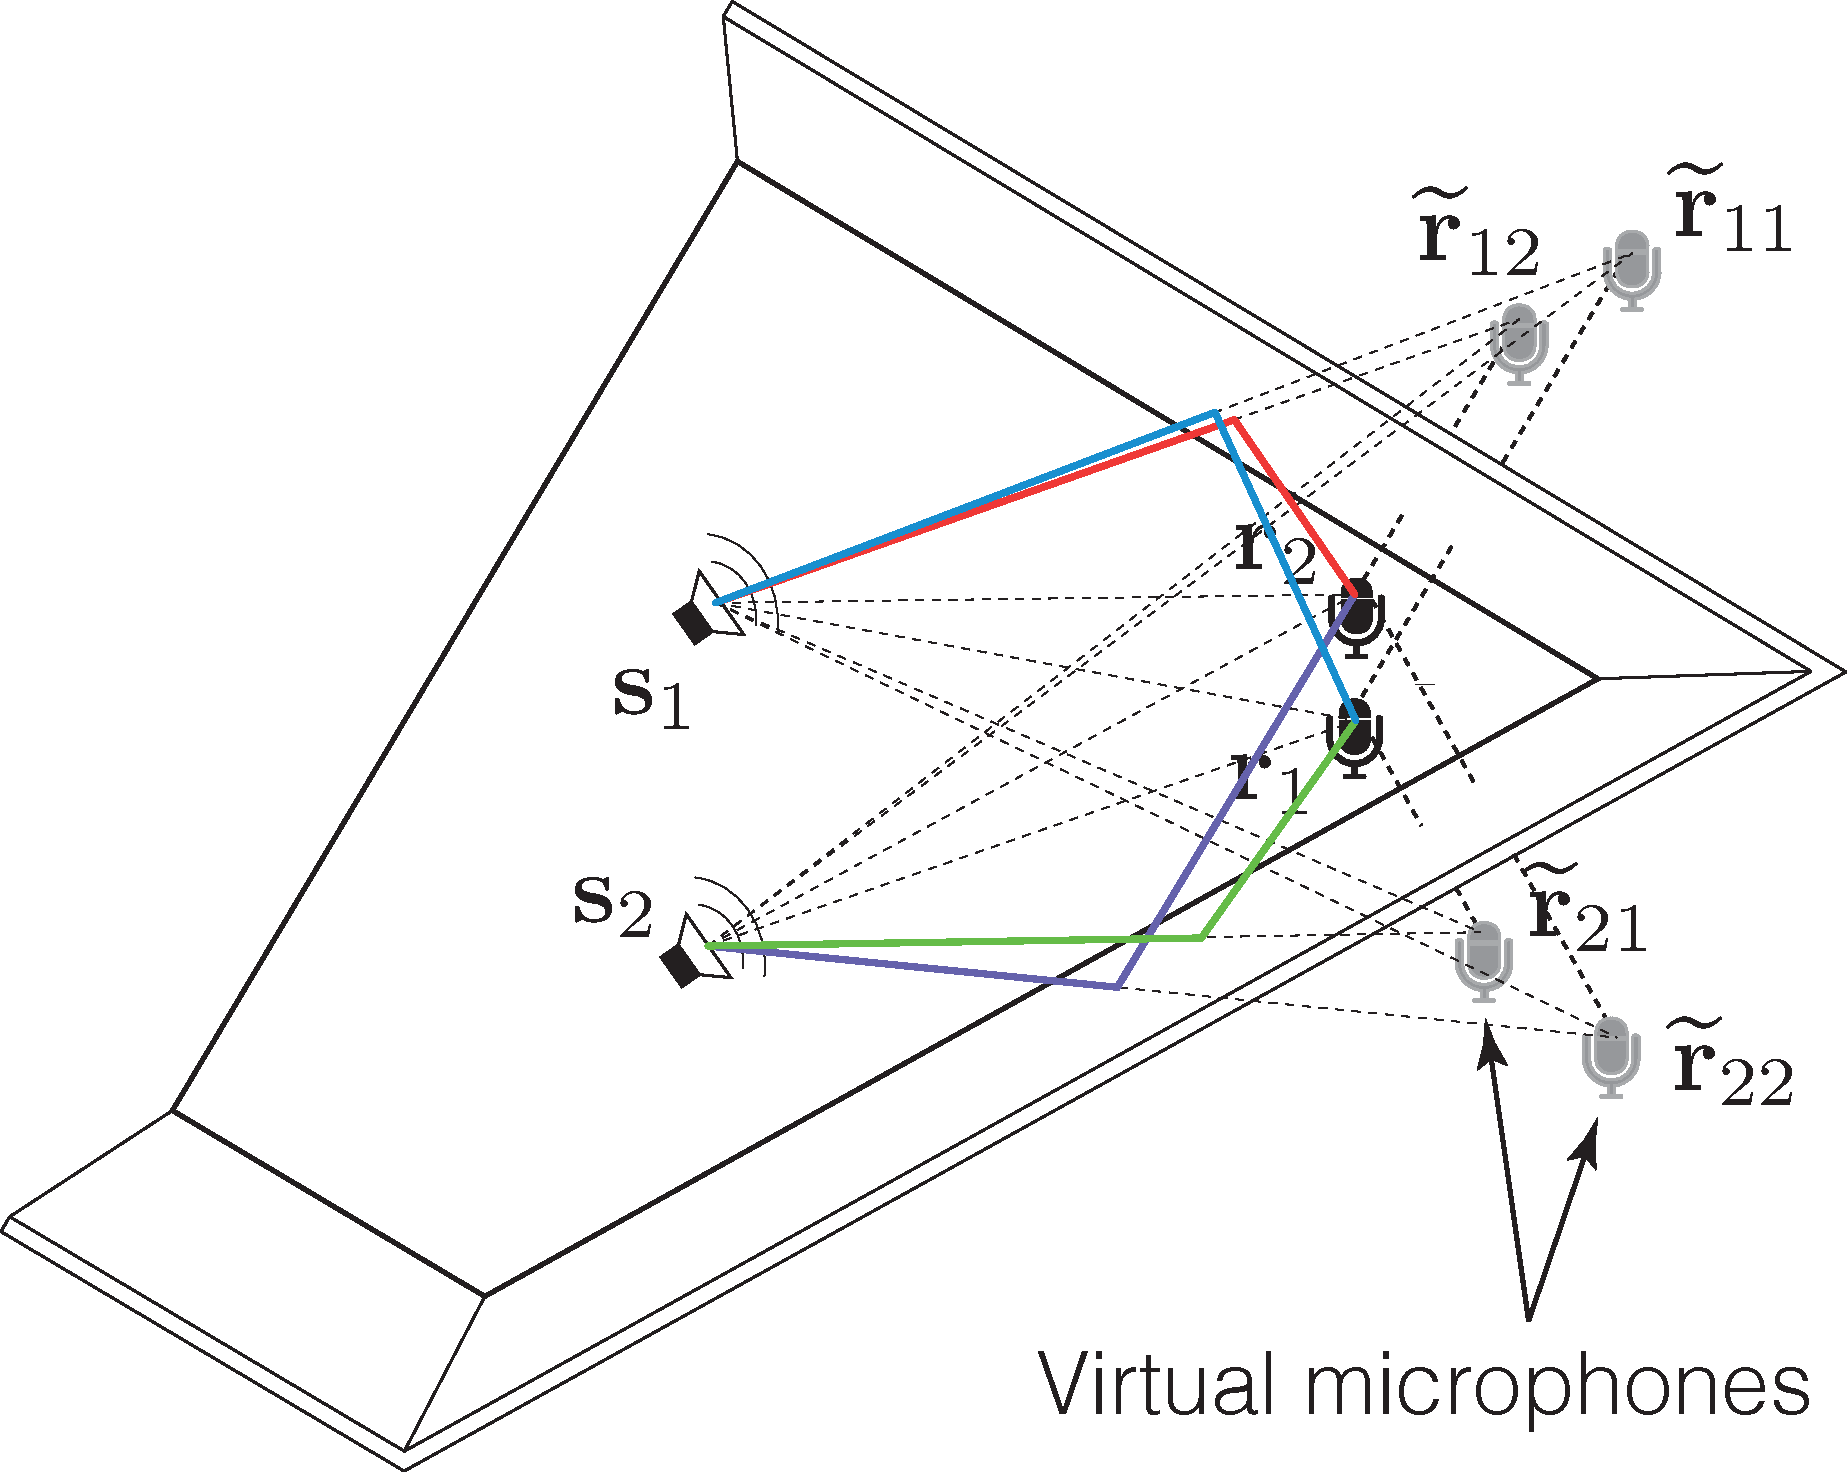
\includegraphics[width=.7\linewidth]{separake/separake.pdf}
    \caption{Typical setup with two speakers recorded by two microphones. The illustration shows the virtual microphone model (grey microphones) with direct sound path (dotted lines) and resulting first-order echoes (colored lines)}
    \label{fig:separake:setup}
    \vspace{-0mm}
\end{figure}

Real and virtual microphones form dipoles with diverse frequency-dependent directivity patterns.
Our goal is to design algorithms which benefit from this known spatial diversity.


Echoes have been used previously to enhance various audio processing tasks.
It was shown that they improve indoor beamforming \citeonly{Dokmanic:2015dr, Scheibler:2015ii, RobinThesis},
aid in sound source localization \citeonly{Ribeiro:2010uj},
and enable low-resource microphone array self-localization \citeonly{Dokmanic:2016gu}.
They have, however, rarely been analyzed in the context of source separation with non-negative source models.

\subsection{Our Goal and Main Findings}

Our emphasis here is different than that in \citeonly{leglaive2015multichannel}.
Rather than fitting the echo model, we aim to show that separation in the presence of echoes is in fact better than separation without echoes.
We ask the following questions:
\begin{enumerate}
    \item Is speech separation with echoes fundamentally easier than speech separation without echoes?
    Are there specific settings where this is true or false?
    \item Is it necessary to fully model the reverberation or can we get away with a geometric perspective where we know the locations of a few virtual microphones?
\end{enumerate}
To answer these questions we set up several simple experiments.
We take two standard, well-understood multi-channel source separation algorithms which estimate the channel (the TFs),
and instead of updating the channel estimate we simply fix it to the TFs of real and a few virtual microphones.
The first algorithm---non-negative matrix factorization (NMF) via multiplicative updates (MU)---only uses the magnitudes of the transfer functions,
while the second one---expectation maximization (EM)---also uses the phases.
In this initial investigation we look at the (over)determined case ($J \leq M$),
leaving the analysis of the undetermined case to future work. Our findings can be summarized as follows:
\begin{itemize}
    \item (MU) With magnitudes only, multi-channel anechoic separation is hardly any better than single-channel separation:
    as the magnitude of the transfer functions is the same at all microphones, channel modeling offers no diversity.
    The situation is different in rooms where the direction-dependent magnitude of TFs varies significantly from microphone to microphone.
    \textit{We show that replacing the transfer functions with a few echoes (even just one) gives significant performance gains compared to not modeling the TFs at all,
    but also that it does better than learning the TFs through multiplicative updates.}
    \item (EM) With both phases and magnitudes, anechoic separation will be near-perfect since it corresponds to a determined linear system.
    Therefore, any uncertainty from imperfections in channel modeling will make things worse.
    \textit{Surprisingly, approximating the TFs with one echo matches learning them through EM updates and using more outperforms it.}
\end{itemize}
For a sneak peak at the gains, fast forward to Figure \ref{fig:separake:results}.


\section{Modeling}

% Suppose $J$ sources emit inside the room and we have $M$ microphones.
% Each microphone receives
% \[
%     y_m(t) = \sum_{j = 1}^J c_{jm}(t),
% \]
% with $c_{jm}$ being the spatial image of the $j$th source at the $m$th microphone.
% Spatial images are given as
% \[
%     c_{mj}(t) = (x_j \conv h_{jm})(t),
% \]
% where $h_{jm}$ is the room impulse response between the source $j$ and microphone $m$.
% The room impulse response is a central object in this paper. We model it as
% \[
%     h_{jm}(t) = \sum_{k = 0}^K \alpha_{jm}^k \delta(t - t_{jm}^k) + \epsilon_{jm}(t),
% \]
% where the sum comprises the line-of-sight propagation and the earliest $K$
% echoes we want to account for (at most 6 in this paper),
% while the error term $\epsilon_{jm}(t)$ collects later echoes and the tail of the reverberation.
% We do not assume $e_{jm}(t)$ to be known.
% We assume that the sources are in the far field of real and virtual microphones so the
% times $t_{jm}^k$ depend only on the source DOAs which we assume are known.
% Assuming $K$ echoes per source are known, we can form an approximate TF from source $j$ to microphone $m$,
% \begin{equation}
%     \label{eq:separake:approx_tf}
%     \wh{H}_{j,m}(e^{j\omega}) = \sum_{k=0}^K \wh{\alpha}_{jm}^k e^{-i \omega \hat{t}_{jm}^k}.
% \end{equation}
% %The far field assumption implies that only the relative arrival times are known so we can arbitrarily fix the delay of the direct path to zero. In addition, we assume all walls to be spectrally flat and that $\alpha_{jm}^k$ are known up to a scaling (i.e. $a_{jm}^0 = 1$).
% We only assume relative arrival times and amplitudes to be known,
% that is $\hat{t}_{jm} = t_{jm}^k - t_{jm}^0$ and $\wh{\alpha}_{jm}^k = \alpha_{jm}^k / \alpha_{jm}^0$, respectively.
% In practice, these parameters can be estimated \citeonly{RemaggiThesis}.
% In addition, we assume all walls to be spectrally flat in the frequency range of interest.

% As usual, we process by frames. In the short-time Fourier transform (STFT) domain the $m$th microphone signal reads
% \begin{equation}
%     \label{eq:separake:stft_mixing}
%     Y_m[f,n] = \sum_{j = 1}^J \wh{H}_{jm}[f] X_{j}[f,n] + B_m[f,n]
% \end{equation}
% %
% with $f$ and $n$ being the frequency and frame index, $X_{j}[f,n]$ the STFT of the $j$th source signal, and $B_m[f,n]$ a term including noise and model mismatch. It is convenient to group the microphone observations in vector form,
% % Equation \eqref{eq:stft_mixing} can be written in matrix--vector form as
% \begin{equation}
%     \vY[f,n] = \wh{\mH}[f] \, \vX[f,n] + \vB[f,n].
% \end{equation}
% where $\vY[f, n] = \big[ \, Y_m[f, n] \, \big]_m$, $\wh{\mH}[f] = \big[ \, \wh{H}_{jm}[f, n] \, \big]_{m,j}$, $\vX[f, n] = \big[ \, X_j[f, n] \, \big]_j$, and $\vB[f, n] = \big[ \, B_m[f, n] \, \big]_m$.
% Let the squared magnitude of the spectrogram of the $j$th source be $\mP_j = \big[ \abs{X_{j}[f, n]}^2 \big]_{fn}$. We postulate a non-negative factor model for $\mP_j$:
% %
% \begin{equation}
%     \label{eq:nmf_model}
%     \mP_j =  \mD_j \mZ_j,
% \end{equation}
% where $\mD_j$ is the non-negative \textit{dictionary}, and the latent variables $\mZ_j$ are called \textit{activations}.
% Source separation can then be cast as an inference problem in which we maximize the likelihood of the observed $\vY$ over all possible non-negative factorizations \eqref{eq:nmf_model}. This normally involves learning the channel (frequency-domain mixing matrices). Instead of learning, we fix the channel to the earliest few echoes.

\section{Source Separation by NMF}

% To evaluate the usefulness of echoes in source separation, we modify the
% multi-channel NMF framework of Ozerov and F\'{e}votte \citeonly{ozerov2010multichannel} as follows.
% First, we introduce a dictionary learned from available training data.
% We explore both speaker-specific and universal dictionaries \citeonly{Sun:2013co}.
% Speaker-specific dictionaries can be beneficial when speakers are known in advance.
% Universal dictionary is more versatile but gives a weaker regularization prior.
% Second, rather than learning the TF from the data, we use the approximate model of \eqref{eq:approx_tf}.
% In the following we briefly describe the two algorithms used.

\subsection{NMF using Multiplicative Updates (MU-NMF)}\label{sec:mu}

% Multiplicative updates for NMF only involve the magnitudes and are simpler than the EM updates.
% The updates are guaranteed non-negative as long as the intitialization is.
% They have been originally proposed by Lee and Seung \citeonly{Lee:2001ti}.
% We use the Itakura-Saito divergence \citeonly{Fevotte:2011af} between the observed multi-channel squared magnitude spectra $\mV_m = [|Y_m[f,n]|^2]_{fn}$ and their non-negative factorizations,
% \begin{equation}
%     \label{eq:mu_nmf_model}
%     \wh{\mV}_m = \sum_{j=1}^{J} \diag(\vQ_{jm}) \mD_j \mZ_j, \quad m=1,\ldots,M
% \end{equation}
% where $\vQ_{jm} = \big[ \, |\wh{H}_{jm}[f]|^2 \,\big]_f$ is the vector of squared magnitudes of the approximate TF between microphone $m$ and source $j$.
% We add an $\ell_1$-penalty term to promote sparsity in the activations due to the potentially large size of the universal dictionary~\citeonly{Sun:2013co}.
% The cost function is thus
% \begin{equation}
%     C_{\mathsf{MU}}(\mZ_j) = \sum_{mfn} d_{\mathsf{IS}}(V_{m}[f,n] | \wh{V}_{m}[f,n])
%     + \gamma \sum_j \| \mZ_j \|_1,
% \end{equation}
% where $d_{\mathsf{IS}}(v | \hat{v}) = \frac{v}{\hat{v}} - \log \frac{v}{\hat{v}} - 1$.
% By adapting the original MU rule derivations from Ozerov and F\'{e}votte, we obtain the following regularized MU update rule:
% \begin{align}
%     \mZ_j \gets \mZ_j \odot \frac{\sum_m (\diag(\vQ_{ij}) \mD_j)^\top \left(\mV_j \odot \wh{\mV}_j^{-2}\right)}{\sum_m(\diag(\vQ_{ij}) \mD_j)^\top \wh{\mV}_j^{-1} + \gamma},
% \end{align}
% where multiplication $\odot$, power, and division are element-wise.

% Importantly, neglecting the reverberation (or working in the anechoic regime) leads to a constant $\vQ_{jm}$ for all $j$ and $m$. A consequence is that the MU-NMF framework breaks down with a universal dictionary. Indeed, \eqref{eq:mu_nmf_model} becomes the same for all $m$,
% $
%     \wh{\mV}_m = \sum_{j} \mD \mZ_j = \mD \sum_j \mZ_j,
% $
% so even with the correct atoms identified, we can assign them to any source without changing
% the value of the cost function. Therefore, anechoic multi-channel separation with a universal dictionary cannot work well. This intuitive reasoning is corroborated by numerical experiments in Section \ref{sec:results}.
% %The problem is overcome by the EM-NMF algorithm which keeps the channel phase and is thus able to exploit the phase diversity across the array. Of course, in line with the message of this paper, it is also overcome by using echoes.
% Of course, in line with the message of this paper, this problem is overcome by using echoes.

\subsection{NMF using Expectation Maximization (EM-NMF)}

% Unlike the MU algorithm that independently maximizes the log-likelihood of TF magnitudes, EM-NMF maximizes the joint log-likelihood over all complex-valued channels~\citeonly{ozerov2010multichannel}. Hence, it takes into account observed phases.
% Each source $j$ is modeled as the sum of components with complex Gaussian priors of the form $c_{k}[f,n]\sim \mathcal{C}\mathcal{N}\Big(0, d_{fk}z_{kn}\Big)$ such that
% \begin{equation}
%     X_j[f,n] \sim \mathcal{C}\mathcal{N}\left(0, (\mD_j\mZ_j)_{fn}\right),
% \end{equation}
% and the magnitude spectrum $\mP_j$ of \eqref{eq:nmf_model} can be understood as the variance of source $j$.
% Under this model, and assuming uncorrelated noise, the microphone signals also
% follow a complex Gaussian distribution with covariance matrix
% \begin{equation}
%     \mSigma_{\vY}[f,n] = \wh{\mH}[f] \, \mSigma_\vX[f,n] \, \wh{\mH}^H[f] + \mSigma_\vB[f,n],
% \end{equation}
% and the negative log-likelihood of the observed signal is
% \begin{equation}\nonumber %label{eq:EMcriterion}
% \resizebox{\linewidth}{!}{
%     $C_{\mathsf{EM}}(\mZ_j) = \sum\limits_{fn} \trace\left(\vY[f,n]\vY[f,n]^H\mSigma_{\vY}^{-1}[f,n]\right) \\
%     + \log\det\mSigma_{\vY}[f,n].$
%     }
% \end{equation}
% This quantity can be efficiently minimized using the EM algorithm proposed in~\citeonly{ozerov2010multichannel}. We modify the original algorithm by fixing the source dictionaries $\mD_j$ and the early-echo channel model $\wh{\mH}[f]$ throughout the iterations.
% Since adding sparsity priors is not straightforward in the EM framework, the universal dictionary was left for future work.

\section{Numerical Experiments}

% We test our hypotheses through computer simulations. In the following, we describe the simulation setup, dictionary learning protocols, and we discuss the results.

\subsection{Setup}

% An array of three microphones arranged on the corners of an equilateral triangle with edge length 0.3~m is placed in the corner of a 3D room with 7 walls. We select 40 sources at random locations at a distance ranging from 2.5~m to 4~m from the microphone array. Pairs of sources are chosen so that they are at least 1~m apart. The floor plan and the locations of microphones are depicted in Figure~\ref{fig:rir_room}. The scenario is repeated for every two active sources out of the 780 possible pairs.

% \begin{figure}
%     \centering
%     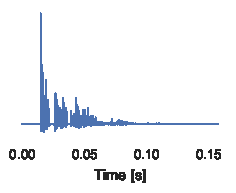
\includegraphics{figures/typical_rir}
%     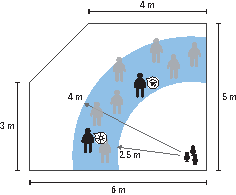
\includegraphics{figures/room_setup}
%     \caption{Left, a typical simulated RIR. Right, the simulated scenario.}
%     \label{fig:rir_room}
% \end{figure}

% The sound propagation between sources and microphones is simulated using the
% image source model implemented in \textit{pyroomacoustics} Python package~\citeonly{scheibler2017pyroomacoustics}. The wall absorption factor is set to 0.4, leading to a T60 of approximately 100~ms. An example RIR is shown in Figure~\ref{fig:rir_room}. The sampling frequency is set to 16~kHz, STFT frame size to 2048 samples with 50\% overlap between frames, and we use a cosine window for analysis and synthesis. Partial TFs are then built from the $K$ nearest image microphones. The global delay is discarded. %, and only the relative amplitudes between echoes are kept.

%\textcolor{red}{TODO: mention that the wall absorption is assumed known throughout experiments. What about the absorption of walls which are further from the array? Is it the same for all walls?}

% With this setup, we perform three different experiments. In the first one, we evaluate MU-NMF with a universal dictionary. In the other two, we evaluate the performance of MU-NMF and EM-NMF with Speaker-specific dictionaries. We vary $K$ from 1 to 6 and use three baseline scenarios:
% \begin{enumerate}
% \item \textit{anechoic}: Anechoic conditions, no model mismatch.
% \item \textit{learn}: The TFs are learned from the data along the activations as originally proposed~\citeonly{ozerov2010multichannel}.
% \item \textit{no echoes}: Reverberation is present but ignored (i.e. $K=0$).
% \end{enumerate}
% With the universal dictionary, the large number of latent variables warrants the introduction of sparsity-inducing regularization. The value of the regularization parameter $\gamma$ was chosen by a grid search on a holdout set with the signal-to-distortion ratio (SDR) as the figure of merit \citeonly{vincent2007first} (Table~\ref{tab:gamma}).

% \begin{table}
%     \centering
%     \begin{tabular*}{\linewidth}{@{\extracolsep{\fill}}lccccccccc@{}}
%         \toprule
%          &       &          & \multicolumn{7}{c}{{\footnotesize Number of echoes $K$}} \\
%          \cmidrule{4-10}
%          & anechoic & learn & 0 & 1 & 2 & 3 & 4 & 5 & 6 \\
%          \cmidrule{2-10}
%          $\gamma = $ & $10$ & $10^{-1}$ & $10$ & $10^{-3}$ & 0 & 0 & 0 & 0 & 0 \\
%          \bottomrule
%     \end{tabular*}
%     \caption{Value of the regularization parameter $\gamma$ used with the universal dictionary.}
%     \label{tab:gamma}
%     \vspace{-0mm}
% \end{table}


% \begin{figure*}
%     \centering
%     \subfloat[mu_univ][MU-NMF, Universal dictionary]{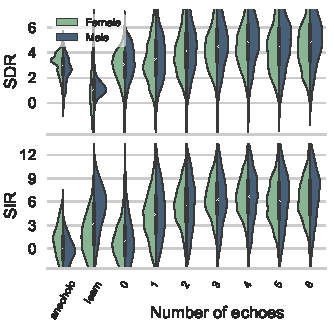
\includegraphics{figures/20171025-111558_5ae4058906_near_wall_mu_UnivDict_violin_plot.pdf}\label{fig:mu_univ}}
%     \hfill
%     \subfloat[mu_spkr][MU-NMF, Speaker-specific dictionary]{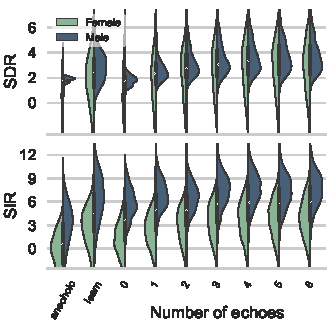
\includegraphics{figures/20171026-192746_360771b8ce_near_wall_mu_SpkrDict_violin_plot.pdf}\label{fig:mu_spkr}}
%     \hfill
%     \subfloat[em_spkr][EM-NMF, Speaker-specific dictionary]{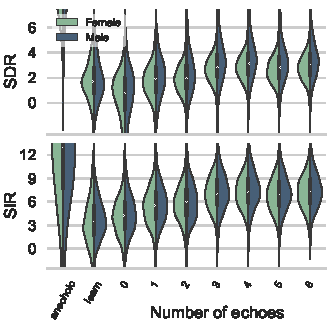
\includegraphics{figures/20171027-050909_e9d8c07aef6_near_wall_em_SpkrDict_violin_plot.pdf}\label{fig:em_spkr}}
%     \caption{Distribution of SDR and SIR for male and female speakers as a function of the number of echoes included in modeling, and comparison with the three baselines.}
%     \label{fig:results}
%     \vspace{-0mm}
% \end{figure*}

% \begin{figure}
%     \centering
%     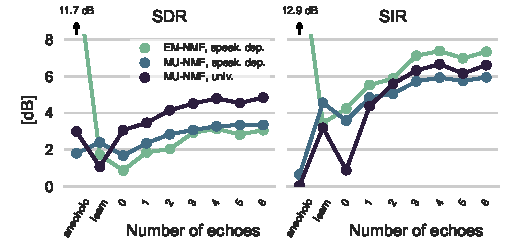
\includegraphics{figures/all_medians.pdf}
%     \caption{Summary of the median SDR and SIR for the different algorithms evaluated.\vspace{-3mm}}
%     \label{fig:median}
% \end{figure}

% \subsection{Dictionary Training, Test Set, and Implementation}


% \textit{Universal Dictionary:} Following the methodology of \citeonly{Sun:2013co} we select 25 male and 25 female speakers
% and use all available training sentences to form the universal dictionary
% $
%     \mD = [\mD_1^\mathsf{M}\cdots \mD_{25}^\mathsf{M} \, \mD_{1}^\mathsf{F}\cdots\mD_{25}^\mathsf{F}].
% $
% The test signals were selected from speakers \emph{and} utterances outside the training set.
% The number of latent variables per speaker is 10 so that with STFT frame size of 2048 we have $\mD\in\R^{1025\times500}$.

% \textit{Speaker-Specific Dictionary:}  Two dictionaries were trained on one male and one female speaker. One utterance per speaker was excluded to be used for testing. The number of latent variables per speaker was set to 20.

% All dictionaries were trained on samples from the TIMIT corpus \citeonly{garofolo1993timit} using the NMF solver in \textit{scikit-learn} Python package~\citeonly{pedregosa2011scikit}.

% \textit{Implementation:} Authors of \citeonly{ozerov2010multichannel} provide a Matlab implementation of MU-NMF and EM-NMF methods for stereo separation. We ported their code to Python and extended it to arbitrary number of input channels.\footnote{Our implementation and all experimental code are publicly available in line with the philosophy of reproducible research.} The number of iterations for MU-NMF (EM-NMF) was set to 200 (300) and simulated annealing in EM-NMF implementation was disabled.
% %However this software features some ad-hoc decisions which do not fit our scenario. Thus, we provide a Python3 adaptation with the following modifications.
% %\\First the original code was restricted to the 2-channel case, i.e.  $M = 2$.  Thus, in order to embrace the specifics of our scenario and for sake of generalization, we extend it to the multi-channel case, that is $\forall M > 1$.
% %\\Secondly, the MU-NMF was modified to handle sparsity contraint as described in \ref{sec:mu}.
% %\\Third, since EM method degenerates where zero-valued entries are present in the dictionary matrix, $\mD$, all these entries are initially set to a small constant value of \texttt{1e-6}.
% %\\Finally, the code was further modified to deal with fixed dictionary and channel models matrices, which are normalized in order to avoid indeterminacy issues \citeonly{ozerov2010multichannel}.
% %\\Now to conclude with, no \textit{simulated annealing} strategies are not used in the final experiments. In fact in some preliminary and informal investigations we noticed that this yields to better results then using annealing. In the experiments, the number of iterations was set to $300$.

\subsection{Results}
\label{sec:results}

% We evaluate the performance in terms of signal-to-distortion ratio (SDR) and source-to-interference ratio (SIR) as
% defined in \citeonly{vincent2007first}. We compute these metrics using the \textit{mir\_eval} toolbox~\citeonly{raffel2014mir_eval}.

% The distributions of SDR and SIR for separation using MU-NMF and a universal dictionary are shown in Figure~\ref{fig:mu_univ}, with a summary in Figure~\ref{fig:median}. We use the median performance to compare the results
% from different algorithms.
% First, we confirm that separation fails for flat TFs (\textit{anechoic} and $K=0$) with SIR at around 0~dB. Learning the TFs performs somewhat better in terms of SIR than in terms of SDR, though both are low. Introducing approximate TFs dramatically improves performance: the proposed approach outperforms the learned approach even with a single echo. With up to six echoes, gains are +2~dB SDR and +5~dB SIR. Interestingly, with more than one echo, $\ell_1$ regularization becomes unnecessary; non-negativity and echo priors are sufficient for separation.

% Separation with speaker-dependent dictionaries is less challenging since we have a stronger prior. Accordingly, as shown in Figures~\ref{fig:mu_spkr} and \ref{fig:median}, MU-NMF now achieves a certain degree of separation even without the channel information. The gains from using echoes are smaller, though one echo is still sufficient to match the median performance of learned TFs. Using an echo, however, results in a smaller variance. Adding more echoes further improves SDR (SIR) by up to +2~dB (+3~dB).

% In the same scenario, EM-NMF (Figure~\ref{fig:em_spkr}) has near-perfect performance on anechoic signals which is expected as the problem is overdetermined. For MU, a single echo suffices to reach the performance of learned TFs and further improve it. Moreover, echoes
% significantly improve separation quality as
% illustrated by up to 3~dB improvement over \textit{learn}. It is interesting to note that in all experiments the first three echoes near-saturate the metrics. This is good news since higher order echoes are hard to estimate.

%\begin{itemize}
%    \item Universal dictionary scenario: Here, the speakers are unknown.
%    \begin{itemize}
%        \item Because the MU method does not use phase and hence no time delay information across channels, source separation in the anechoic scenario is impossible. Here, we see that using reverberated signals instead with knowledge of only a few echoes significantly improve source separation performance: up to +2dB SDR and +5 dB SIR.
%        \item Using a fixed echo model for channels also outperform learning the channels, even with a single echo.
%        \item Note that EM could not be used for the universal dictionary scenario, because the corresponding model is not designed to handle dictionaries with hundreds of atoms. A sparsity-enforcing Bayesian prior on the estimated activation Z would need to be included, which is not straightforward.
%        \item Increasing the number of known echoes beyond 3 does not bring significant improvement.
%    \end{itemize}
%    \item Speaker-dependent dictionary scenario. This scenario is on the one hand easier because speakers are known and on the other hand harder because much less training data is used, allowing much fewer atoms to represent speech in the dictionaries.
%    \begin{itemize}
%        \item Unsurprisingly, EM performs extremely well in the anechoic setting. This is because perfect knowledge of the complex-valued over-determined mixing filters is then available, through the time differences of arrival. Results would likely be very different in an under-determined setting, where perfect filter knowledge is not enough to separate signals.
%        \item Once again, it is showed that using knowledge of a few echoes significantly improve results with respect to an anechoic model, up to +2dB SDR and +3dB SIR for both methods.
%        \item EM performs slightly better (+1.5 dB) than MU in terms of SIR, suggesting that modeling the phase of mixing filters help.
%        \item In this scenario, knowledge of the echoes starts significantly outperforming the baseline (the learned model) when 3 echoes are known (+3dB SIR).
%        \item Again, increasing the number of known echoes beyond 3 does not bring significant improvement.
%    \end{itemize}
%\end{itemize}

\section{Conclusion}

% In this paper we began studying the role of early echoes in sound source separation---a challenging task in computational auditory scene analysis. We found that a simple echo model not only improves performance, but it also enables separation in conditions where it is otherwise not possible. One such example is separation with non-negative speaker-independent models. Echoes seem to play an essential role in magnitude-only algorithms like non-negative matrix factorization via multiplicative updates. They improve separation as measured by the standard metrics even when compared to approaches that learn the transfer functions. We believe these results are only a first step in understanding the potential of echoes in computational auditory scene analysis. They suggest that simple models used in this paper could be used as regularizers in other common audio processing tasks. Ongoing work includes running real experiments, studying the underdetermined case, and blindly estimating the wall parameters.

%Future work:
%\begin{itemize}
%    \item Update the late-reverberation part of mixing matrices in EM
%    \item Adding sparsity priors to activations to use larger dictonary with EM
%    \item Experiments with more microphone/room configurations, more sources
%    \item Use a DOA estimation algorithm to infer the early echo models.
%    \item Estimate the absorption factors of nearby surfaces.
%\end{itemize}

%Echoes are our friends! They really are!
% \chapter{\mirage: Sound Source Localization with Echoes}\label{chap:mirage}

\marginpar{%
\footnotesize
Sound Source Localization, Image Microphones, TDOA Estimation, Supervised Learning.
}
\newthought{Synopsis} It is commonly observed that acoustic echoes hurt performance of sound source localization (SSL) methods.
We introduce the concept of microphone array augmentation with echoes (MIRAGE) and
show how estimation of early-echo characteristics can in fact benefit SSL.
We propose a learning-based scheme for echo estimation combined with a physics-based scheme for echo aggregation.
In a simple scenario involving 2 microphones close to a reflective surface and one source,
we show using simulated data that the proposed approach performs similarly
to a correlation-based method in azimuth estimation while retrieving
elevation as well from 2 microphones only, an impossible task in anechoic settings.

\section{Introduction}

% \subsection{Literature review: an acoustic perspective}
% Bibliography with respect to sound propagation

% \subsection{Literature review an algorithmic perspective}
% Bibliography with respect to learning and knowledge approaches

% \newthoughtpar{Knowledge-based vs. learning-based approaches}

% \newthoughtpar{Regression vs. classification approaches}

% \section{Background in SSL}
% \begin{itemize}
%     \item 1D SSL: AOA estimation
%     \item 2D SSL: azimuth and elevation estimation
%     \item 3D SSL: polar and cartesian coordinates
% \end{itemize}

% \subsection{Stereophonic SSL and 1D SSL}

% \newthoughtpar{Binaural SSL}

% \subsection{Multichannel SSL and 2D SSL}

% \section{\mirage: microphone augmentation with echoes}

% \section{Experimental evaluation}

% --- Margin Figure
\marginpar{%
    \centering
    \footnotesize
    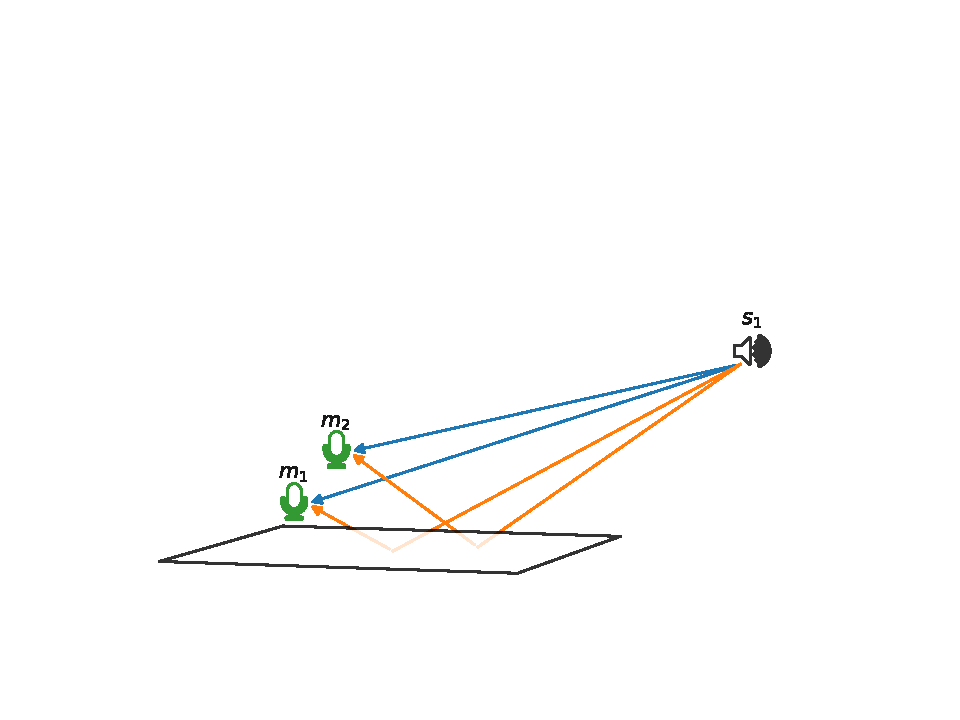
\includegraphics[trim={50 70 50 150},clip,width=\linewidth]{mirage/scene.pdf}
    \captionof{figure}{%
        Typical setup with one source source recorded by two microphones.
        The illustration shows direct sound path (blue lines) and resulting first-order echoes (orange lines).}
    \label{fig:mirage:scene}
}
Sound source localization (SSL) consists in determining the position of a sound source from microphone signals in 3D space.
In polar coordinates, most existing methods focus on estimating the directional of arrival, namely, azimuth and elevation angles.
Though this task is performed routinely by humans, it still challenges today's computational methods,
in particular in the presence of reverberation or interfering sources (see \cite{rascon2017localization} and \cite{Argentieri2015} for a review).
Computational approaches consist in two components. First, extracting features from audio data that are as independent
as possible from the source's content while preserving spatial information. Second, mapping these features to the source position.
Two lines of research have been investigated to obtain such mappings: physics-based and learning-based approaches.

\newthought{Physics-based approaches} rely on a simplified sound propagation model
\cite{rascon2017localization,Knapp1976,DiBiase2001,Lebarbenchon2018}.
The free-field model is by far the most widely used one and assumes
a single direct sound path from the source to each microphone.
When the source is placed far enough, this yields a closed-form mapping from the
sound's time-difference-of-arrival (TDOA) in a microphone pair and the source's azimuth angle in this pair.
If multiple microphone pairs are available and form a non-linear array,
their TDOAs can be aggregated to obtain 2D directions of arrival \cite{DiBiase2001}.
These methods strongly suffer in environments where the free-field assumption is violated,
\textit{e.g.}, in the presence of strong acoustic echoes and reverberation \cite{Scheuing2006}.

\newthought{Learning-based approaches} use an annotated training dataset to implicitly
learn a mapping from audio features to source positions
\cite{deleforge2015acoustic, Vesperini2016, Adavanne2017,  Perotin2018, gaultier2017vast}.
Such data can be obtained from real recordings \cite{deleforge2015acoustic} or
using physics-based simulators \cite{Vesperini2016, Adavanne2017,  Perotin2018, gaultier2017vast}.
These methods were showed to overcome some limitations of the free-field model,
but are usually trained for specific microphone arrays and fail whenever test conditions strongly mismatch training conditions.

Most sound source localization methods, including the above listed,
regard reverberation and in particular acoustic echoes as a nuisance.
In contrast, some recent work that we refer to as \textit{echo-aware}
methods have showed that the knowledge of early acoustic echoes could
be used to reconstruct the geometry of an audio scene \cite{Nakashima2010,dokmanic2013acoustic,An2018}
or to improve performance of signal enhancement methods \cite{flanagan1993spatially, dokmanic2015raking,Scheibler2017}.
In \cite{Nakashima2010}, some ad-hoc reflectors are used as artificial \textit{pinnae}
to estimate elevation based on a simple reflection model.
In \cite{An2018}, cameras, depth sensors and laser sensors are used to
identify reflectors and build a corresponding acoustic model that helps SSL.

\newthought{In this work,} we combine ideas from physics-based, learning-based and echo-aware approaches
to introduce the framework of \underline{mi}crophone a\underline{r}ray
\underline{a}u\underline{g}mentation with \underline{e}choes (MIRAGE) for SSL.
We consider a simple yet common scenario to illustrate this idea:
two microphones, one source and a nearby reflective surface, as illustrated in Fig. \cref{fig:scene}.
This may occur, for instance, when the sensors are placed on a table such as in
voice-based assistant devices or next to a wall.
The reflective surface is assumed to be the most reflective and closest one to the microphones in the environment,
hence generating the strongest and earliest echo in each microphone.
Under this \textit{close-surface} model, we ask the following questions:
\begin{enumerate}
\setlength\itemsep{-1mm}
\item Can early echoes be estimated from two-microphone recordings of an unknown source?
\item Can they be used to estimate both the azimuth and elevation angles of the source, an \textit{impossible} task in free field conditions?
\end{enumerate}
We propose to use a deep neural network (DNN) trained on a simulated close-surface dataset to estimate early echoes properties from audio features.
The MIRAGE framework then exploits these estimated properties by expressing them as TDOAs in the \textit{virtual 4-microphone array}
formed by the true microphone pair and its image with respect to the reflective surface.
We show that the proposed framework approximately estimates echo properties,
perform similarly to a correlation-based method in azimuth estimation for the considered
scenario and estimates \textit{impossible} elevation angles with good accuracy in noiseless settings using two microphones only.

\section{Background in microphone array SSL}\label{sec:background}
In this section, we briefly review some necessary background in microphone array SSL. Let us assume a microphone array of $I$ sensors is placed inside a room and records the sound emitted by one static point sound source. In all generality, the relationship between the signal $m_i(t)$ recorded by the sensor placed at fixed position $\mathbf{m}_i$ and the signal $s(t)$ emitted by the source at fixed position $\mathbf{s}$ is defined by:
\begin{equation}\label{eq:mirage:anymic_time}
m_i(t) = (h_i * s)(t)  \; + \; n_i(t),
\end{equation}
where the convolution with room impulse response (RIR) $h_i(t)$ embodies the fact that sensor $i$ receives a so-called spatial image of the source and $n_i$ denotes possible measurement noise. The RIR depends on the spatial parameters of the scene: microphone positions, source position w.r.t the room, as well as the room acoustic properties (size, absorption and diffuseness of the wall materials.)

RIRs can be typically modelled as the sum of the direct path and multiple reflections of the sound. This can boil down to modelling $h_i$ as a Dirac impulse at time $\tau_i$ accounting for the time delay from the source to microphone $i$, plus an error term. In the frequency domain, this leads to:
\begin{equation}\label{eq:mirage:rir}
H_i(f) = \alpha_i(f) \; e^{- 2 \pi f \tau_i} \; + \; \varepsilon_i(f),
\end{equation}
where the error term $\varepsilon_i(t)$ collects echoes, the reverberation tail, diffusion, and noise. The term $\alpha_i(f)$ captures the air attenuation phenomenon. A time-domain example of RIR is shown in Fig.~\cref{fig:rirs} (left).

% --- In text figure with caption on the margin (side)
\begin{figure}[t]
    \begin{sidecaption}[RIRs within the MIRAGE framework]{%
        Left, a typical simulated RIR with annotated components. Right, superposition of two RIRs and visualization of time difference
        of arrival between direct paths (TDOA), first echoes (iTDOA) and direct path and first echo (TDOE).
    }[fig:mirage:rirs]
    \centering
    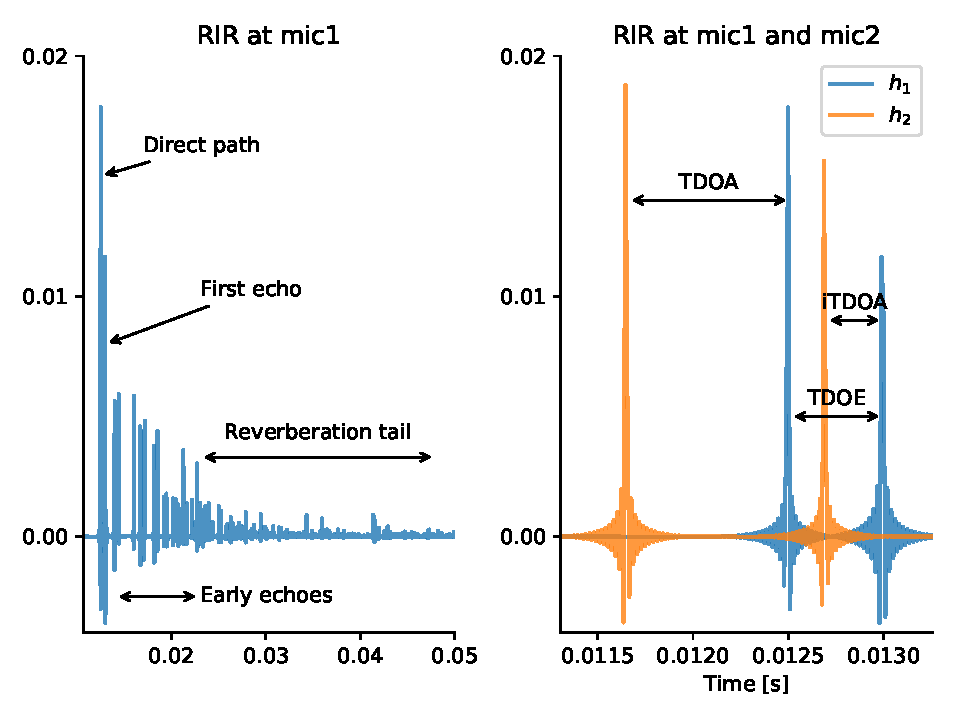
\includegraphics[trim={0 5 0 0},clip,width=\linewidth, height=0.6\linewidth]{mirage/rirs.pdf}
    \end{sidecaption}
\end{figure}


\subsection{2-channel 1D-SSL}\label{subsec:mirage:1D-SSL}
Let us first consider the stereo case ($I=2$). Under the far-field assumption,
traditional SSL methods use the time difference of arrival (TDOA),
$\tau \triangleq \tau_2 - \tau_1$, as a proxy for the estimation of the angle of arrival (AOA), since:
\begin{equation}\label{eq:mirage:aoa}
\text{AOA} = \text{arccos} \left(c \: \tau \: / \:d \right),
\end{equation}
where $c$ is the speed of sound and $d$ the inter-microphone distance.
SSL then reduces to estimating the TDOA, which can be done by cross-correlation-based methods such as
the widely used and well performing generalized cross-correlation
with phase transform (GCC-PHAT) method \cite{Knapp1976,Blandin2012}.
Given short-time Fourier transforms $M_1$ and $M_2$ of the two microphones signals,
the GCC-PHAT \textit{angular spectrum} is defined as:
\begin{equation}\label{eq:mirage:gccphatcontrast}
\Psi_\text{GCC}(\tau) = \sum_{f,n}\frac{M_1(f,n) M_2^*(f,n)}{\mid M_1(f,n) M_2^*(f,n) \mid} e^{-2\pi f \tau}.
\end{equation}
Then, the TDOA estimate is given by $\hat{\tau} = \arg \underset{\tau}{\max} \; \Psi_\text{GCC}(\tau)$.
Note that $\Psi_\text{GCC}$ can also be expressed directly as a function of the
AOA using \eqref{eq:mirage:aoa}, hence the term \textit{angular spectrum}.
This method was showed to be state-of-the-art in a large benchmark \cite{Blandin2012}.

\subsection{Multichannel 2D-SSL}\label{subsec:mirage:2D-SSL}
When more microphones are available and the array is not linear, 2D-SSL can be envisioned.
A possible approach is to use 1D-SSL on all pairs and combine their results,
a principle which was successfully applied in the steered response power with phase transform (SRP-PHAT) method \cite{DiBiase2001}.
SRP-PHAT exploits the geometry of the microphone array and the estimated TDOAs from microphone pairs to return the DOA.
In a nutshell, this algorithm aims to estimate a global angular spectrum $\Psi_{\text{SRP}}(\theta,\phi)$
which will exhibit a local maximum in the direction of the active source.
First, a global grid of possible DOAs is defined according to a desired resolution and computational load.
Second, for each pair of microphones, a local set of AOAs is defined and a TDOA-based algorithm (e.g. GCC-PHAT)
is used to compute the associated local angular spectrum.
Finally all the local contributions (a collection of local $\Psi_\text{GCC}(\tau)$) are geometrical
aggregated and interpolated back to the global DOA grid to form $\Psi_{\text{SRP}}(\theta,\phi)$,
and the DOA maximizing $\Psi$ is used as estimate.
\marginpar{%
\centering
\footnotesize
    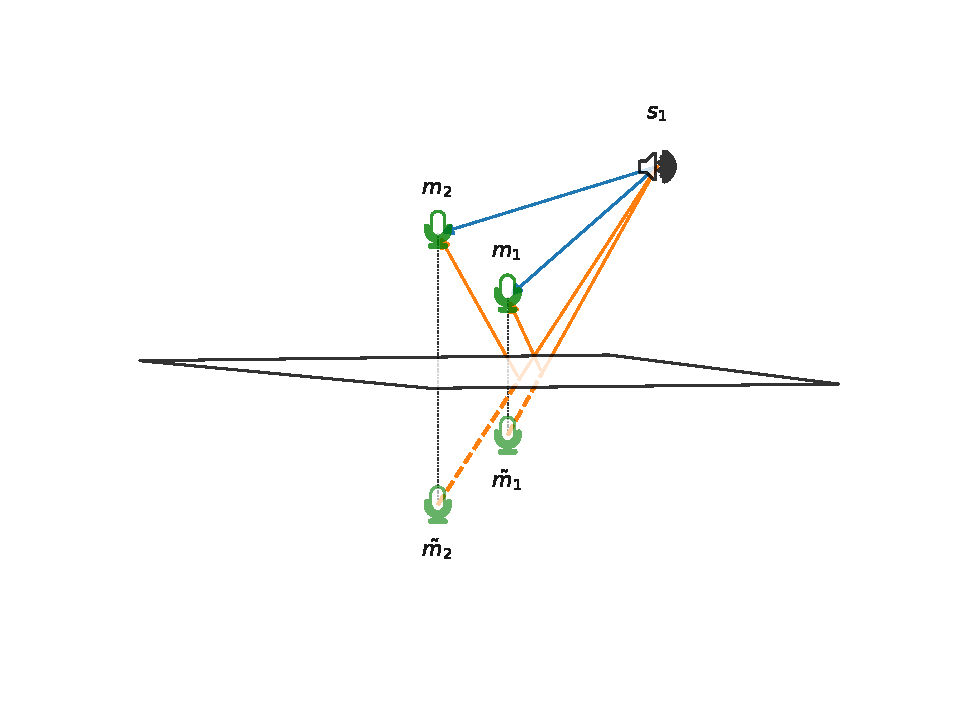
\includegraphics[trim={90 75 40 50},clip,width=\linewidth]{mirage/mirage.pdf}
    \captionof{figure}{%
        Illustration of the images $\tilde{m}_1$ and $\tilde{m}_2$ of microphones $m_1$ and $m_2$ in the presence of a reflective surface and a source.
        Blue lines correspond to direct paths, orange lines correspond to echo paths.}
    \label{fig:mirage:mirage}
}


\section{MIRAGE: Microphone Array Augmentation with Echoes}\label{sec:mirage:mirage}
We now introduce the proposed concept of \underline{mi}crophone a\underline{r}ray
\underline{a}u\underline{g}mentation with \underline{e}choes (MIRAGE).
Let us first expand formula~\eqref{eq:mirage:rir} to account for more echoes:
\begin{equation}
\label{eq:mirage:echo_h}
H_i(f) = \sum_{k=0}^{K}\alpha_i^k(f) \; e^{- 2 \pi f \tau_i^k} \; + \; \varepsilon_i(f)
\end{equation}
where the sum now comprises the direct path ($k=0$) and the $K$ earliest reflections ($K = 1$ in this paper)
and $\varepsilon_i$ collects the remaining RIR components.
Here, $\alpha_i^k(f)$ accounts for both air attenuation and wall absorption phenomena.
In the remainder of this paper, we make the approximation of frequency-independent $\alpha_i^k$.
Eq.~\cref{eq:mirage:echo_h} then corresponds to the well known image-source (IS) model,
where reflections are treated as mirror images of the true source with respect to reflective surfaces,
emitting the same signal.
We will employ here a less common but equivalent interpretation of IS,
namely, the image-microphone (IM) model. As illustrated in Fig.~\cref{fig:mirage:mirage},
virtual microphones are mirror images of the true microphones with respect to reflective surfaces.
In this view, the echoic signal received at a true microphone
is the sum of the anechoic signals received at this microphone and its images.
If we consider the virtual array consisting of both true and image microphones,
multiple microphone pairs are now available. For each of them,
it is then possible to define a corresponding time difference of arrival.
Among them, we will refer to the one between the two real microphones as TDOA,
the one between the two image microphones as image TDOA (iTDOA) and the one between
the first microphone and its image as time difference of echoes (TDOE).
We have:

\begin{align}
\text{TDOA} &= (\norm{\mathbf{m}_2 - \mathbf{s}}
                - \norm{\mathbf{m}_1 - \mathbf{s}})/c
                = \tau_2^0 - \tau_1^0,\\
\text{iTDOA}&= (\norm{\tilde{\mathbf{m}}_2 - \mathbf{s}}
                - \norm{\tilde{\mathbf{m}}_1 - \mathbf{s}})/c
                = \tau_2^1 - \tau_1^1,\\
\text{TDOE} &= (\norm{\tilde{\mathbf{m}}_1 - \mathbf{s}}
                - \norm{\mathbf{m}_1 - \mathbf{s}})/c
                = \tau_1^1 - \tau_1^0,
\end{align}

where $\tilde{\mathbf{m}}_i$ denotes the image of position $\mathbf{m}_i$.
These three quantities are directly connected to RIRs, as illustrated in Fig.~\cref{fig:mirage:rirs}(right).
Let $V = \{ \text{TDOA}, \text{iTDOA}, \text{TDOE}\}\in\mathbb{R}^3$.
Following the 2D-SSL scheme described in Sec. \cref{subsec:mirage:2D-SSL} and
given the virtual microphone-array geometry (which depends on the relative position of microphones to the surface),
$V$ could in principle be used to estimate the 2D directional of arrival of the source.
In the next section, we present a learning-based method to estimate
$V$ using audio features obtained from only two microphones.

\section{Learning-based echo estimation}
Our approach is to train a deep neural network (DNN) on a dataset simulating the considered close-surface scenario.
We model the problem as multi-target regression, with \textit{interaural level difference} (ILD)
and \textit{interaural phase difference} (IPD) as input features, and $V \in \mathbb{R}^3$ as output parameters.
ILD and IPD features are defined in the frequency domain as follows:
\begin{equation}
\label{eq:mirage:features}
\begin{cases}
ILD(f)  =& \tfrac{1}{T} \sum_{t=1}^T \log{\mid \frac{M_2(f,t)}{M_1(f,t)} \mid } \\
IPD(f)  =& \tfrac{1}{T} \sum_{t=1}^T \frac{M_2(f,t)/ \mid M_2(f,t) \mid }{M_2(f,t) / \mid M_1(f,t)  \mid}\\
\end{cases}
\end{equation}
More precisely, the input of the network is
$\mathbf{x} = [ILD,$ $\operatorname{Re}(IPD)], \operatorname{Im}(IPD)]$, where $\operatorname{Re}$
and $\operatorname{Im}$ denote real and imaginary part operators, respectively.
Note that for the IPD, the frequency $f=0$ is discarded because it is constant for every observation.
In general, the mapping between $V$ and the proposed feature is not unique.
In particular, this happen when $\tau_2^1 = \tau_1^1$.
In order to avoid this, we preventively pruned all the entries
with $| \tau_2^1 - \tau_1^1 | < 10^{-6}$ from the dataset.

%The performances of cross-correlation methods (e.g. GCC-PHAT) depends on the extraction on local maxima. However in an reverberant scenario many local extrema at periodic intervals can be observed due to the reflections. So which peaks corresponds to the desired TDOA, iTDOA and TDOE? To avid this ambiguity advance methods can actually retrieve TDOAs and iTDOAs however it is challenging for them to estimate TDOE, which is an essential variable for defining an MIRAGE setup~\cref{fig:correlation}.
%The network is a simple multi-layers neural network (DNN). It has $D$ inputs corresponding to the dimension of the input feature vector $\mathbf{x}$ and $L = 3$ output nodes corresponding to the three target variables of $V$.
We use a simple fully-connected DNN architecture consisting of a $D$-dimensional input layer,
a $3$-dimensional output layer, and 3 fully connected hidden layers with respective input
sizes $500$, $300$ and $50$. Rectified linear unit (ReLU)
activation functions are used except at the output layer,
and each hidden layer has a dropout probability $p_\text{do} = 0.3$.
We use the mean square error loss function for training and the Adam optimizer \cite{kingma2014adam}.
The normalized root mean square error (nRMSE) is taken as validation
metric\footnote{The nRMSE takes values between $0$ (perfect fit) and $\infty$ (bad fit).
If it is equal to $1$, then the prediction is no better than a constant.}.
The network is manually tuned on a validation set to find the best combination of number of hidden layers, their sizes and $p_\text{do}$.
Once time delay estimates $\hat{V}$ are returned by the DNN, they are converted to synthetic
local angular spectra and passed to $\Psi_\text{SRP}$ (See Sec. \cref{subsec:mirage:2D-SSL})
together with the relative positions of true and image microphones which are assumed known.
We call this algorithm MIRAGE. The synthetic local angular spectra consist of Gaussians
centered at $\hat{V}$ and with variances equal to the prediction errors made by
the DNN on the validation set.

\section{Implementation and Results}\label{sec:mirage:exp}
To the best of the authors' knowledge, no reference implementation of algorithms
for 2D-SSL using only 2 microphones is available to date.
To check the validity of TDOA estimation, it is compared to GCC-PHAT using
the true microphones (see Sec. \cref{subsec:mirage:1D-SSL}).
For training and validation of the DNN we generate many random
shoe-box room configurations using the software presented in \cite{Schimmel2009}.
This software implements both the image-method for simulating reflections and
a ray-tracing algorithm for diffusion.
Room widths are uniformly drawn at random in $[3, 9]$ m, heights in $[2, 4]$ m.
Random source/microphones positions and absorption coefficients for the 6 surfaces are used,
respecting the close-surface scenario. In particular, the microphones are at most $30$ cm from the close-surface,
placed $10$ cm from each other, the absorption coefficients of the other walls are
uniformly sampled in $(0.5, 1)$ and the one of the close-surface is in $(0, 0.5)$.
The same realistic diffusion profile \cite{gaultier2017vast} is used for all surfaces.
Around $90,000$ audio scenes are generated this way, yielding reverberation times ($RT_{60})$ between $20$ ms and $250$ ms.

For training and validation, the RIRs are convolved with 1 sec of white-noise (wn) with no additional noise.
All signals and RIRs are sampled at $16$ kHz. The STFT is performed on $1024$ point with $50\%$ overlap.
Finally the features are computed as in~\eqref{eq:mirage:features} yielding a vector of size $D = 1534$ for each observation.
While we validate the DNN on a portion of the dataset in a \textit{holdout} fashion, the test is conducted on 200 new RIRs convolved with both wn and speech (sp) utterances.
This set is generated similarly to the training and validation sets. Moreover the recordings are perturbed by external white noise at 10 dB SNR (wn+n, sp+n).
The speech signals are normalized speech utterances of various lengths (from $1$ s to $6$ s), randomly selected from the TIMIT corpus.
A free and open-source Matlab implementation of SRP-PHAT\footnote{\url{http://bass-db.gforge.inria.fr/bss_locate/}} is used to aggregate local angular spectra obtained from the DNN's output.
% The same toolbox is used for the implementation of SPR-PHAT with GCC-PHAT. For the latter method only real pairs are used.
A sphere sampling with $\ang{0.5}$ resolution and coordinates $\theta \in [-179, 180]$ and $\phi \in [0, 90]$ is used for the DOA search.

\begin{table}[ht!]
    \begin{sidecaption}[Echo estimation with MIRAGE results]{%
        Normalize root mean squared error for TDOA estimation and mean angular error in ${}^\circ$ (with accuracies ($\%$))
        for AOA estimation with $\ang{10}$ and $\ang{20}$ angular tolerance.
    }[tab:mirage:tdoas-aoa]
    \centering
    \footnotesize
    %\scriptsize
    \begin{tabular}{cl|ccc|cc}
    \toprule
                &         &          & nRMSE        &                   &\multicolumn{2}{c}{ACCURACY}  \\
                & Input   &    \scriptsize{TDOA}  	&   \scriptsize{iTDOA} 		 &     \scriptsize{TDOE} 		 & $\theta<\ang{10}$ &  $\theta<\ang{20}$ \\
    \midrule
    MIRAGE      &   wn    & 0.18    & 0.28  & 0.25 	& 4.10 (77)	& 5.97 (97) \\
    MIRAGE      &   wn+n  & 0.68    & 0.69  & 0.89 	& 5.00 (26)	& 9.89 (54) \\
    MIRAGE      &   sp    & 0.31    & 0.34  & 0.56  & 4.83 (63)	& 7.26 (82) \\
    MIRAGE      &   sp+n  & 0.99    & 0.98  & 1.48 	& 4.60 (16)	& 9.88 (35) \\
    GCC-PHAT    &   wn    & 0.21    & -     & -		& 4.22 (81) & 6.19 (97) \\
    GCC-PHAT    &   wn+n  & 0.68    & -     & -		& 4.03 (65) & 5.34 (83) \\
    GCC-PHAT    &   sp 	  & 0.32    & -     & -		& 4.08 (82) & 5.34 (97) \\
    GCC-PHAT    &   sp+n  & 1.38    & -     & -		& 4.70 (19) & 8.38 (32) \\
    \bottomrule
    \end{tabular}
    \end{sidecaption}
\end{table}

\begin{table}[ht]
\begin{sidecaption}[DoA estimation]{%
    Mean angular error in degree (with accuracies ($\%$)) for 2D SSL (azimuth and elevation)
    with $\ang{10}$ and $\ang{20}$ tolerance.}[tab:mirage:doa]
    \footnotesize
    \centering
    \begin{tabular}{cl|cc|cc}
    \toprule
    \textbf{DoA}    &            &  \multicolumn{2}{c|}{ACCURACY}    &   \multicolumn{2}{c}{ACCURACY} \\
                    &            &  \multicolumn{2}{c|}{$<\ang{10}$} &   \multicolumn{2}{c}{$<\ang{20}$} \\
                    &    Input   &  $\theta$ &  $\phi$ &  $\theta$ &  $\phi$ \\
    \midrule
    MIRAGE &  wn    &   4.5 (59) &  3.9 (71) &   6.8 (79) &   5.9 (88) \\
    MIRAGE &  wn+n  &   4.4 (18) &  5.5 (26) &   9.4 (35) &  11.1 (66) \\
    MIRAGE &  sp    &   4.6 (45) &  4.8 (59) &   8.1 (71) &   7.2 (83) \\
    MIRAGE &  sp+n  &   5.2 (17) &  5.9 (12) &  10.7 (38) &  12.3 (43) \\
    \bottomrule
    \end{tabular}
\end{sidecaption}
\end{table}

%\section{Results and Discussion}
% In order to evaluate the performance three different metrics are used: first we compare TDOA in term of nRMSE for both $GCC-PHAT$ and $DNN$; second, we compare these two approaches for AOA estimation, that is the azimuth in the plane of the 2 real microphones, in term of accuracy, namely the percentage of angles correctly estimated above a certain threshold ($\ang{10}, \ang{20}$). Finally we present the fully 2D DoA estimation for both azimuth and elevation with the same metrics.

TDOA estimation errors using the proposed approach and GCC-PHAT are presented in Table~\cref{tab:mirage:tdoas-aoa}.
Training a DNN to estimate TDOAs brings similar performances as GCC-PHAT in terms of nRMSE.
Estimation of iTDOA and TDOE seems to be a harder task for the simple DNN we used.
Nevertheless, our results confirm the possibility of retrieving early echoes from only two-microphone recordings.
When some external noise is added, performance of both methods severely degrades.
This is a well-know and expected behaviour for GCC-PHAT.
It suggests that noise should be considered in the training phase of MIRAGE.
When we compare the performance in terms of AOA, the two methods yield the same accuracy within a $\ang{20}$ threshold, as can be see in Table~\cref{tab:mirage:tdoas-aoa}.
When a smaller tolerance is considered, GCC-PHAT outdoes the proposed approach in accuracy, with comparable errors.
%This behaviour is due to two aspects: first, the synthetic angular spectrum is a too simple model; second, since nRMSE was chosen as validation metrics, accuracy is not directly optimized.
Again, when adding noise, performance decreases.
In Table~\cref{tab:mirage:doa} the performance of the full 2D-SSL pipeline is showed.
Within a tolerance of $\ang{20}$, the MIRAGE model allows estimation of both azimuth and elevation of the target source.
However since in our data the 2 microphones were free to move, the inclinations of the true and image pairs are rarely flat.
While this helps elevation estimation, it reduces the accuracy of predicting the right azimuth.
While external noise is again decreasing the accuracy dramatically,
it is interesting to notice that our DNN model trained and validated with white noise sources somewhat generalizes to speech sources.

\section{Conclusion}
In this paper we demonstrated how a simple echo model could allow 2D SSL with only two microphones, using simulated data.
Future research will focus on extending this proof-of-concept to real data.
The problem of echo-delay estimation proved to be very challenging, and extensions of the proposed learning scheme will be developed to obtain more reliable estimations of angular spectra.
Extensions of the method to better handle various types of noise and emitted signals will also be sought.
Finally, applications of the MIRAGE framework to larger microphone arrays, higher order echoes and a variety of tasks beyond SSL will be explored.

% \chapter{\brioche: Speech Enhancement with Echoes}\label{ch:brioche}

\marginpar{%
\footnotesize
Spatial Filtering, Acoustic Reflection, Relative Transfer Function, Beamforming, Room Impulse Response
}
\newthought{Synopsis}

\section{Introduction}

\subsection{Literature review: an acoustic perspective}
Bibliography with respect to sound propagation

\subsection{Literature review an algorithmic perspective}
Bibliography with respect to learning and knowledge approaches

\newthoughtpar{Rake-receivers}

\newthoughtpar{RTF-based beamformes}

\section{Background in SE}

\newthoughtpar{Type of beamformes}

\section{\brioche: Beamforming with Echoes}

\section{Experimental Evaluation}

\section{Conclusion}

% %% IV. Conclusion
% \begin{fullwidth}
% \part{Epilogue}
% \end{fullwidth}
% \parttoc[n]
% \chapter{Conclusion}\label{ch:conclusion}
\openepigraph{But at the laste, every thing hath ende}{Geoffrey Chaucer}
Since the development of the \DES/ and \AES/, our understanding of secure designs for encryption schemes has greatly evolved.
In particular in the area of symmetric cryptography, we are today, after more than 40 years of research, able to design very efficient ciphers, which we firmly believe to be secure -- with the \AES/ being the prime example withstanding 20 years of cryptanalysis.
Our progress pushed efficiency bounds further and further, especially within the trend of lightweight cryptography.

However the time may has come where we should shift our focus to improving security arguments for new designs -- because the improvement since the development of bounds for differential and linear cryptanalysis seems marginal.
We see this thesis, specifically the first part on security arguments, as a step in this direction.
With our block cipher instances \bison/ and \wisent/ we are for the first time able to give precise bounds on the \emph{differential} instead of only on differential trails.
This initial result may lead to further investigation of alternative constructions for block ciphers.
An interesting question in this direction is if a construction can be found which exhibits similar good properties with respect to linear cryptanalysis.
A second worthwhile direction is the study of unbalanced Feistel networks which seem to be related to the \WSN/ construction.

Apart from our results on differential cryptanalysis, our study of the \ACT/ revealed a connection between differential-linear cryptanalysis and previously studied properties of Boolean functions.
In our opinion the most interesting observation, from a cryptanalytic perspective, is that the decryption function might be weaker than the encryption against differential-linear attacks.
This result implies future analysis has to be extended in this direction.
From a more theoretical point of view, it is interesting that vectorial Boolean functions exhibit a lower bound for the absolute indicator, while for Boolean functions it seems to be a hard problem finding such a lower bound.
Overall, our results on this new connection contribute to a further understanding of differential-linear cryptanalysis.

In the second part of the thesis, we concentrated on automated tools for the design and analysis of block ciphers.
Our main result here was the conceptual simple algorithm for propagating subspaces through an iterative round function.
Despite the underlying simple idea, this algorithm turns out to be useful not only for one application.
For its original purpose, we use \textsc{Compute Trail} to algorithmically bound the longest subspace trail through an \SPN/ cipher and thus construct an algorithmic security argument against this recent type of attack.

However, besides the study of single attacks, a more principle task is to extend a distinguishing attack into a key recovery.
Especially when such an extension is possible over some rounds, it might make the difference between a cipher with a thin security margin and a broken one.
Thus, while being a very important part of cryptanalysis, finding key recovery strategies remains a highly manual, and thus error prone, task.
As discussed in the last chapter, our subspace trail algorithm may be used in an automatisation approach for exactly this problem -- albeit working out the exact techniques for such an automated key recovery remains to be done.

Apart from these possibilities for automated tools discussed in this thesis, a different application are cryptanalysis techniques based on \MILPp/.
We only briefly mentioned \MILPp/ for bounding the number of active S-boxes.
However, they have by now a broad spectrum of use cases, \eg/ for finding differential or linear trails, for finding division properties or similar.
All these applications have the same basic process that needs the cipher under scrutiny and the analysis technique to be modeled as an instance of the specific programming style, \ie/ as a \MILP/.
The needed building blocks for these models are known for every typical part used in ciphers, still the cryptanalyst has to assemble the models manually.
Again this is a tedious and error prone task which could easily be automated.
The development of such a \MILP/ compiler (or similarly a SAT compiler for constrained programming models) quite likely requires techniques from programming languages and compiler theory.
It seems to be an interesting problem to work on.

Finding the best representation of a cipher for these models (both for \MILPp/ and SAT) is another problem which yet remains unsolved.
This occurs especially when modeling the nonlinear S-boxes, for which different approaches exist: broadly speaking one could model the S-box in full detail, or try to pre-optimise the model on a varying level.
Similar to the XOR count optimisations it is then unclear, how much pre-optimisation helps in the end and what level of optimisation restricts the solver too much for its own optimisation strategies.



% === BACK MATTER ===
\backmatter{}

% \begin{appendices}[toc]
    \chapter{RIR and RT60 measurements}\label{ap:rir}
\section{RIR estimation}
\blindtext

\section{RT60 estimation}\label{ap:rir:sec:rt60}
\blindtext
    \chapter{Maps}

\section{Thematic routes}
\subsection{\separake}
\subsection{\mirage}
\subsection{\lantern}
\subsection{\dechorate}
\subsection{\blaster and \blaster2}

\section{Chronology}

\section{Bibliography}
    \chapter{Dear Log ...}

\section{My PhD Life}

\subsection{Italy and Frances}
\subsection{Rennes and Nancy}
\subsection{Europe and Israel}

\section{Supervision and Collaboration}

\subsection{Mentoring some students}
\subsection{Collaborating with Panama}
\subsection{Other collaborating}

\section{PhD Chronogram}
    \chapter{Curriculum Vitae and Publication}

\Blindtext
    \chapter{The Latex Battlefield}\label{chap:latex}

\openepigraph{This is a battlefield.}{Diego Di Carlo}
\openepigraph{Nanos gigantum humeris insidentes.}{Bernard of Chartres}
\openepigraph{If I have seen further, it is by standing on the shoulders of giants.}{Isaac Newton}

\section{Fonts}
natural: Nanos gigantum humeris insidentes.
\\textrm: \textrm{Nanos gigantum humeris insidentes.}
\\textsc: \textsc{Nanos gigantum humeris insidentes.}
\\textit: \textit{Nanos gigantum humeris insidentes.}


\section{Section and Headings}
\subsection{Subsection}
\subsubsection{Subsubsection}

\paragraph{Paragraph}
\blindtext[1]

\subparagraph{subparagraph}
\blindtext[1]

\newthought{New Thought}
\marginpar{%
\footnotesize
For a more precise and technical introduction to block ciphers and their analysis see the following.
}
\blindtext[1]

\newthoughtpar{newthoughtpar}
\lipsum[1]


\section{Asd}
\blindtext

\section{Figures}
\begin{figure}[t]
        \begin{sidecaption}[Thesis Organization]{%
                Thesis Organization and dependecies between chapters
        }[fig:smashed:graph]
        \centering
        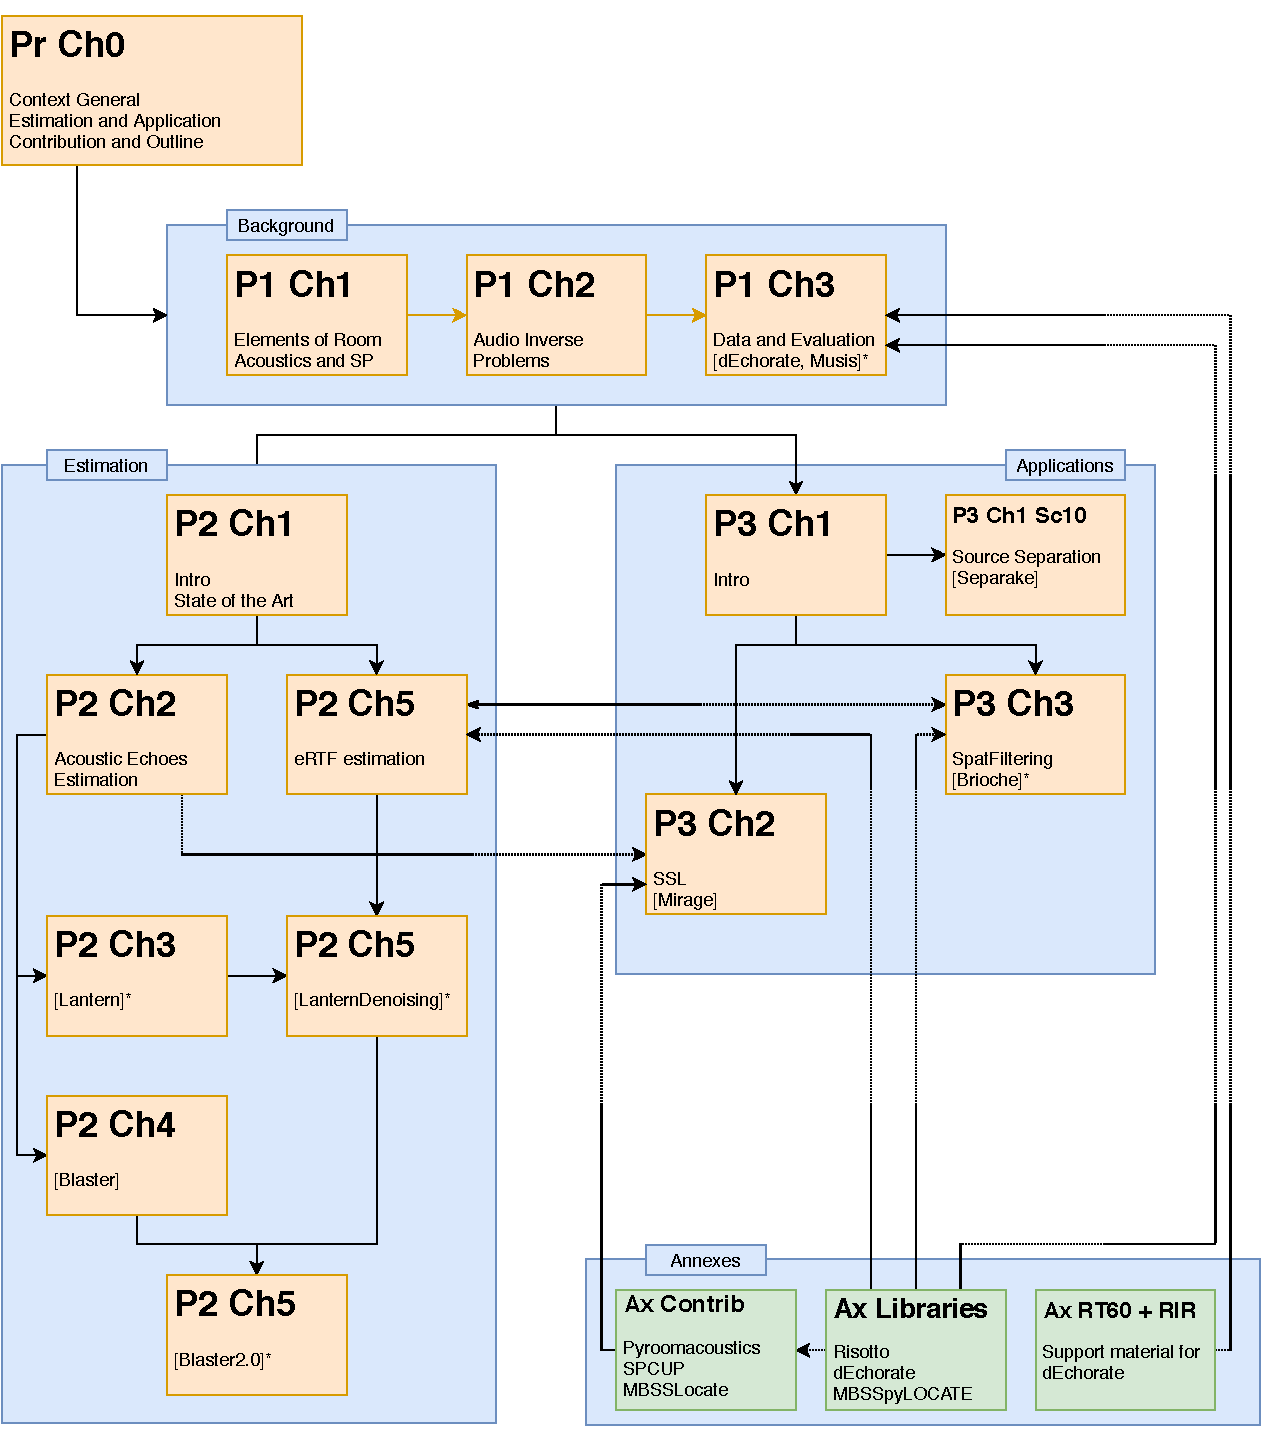
\includegraphics[width=\linewidth]{thesis_mindmap.pdf}
        \end{sidecaption}
\end{figure}

\section{Citation}
Using \detokenize{\citeonly{kuttruff2016room}} it will be like this \citeonly{kuttruff2016room}.
\\Otherwise using \detokenize{\cite{kuttruff2016room}} it will be like this \cite{kuttruff2016room}.
\\Otherwise using \detokenize{\citeauthor{kuttruff2016room}} it will be like this \citeauthor{kuttruff2016room}.


\section{Todos and Notes}

\itodo{Can we use \bison/'s argument (regarding differential cryptanalysis) for a maximal unbalanced Feistel network?}
\miss{Here something is missing}
\todo[inline]{The original todo note withouth changed colours.\newline Here's another line.}

\lipsum[11]\unsure{Is this correct?}\unsure{I'm unsure about also!}
\lipsum[11]\change{Change this!}
\lipsum[11]\info{This can help me in chapter seven!}
\lipsum[11]\plus{What was I thinking?!}
\lipsum[11]
\plus[inline]{The following section needs to be rewritten!}
\lipsum[11]

% \newthoughtpar{Incentives for new Cipher Designs}
% \blindtext

% \section{Section 1}
% \blindtext[3]

% \marginpar{%
%     \footnotesize
%     \vspace{\baselineskip}
%     \vspace*{-7\baselineskip}
%     See \cref{ch:intro} for a detailed explanation of differential cryptanalysis
%     and the problems that appear when trying to bound the differential probability.
% }

% \begin{problem}[Differentials]\label{prob:differentials}
%     \blindtext
% \end{problem}



% \section{Publications}

% During the course of my doctoral studies, I worked on several projects which are not all covered in the remainder of this thesis.
% In particular, these are the following.

% \newthoughtpar{Conference Publications}
% \begin{itemize}
% \item[] \fullfullcite{EC:CLLNW19}, see \cref{ch:bison}.
% %Because \bison/ can only be instantiated with odd block length, we here also give a second instance of the underlying construction: \wisent/.
% %This instance is for the even block length case and basically inherits almost the same security bounds as \bison/.
% \end{itemize}

% \newthoughtpar{Journal Publications}
% \begin{itemize}
%     \item[] \fullfullcite{ToSC:KraLeaWie17}.
%     \item[] \fullfullcite{ToSC:KLSW17}, see \cref{ch:slp}.
%     \item[] \fullfullcite{ToSC:LeaTezWie18}, see \cref{ch:st}.
% \end{itemize}


% \section{Stir of Echoes}

% \blindtext

% \section{Equations}

\begin{align}
    f(x) &= x^2\\
    g(x) &= \frac{1}{x}\\
    F(x) &= \int^a_b \frac{1}{3}x^3
\end{align}


A simple equation:
\[
 f(x)=(x+a)(x+b)
\]
An equation with text:
\begin{equation}
50 \text{ apples} \times 100 \text{ apples} =
\textbf{lots of apples}
\end{equation}
One including subscripts and superscripts:
\[ k_{n+1} = n^2 + k_n^2 - k_{n-1} \]
\section{Greek Letters}
\[ \alpha,  \beta,  \gamma, \Gamma, \pi, \Pi, \phi, \varphi, \mu, \Phi, \xi, \zeta \]
\[ \cos(2\theta\phi) = \cos^2 \theta\phi - \sin^2 \theta\phi \]
\section{Delimiters}
There are many types of delimiters one can use:
\[ ( a ), [ b ], \{ c \}, | d |, \| e \|,
\langle f \rangle, \lfloor g \rfloor,
\lceil h \rceil, \ulcorner i \urcorner \]
See how the delimiters are of reasonable size in these examples
\[
        \left(a+b\right)\left[1-\frac{b}{a+b}\right]=a\,,
\]
\[
        \sqrt{|xy|}\leq\left|\frac{x+y}{2}\right|,
\]
even when there is no matching delimiter
\[
        \int_a^bu\frac{d^2v}{dx^2}\,dx
        =\left.u\frac{dv}{dx}\right|_a^b
        -\int_a^b\frac{du}{dx}\frac{dv}{dx}\,dx.
\]
whereas vector problems often lead to statements such as
\[
        u=\frac{-y}{x^2+y^2}\,,\quad
        v=\frac{x}{x^2+y^2}\,,\quad\text{and}\quad
        w=0\,.
\]
\section{Multiple Fractions}
Typesetting continued fractions is easy:
\[
x = a_0 + \frac{1}{a_1 + \frac{1}{a_2 + \frac{1}{a_3 + a_4}}}
\]
However, as the fractions continue, they get smaller. If you want to keep the size consistent, use the display style; e.g.
\[
  x = a_0 + \frac{1}{\displaystyle a_1
          + \frac{1}{\displaystyle a_2
          + \frac{1}{\displaystyle a_3 + a_4}}}
\]
\section{Arrays}
Arrays of mathematics are typeset using one of the matrix environments as
in
\[
        \begin{bmatrix}
                1 & x & 0 \\
                0 & 1 & -1
        \end{bmatrix}\begin{bmatrix}
                1  \\
                y  \\
                1
        \end{bmatrix}
        =\begin{bmatrix}
                1+xy  \\
                y-1
        \end{bmatrix}.
\]
\[ \begin{pmatrix}
2 & 3 & 4\\
5 & 6 & 7\\
8 & 9 & 10 \end{pmatrix} v = 0 \]
Case statements use cases:
\[
        |x|=\begin{cases}
                x, & \text{if }x\geq 0\,,  \\
                -x, & \text{if }x< 0\,.
        \end{cases}
\]
Many arrays have lots of dots all over the place as in
\[
        \begin{matrix}
                -2 & 1 & 0 & 0 & \cdots & 0  \\
                1 & -2 & 1 & 0 & \cdots & 0  \\
                0 & 1 & -2 & 1 & \cdots & 0  \\
                0 & 0 & 1 & -2 & \ddots & \vdots \\
                \vdots & \vdots & \vdots & \ddots & \ddots & 1  \\
                0 & 0 & 0 & \cdots & 1 & -2
        \end{matrix}
\]
\section{Greek Letters}
\[ \alpha,  \beta,  \gamma, \Gamma, \pi, \Pi, \phi, \varphi, \mu, \Phi, \xi, \zeta \]
\[ \cos(2\theta\phi) = \cos^2 \theta\phi - \sin^2 \theta\phi \]
\section{Delimiters}
\[ ( a ), [ b ], \{ c \}, | d |, \| e \|,
\langle f \rangle, \lfloor g \rfloor,
\lceil h \rceil, \ulcorner i \urcorner \]
\section{Accents}
Mathematical accents are performed by a short command with one
argument, such as
\[
        \tilde f(\omega)=\frac{1}{2\pi}
        \int_{-\infty}^\infty f(x)e^{-i\omega x}\,dx\,,
\]
or
\[
        \dot{\vec \omega}=\vec r\times\vec I\,.
\]
\section{Multiline equations and aligned environments}
New lines (\\ ) do not work in equation environments. To achieve alignment of equations, use the aligned  package to produce multiline aligned math, such as:
\newline

% \[
% \begin{center}
% \begin{aligned}
% $F$ ={} & $\{F_{x} \in  F_{c} : (|S| > |C|)$ \\
%       & $\cap (\mathrm{minPixels}  < |S| < \mathrm{maxPixels})$ \\
%       & $\cap (|S_{\mathrm{conected}}| > |S| - \epsilon) $\}
% \end{aligned}
% \end{center}
% \]

% \newline

% and also:

% \newline
% \[
% \begin{center}
% \begin{aligned}
% $A_0$ & $=   \frac{1}{(\alpha+t_x)^{r+s+x}}{}_2 F_1\left( r+s+x,x+1;r+s+x+1;\frac{\alpha-\beta}{\alpha + t_x} \right) $\\
% & $\quad - \frac{1}{(\alpha+T)^{r+s+x}}{}_2 F_1\left( r+s+x,x+1;r+s+x+1;\frac{\alpha-\beta}{\alpha + T} \right),$
% \end{aligned}
% \end{center}
% \]
% \newline

\textbf{Note}: the above multiline equations have math mode defined per line, not globally at the equation level.
\section{Theorems and sets}

% \newtheorem{theorem}{Theorem}
% \newtheorem{corollary}[theorem]{Corollary}
% \newtheorem{lemma}[theorem]{Lemma}
% \newtheorem{definition}[theorem]{Definition}

\begin{theorem}
For any nonnegative integer $n$, we have
$$(1+x)^n = \sum_{i=0}^n {n \choose i} x^i$$
\end{theorem}
The Taylor series expansion for the function $e^x$ is given by
\begin{equation}
e^x = 1 + x + \frac{x^2}{2} + \frac{x^3}{6} + \cdots = \sum_{n\geq 0} \frac{x^n}{n!}
\end{equation}
\[ \forall x \in X, \quad \exists y \leq \epsilon \]
\[ \frac{n!}{k!(n-k)!} = \binom{n}{k} \]
\begin{theorem}
For any sets $A$, $B$ and $C$, we have
$$ (A\cup B)-(C-A) = A \cup (B-C)$$
\end{theorem}

\blindtext
\blinditemize

\blindtext
\blindenumerate

\blindtext
\blinddescription
    \chapter{Coding}

    \chapter{RIR and RT60 measurements}
\end{appendices}
% Diego Di Carlo
% diego.di-carlo@inria.fr

% === BIBLIOGRAPHY ===

\clearpage
% \phantomsection
% \addcontentsline{toc}{chapter}{Bibliography}
\begin{fullwidth}
    \printbibliography{}
\end{fullwidth}

\cleardoublepage{}

% % Diego Di Carlo
% diego.di-carlo@inria.fr

% === INDEX ===

\printindex
\addcontentsline{toc}{chapter}{Index}



\end{document}
